% !TEX program=luatex

\documentclass[12pt]{report}
\usepackage[Glenn]{fncychap}
\usepackage[T1]{fontenc}
\usepackage[francais]{babel}
\usepackage{fontspec}
\usepackage{wrapfig}
\usepackage{graphicx}
\usepackage{soul}
\usepackage[colorlinks=true, linkcolor=black, urlcolor=black, citecolor=black]{hyperref}
% \usepackage[hyphens, spaces, obeyspaces]{url}
\usepackage[a4paper, width=150mm, top=25mm, bottom=25mm]{geometry}
\usepackage{parskip}
\usepackage{enumitem}
\usepackage{titlesec}
\usepackage{listings}
\usepackage{float}
\usepackage[final]{pdfpages}
\usepackage{xcolor}
\usepackage{tocbibind}
\usepackage{tocloft}
\usepackage{xpatch}
\usepackage{amsmath}
\usepackage{amsthm}
\usepackage{amsfonts}
\usepackage{graphics}
\usepackage{color}
% \usepackage[grey,utopia]{quotchap}
\usepackage{moreverb}
\usepackage{xcolor}
\usepackage{framed}
\usepackage{arabluatex}
\usepackage[algo2e, french, onelanguage, ruled]{algorithm2e}
\setlist[itemize]{label=\textbullet}
\usepackage{fancyhdr}
\pagestyle{fancy}   
\fancyhead{}
\fancyhead[C]{\leftmark}
\renewcommand{\headrulewidth}{0.4pt}
\renewcommand{\footrulewidth}{0.4pt}
\usepackage{xcolor}
\definecolor{light-gray}{gray}{0.90}
\newcommand{\code}[1]{\colorbox{light-gray}{\texttt{#1}}}
\usepackage{listings}
\usepackage{multirow}

\usepackage{array}
\newcolumntype{L}[1]{>{\raggedright\let\newline\\\arraybackslash\hspace{0pt}}m{#1}}
\newcolumntype{C}[1]{>{\centering\let\newline\\\arraybackslash\hspace{0pt}}m{#1}}
\newcolumntype{R}[1]{>{\raggedleft\let\newline\\\arraybackslash\hspace{0pt}}m{#1}}

\lstdefinestyle{code}{
language=python,                   
keywordstyle=\color{blue},      
stringstyle=\color{blue},        
commentstyle=\color{gray},     
basicstyle=\small\ttfamily,           
numbers=left,                   
numberstyle=\normalsize,        
numbersep=7pt,                  
showstringspaces=false,         
breaklines=true,                
frame=leftline,                 
framerule=2pt,
}

\lstdefinestyle{api}{
language=python,                   
keywordstyle=\color{blue},      
stringstyle=\color{blue},        
commentstyle=\color{gray},     
basicstyle=\small\ttfamily,           
% numbers=false,                   
numberstyle=\normalsize,        
numbersep=7pt,                  
showstringspaces=false,         
breaklines=true,                
frame=leftline,                 
framerule=2pt,
}



%~~~BEGIN~~~%
\begin{document}
\pagenumbering{gobble}
\renewcommand{\contentsname}{Sommaire}
\tableofcontents
\clearpage

\listoffigures
\clearpage

\listoftables
\clearpage

\listofalgorithmes
\clearpage

\pagenumbering{roman} 
\newpage
\newpage
\vspace*{1.2cm}
\begin{center}
    \Large
    \textbf{Déclaration de non-plagiat}
\end{center}
\vspace*{2.5cm}
Nous, soussignés :
\vspace*{0.5cm}

M. Mohamed Fawzi TOUATI et\\
M. Saïd ZIANI,
\vspace*{1cm}

auteurs de ce mémoire de fin d'études de master N\textsuperscript{o} 069/2018, intitulé :
\begin{center}
\large
\textbf{
Réalisation d'un outil de revue de presse personnalisé
}
\end{center}
\vspace*{1.2cm}


déclarons, chacun, sur l'honneur que le présent mémoire est un travail original, et que n'avons ni recopié ni utilisé des idées ou des formulations tirées d'un ouvrage, article ou mémoire, en version imprimée ou électronique, sans mentionner précisément leur origine et que les citations intégrales sont mentionnées selon les règles scientifiques connues. 

Nous comprenons que le plagiat est un acte de malhonnêteté intellectuelle contraire à l'éthique académique et peut inclure des mesures disciplinaires tel que stipulé dans le règlement intérieur de l'USTHB.


\vspace*{3cm}
\textbf{Signatures :}



\vspace*{4cm}
\hspace*{8.5cm}
\textbf{Alger, Mardi 05 Juin 2018.}


\chapter*{Remerciements}    
%!TEX program=luatex

\vspace{1.5cm}

\setlength{\parindent}{0.5cm}
Avant tout, je remercie ALLAH le tout-puissant de m'avoir donné le courage, la volonté et la patience de mener à terme ce présent travail dans les meilleures conditions.

Je tiens à exprimer toute ma reconnaissance à mon encadreur principal, Monsieur Ahmed Guessoum. Je le remercie de m’avoir encadré, orienté, aidé et conseillé, et pour la liberté de travail qu'il m'a laissée tout au long de ce semestre. 
Je le remercie aussi pour sa disponibilité, sa patience et surtout ses judicieux conseils, qui ont contribué à alimenter ma réflexion.

J’adresse mes remerciements à mon Co-Encadreur, Monsieur Riadh Belkebir, pour ses paroles, conseils et critiques.

J'adresse également, mes remerciements à Madame Khellaf qui nous fait l'honneur de présider le jury de notre soutenance. Mes remerciements s’adressent également à Madame Abdat pour avoir accepté de faire partie de ce jury.

J’adresse mes sincères remerciements à tous les professeurs de l'USTHB , intervenants, et toutes les personnes qui par leurs paroles, leurs écrits, leurs conseils et leurs critiques ont guidé mes réflexions et ont accepté de me rencontrer et répondre à mes questions durant mon cursus et mes recherches et qui doivent voir dans ce travail la fierté d'un savoir bien acquis.

Je remercie mes très chers parents, qui ont toujours été là pour moi. Ma mère, qui a œuvré pour ma réussite, de par son amour, son soutien, tous les sacrifices consentis et ses précieux conseils, pour toute son assistance et sa présence dans ma vie : reçois à travers ce travail aussi modeste soit-il, l'expression de mes sentiments et de mon éternelle gratitude. Mon père, qui peut être fier et trouver ici le résultat de longues années de sacrifices et de privations pour m'aider à avancer dans la vie. Puisse Dieu faire en sorte que ce travail porte son fruit ; merci pour les valeurs nobles, l'éducation et le soutien permanent venu de toi.

« Vous avez tout sacrifié pour vos enfants n’épargnant ni santé ni efforts. Vous m’avez donné un magnifique modèle de labeur et de persévérance. Je suis redevable d’une éducation dont je suis fier ».
Je remercie mon frère et ma sœur pour leur encouragement. Ma pensée va également à mon grand père, et toute ma famille qui m'ont encouragé pendant ce travail.

Je tiens à  remercier en particulier Nadjib et Billel pour leur appui lors de mes stages en externe durant tout mon cursus.
J'adresse tous mes voeux de réussite à Saïd ziani (mon binôme), ainsi que tous les autres étudiants en Master 2 SII spécialement et les autres Masters en général.

Enfin, je remercie tous mes Amis que j’aime tant, Karim, Nidal, Salim, Haithem, Houssem, Driss, Nabil, Said, Lahcen, Anis, Walid, Hichem, et tous mes autres ami(e)s pour leur sincère amitié et confiance, et à qui je dois ma reconnaissance et mon attachement.

À tous ces intervenants, je présente mes remerciements, mon respect et ma gratitude.

\vspace{0.5cm}
\begin{center}
\Large
\hspace{12.5cm}
\textbf{Fawzi}
\end{center}
\chapter*{Remerciements}    
%!TEX program=luatex

\begin{center}
    \Large
    \textbf{Saïd}
\end{center}

\vspace{1cm}

\setlength{\parindent}{0.5cm}
Avant toute chose, j'adresse mes remerciements au bon Dieu pour m'avoir donné la force et le courage de mener à terme ce modeste travail.

Toute ma reconnaissance, mon admiration et ma profonde gratitude vont vers notre promoteur, le Professeur Ahmed GUESSOUM, d'abord pour le sérieux, le niveau et la qualité de ses enseignements mais aussi pour son accompagnement, ses conseils précieux et sa patience tout le long de notre projet de fin d'études de master. Merci monsieur.

Je remercie également mesdames les membres du jury, Mme. F. KHELLAF et Mme. N. ABDAT d'avoir accepté d'examiner et de juger notre travail.

Je n'oublie pas de remercier mon binôme Fawzi pour son sérieux et sa patience.

Que tous ceux qui, de près ou de loin, ont contribué par leurs conseils, leurs encouragements ou leur amitié à l'aboutissement de ce travail, trouvent ici l'expression de ma profonde reconnaissance.

Pour leur soutien moral et la patience qu'ils m'ont manifestée durant tout le cursus universitaire et scolaire, je remercie fortement tous les membres de ma famille.

Enfin, remercier mes parents serait se répéter, parfois pour exprimer plus que ce qu'on a envie de dire on a recours au silence.


\chapter*{Dédicaces}    
\begin{center}
    \Large
    \textbf{Fawzi}
\end{center}

\vspace{1cm}

Je dédie ce modeste travail à :

Mes parents. Aucun hommage ne pourrait être à la hauteur de l’amour dont ils ne cessent de me combler. Que dieu leur procure bonne santé et longue vie.

Toute ma famille, et mes amis, A mon binôme Saïd et à tous ceux qui ont contribué de près ou de loin pour que ce projet soit possible, je vous dis merci.
\chapter*{Dédicaces}    


\vspace{1.5cm}


Ce modeste travail est dédié,

À mes chers parents, à qui aucun hommage ne pourrait être à la hauteur de leurs sacrifices. Que Dieu leur procure bonheur et longue vie.

À mes frères et sœurs Lies, Wissem, Amira et Rima que j'aime énormément.

À tous mes amis en particulier Sabrina, Yanis, Sidahmed, Arslan, Mourad, Kamel et à tous les Apôtres pour leur présence et leur soutien.
% À tous mes amis en particulier Sabrina, Yanis, Sidahmed, Arslan, Mourad et Kamel pour leur présence et leur soutien.

À tous les membres d'OpenMindsClub et la communauté du Libre/Open source, ma deuxième famille. 

Et à toute personne qui, de près ou loin, m'a apporté soutien, conseil ou réconfort. 

Mille mercis.\\

\vspace{0.5cm}
\begin{center}
\Large
\hspace{12.5cm}
\textbf{Saïd}
\end{center}


\newpage
%!TEX program=luatex
\begin{center}
    \Large 
    \textbf{Résumé}
\end{center}

Avec l'émergence des TIC et la démocratisation de la production de contenu sur internet, on assiste à un tsunami informationnel. Ce dernier est très difficile à gérer manuellement, et même les outils informatiques classiques peinent à offrir des résultats concluants. Les journaux et les sites d'information contribuent pleinement à ce contenu, ce qui rend la revue de presse quotidienne dure à appréhender. 

Notre projet, propose un outil sophistiqué qui prend en considération les centres d’intérêt de chaque utilisateur, afin de lui suggérer les articles les plus pertinents de la presse algérienne et internationale, et ce dans les deux langues (Arabe et Anglais). Ceci est accompli en utilisant des techniques d'intelligence artificielle, de traitement automatique du langage et d'apprentissage automatique. 

\noindent
\textbf{Mots clés :} Traitement automatique du langage naturel, catégorisation de textes, corpus de résumé
automatique, résumé automatique, traduction automatique, profilage d'utilisateurs, recommandation d'articles de presse.  

\vspace*{0.8cm}

\begin{center}
    \Large 
    \begin{arab}
    ملخص
    \end{arab}
\end{center}
\begin{arab}
مع بروز تكنولوجيا الإعلام و الإتصال و دمقرطة محتوى صفحات الأنترنت، أصبح التحكم في الكم الهائل من المعلومات صعبا للغاية، سواءا يدويا أو حتى باستعمال أنظمة معلوماتية. وتساهم الصحف و المواقع الإخبارية بشكل مباشر في تزايد المحتوى، مما يجعل الإطلاع على الأخبار أمرا متعبا يتطلب الكثير من الوقت. 

لمعالجة هذه الإشكالية، نقترح في مشروعنا تطبيقا يأخذ بعين الإعتبار اههتمامات المستخدمين بهدف اقتراح مقالات من الصحافة الجزائرية و الدولية باللغتين العربية و الإنجليزية تلبي رغبة القارئ، و هذا باستخدام تقنيات الذكاء الإصطناعي و المعالجة الآلية للنصوص.

\textbf{الكلمات الدالة :} المعالجة الآلية للغات،  تصنيف النصوص، تلخيص النصوص، الترجمة الآلية، التوصية.  
\end{arab}

\vspace*{0.8cm}


\begin{center}
    \Large 
    \textbf{Abstract}
\end{center}

With the internet playing such an important part in our lives, especially in the way we communicate through it (social media, blogs, etc), it has become very difficult to control the flow of information, whether manually or even by using IT solutions.

Reading magazines and newspapers has become very time consuming, considering the huge amount of online content and the speed with which this content is updated.

Our solution considers each user's centers of interest in order to suggest to him/her articles from the internet, articles that are relevant to each one of them. For this purpose we use Artificial Intelligence, Machine Learning and Natural Language Processing.

\noindent
\textbf{Keywords :} Natural Language Processing, Text classification, Automatic summarization corpora, automatic summarization, Machine translation, user profiling, news recommendation. 

\newpage
\pagenumbering{arabic} 
\chapter*{Introduction générale}    
%!TEX program=luatex

Voilà maintenant vingt ans que les premiers journaux occidentaux (américains et européens) ont commencé la diffusion de l'information sur le web. Les premiers sites web des quotidiens d'information sont apparus en 1995. Rapidement, toutes les organisations de presse se sont tournées vers le média en ligne, Internet.

Dès les années 90, de nombreux sites diffusent des informations d'actualité alors qu'ils n'ont rien à voir avec le journalisme. Dans la même décennie, plusieurs formes de sites d'informations sont nées, entre blogs, webzines (magazines en ligne) ou sites indépendants. De nos jours, et avec l'émergence des Technologies de l'Information et de la Communication et la démocratisation de la production de contenu sur internet, le nombre de sites d'informations et les quantités énormes de contenu créé ne cessent d'augmenter exponentiellement chaque jour.

En Algérie, comme partout dans le monde, les acteurs médiatiques, notamment des journaux et des chaînes télévisées, ont vu leurs canaux de communication muer et leur digitalisation se développer progressivement au point où certains utilisent le web comme unique médium. On peut citer TSA (Tout Sur l'Algérie), Algérie Focus, Casbah Tribune, etc.

Avec toutes ces quantités informationnelles et ce nombre croissant de médias en ligne, le lecteur algérien, ou autre, se trouve incapable de traiter ce flux d'informations manuellement, et même les outils technologiques (classiques) ne remédient pas à cette problématique. C'est la raison principale pour laquelle il a été jugé utile de concevoir et de réaliser un outil qui permet à l'utilisateur d'exploiter, de la façon la plus efficace possible, toutes ces ressources en se basant sur ses préférences.

L'outil que nous proposons utilisera des techniques d'intelligence artificielle, de traitement automatique du langage, d'apprentissage automatique, de recherche d'information et de recommandation personnalisée. En se basant sur ces derniers, notre solution sera capable d'aider le lecteur à faire sa revue de presse quotidienne de la manière la plus enrichissante possible, mais aussi la plus optimale. Et en utilisant des techniques de profilage intelligent, les recommandations d'articles de presse seront adaptées aux centres d'intérêts et préférences de chaque utilisateur, et seront plus précises avec le temps grâce aux évaluations des suggestions précédentes.

Et dans l'optique de rendre cet outil plus sophistiqué, nous proposons à l'utilisateur un accès efficace à un contenu anglophone avec possibilité de traduction automatique. Nous mettrons en place également une fonctionnalité de génération de résumé automatique pour chaque article, ce qui sera d'une grande aide à toute personne voulant gagner du temps, notamment les professionnels du domaine journalistique, politique ou des affaires, devant faire la veille de toutes les dernières actualités.

Pour ce faire, nous étudierons les concepts théoriques de base de chaque technique tout en examinant la littérature et les travaux de l'état de l'art. Nous allons, ensuite, travailler sur la conception des différents modules du système. Et enfin, nous passerons à la réalisation qui sera suivie par tests et évaluations.

Le premier chapitre de ce mémoire consistera en la présentation des systèmes de recommandations. Le deuxième portera sur le traitement Automatique du Langage Naturel. Le troisième, quant à lui, fera l'objet de l'étude conceptuelle. Enfin, dans le quatrième et dernier chapitre, nous présenterons le produit final ainsi que sa réalisation. Puis, avant de parler des perspectives possibles et de l'avenir de notre application, nous dresserons une conclusion générale du projet.

% Le présent travail est ainsi divisé en quatre chapitres. 
% \begin{itemize}[leftmargin=*,label={-}]
%     \item Le chapitre 1 s'intitule Les systèmes de recommandations.
%     \item Le chapitre 2 porte sur le traitement Automatique du Langage Naturel.
%     \item Le chapitre 3, quant à lui, décrit notre conception.
%     \item Et enfin, le chapitre 4 présente la réalisation.
% \end{itemize}

\chapter{Systèmes de recommandations}
%!TEX program=luatex

\newpage
\section{Introduction}
Les systèmes de recommandation demeurent aujourd'hui un moyen non négligeable pour l'amélioration de l’expérience utilisateur sur les réseaux sociaux, le e-commerce et sur les moteurs de recherche.\\
Ils contribuent d'une manière considérable dans l'accroissement de plusieurs entreprises technologiques tels que \emph{Facebook}, \emph{Amazon} ou \emph{Google} qui exploitent des quantités massives de données (Big data) afin de faire des recommandations avec un niveau de confiance assez élevé.\\
Il sera question dans ce chapitre d’effectuer une description de l'état de l'art par la présentation des systèmes de recommandations et leurs utilisations pour la prédiction des comportements des utilisateurs, une brève présentation de l'apprentissage automatique et ses différentes techniques, et nous allons conclure par l'introduction des techniques de profilage d'utilisateurs.

\section{Apprentissage automatique}
    \subsection{Définition}
    \emph{L'apprentissage automatique} comme il a été défini par \emph{svensson} et \emph{Söderberg} dans leur article «Machines that learn»\cite{svensson} désigne la conception et le développement d'algorithmes et de techniques qui permettent aux ordinateurs d'apprendre et de prédire de façon intelligente.\\
    Souvent on a recours à l'apprentissage automatique lorsque on ignore le modèle adéquat à utiliser pour la résolution d'un problème donné, on peut citer aussi :
    \begin{itemize}
        \item Le manque d'expertise sur le problème.
        \item La difficulté et la complexité des solutions disponibles. 
        \item L'espace des solutions du problème est très grand et change dans le temps. 
    \end{itemize}
    L'apprentissage automatique est utilisé dans différents domaines: économie, divertissement et multimédia.

    \subsection{Le processus d'apprentissage}
    Afin d'implémenter un modèle performant et précis, certains pré-traitements doivent être fait comme le précise Han dans son livre «DATA MINING Concepts»\cite{Han}, on retrouve:

    \begin{itemize}
    	\item Collecte des données : le but de cette étape est de récupérer les données représentatives et qui ont un sens par rapport au problème traité.
    	\item Séléction des caractéristiques (Features) : c'est l'étape la plus importante de ce processus, la performance du modèle finale y dépend.
    	\item Nettoyage de données : suppression des données aberrantes et remplacement des valeurs manquantes, normalisation et discrétisation.
    	\item Choix du type d'apprentissage selon le problème posé.
    	\item Apprentissage.
    	\item Évaluation : Évaluer les capacités prédictives du modèle et sa généralisation, et comparer ces performances par rapport a d'autres techniques.
    \end{itemize}

    \subsection{Paradigmes de l'apprentissage automatique}
    Nous avons évoqué précédemment le type d'apprentissage a choisir dans le processus d'apprentissage, on peut trouver plusieurs algorithmes d'apprentissage automatique.\\
    Ces algorithmes peuvent être classés dans deux groupes basés sur la façon avec laquelle ils \emph{apprennent} à prédire : supervisé, non supervisé et par renforcement.

        \subsubsection{Apprentissage automatique supervisé}
        L'apprentissage supervisé est ainsi nommé car il nécessite l'intervention de l'être humain (souvent un expert) pour spécifier à l'algorithme les résultats qu'il devrait fournir.\\
        L'apprentissage supervisé nécessite que les sorties possibles de l'algorithme soient déjà connues et que les données utilisées pour former l'algorithme soient déjà étiquetées avec des réponses correctes. Donc, les données d'apprentissage doivent être labellisées/classifiées au préalable en plus des caractéristique d'identification.\\

        parmi les approches utilisées pour l'apprentissage automatique supervisé, on retrouve :

        \textbf{•La régression :} la régression est le problème de l'estimation ou de la prédiction d'une quantité continue. Combien de clients partiront pour un concurrent cette année? 
        ces algorithmes sont :L'analyse de régression fait partie de l'analyse prédictive et exploite la co-relation entre dépendante (cible) et variables indépendantes.\\
        Les modèles de régression notables sont: régression linéaire, régression logistique, pas à pas
        Régression, régression des moindres carrés ordinaires (OLSR), splines de régression adaptative multivariée (MARS), localement Lissage de nuage de points estimé (LOESS).\cite{surveymachinelearningregression}

        \textbf{•Classification:}
        La classification consiste à attribuer des observations à des catégories discrètes plutôt qu'à estimer des quantités continues exemple : Un client donné nous quittera-t-il pour un concurrent? Est-ce qu'un patient donné à un cancer?\\
        Les algorithmes pour effectuer la classification sont :

        - Algorithmes d'arbre de décision: Un arbre de décision construit une structure de type arbre de solutions possibles à un problème basé sur certaines contraintes.\\ 
        Il est ainsi nommé car il commence par une simple décision simple ou racine, qui se décompose ensuite en un certain nombre de branches jusqu'à ce qu'une décision ou une prédiction soit faite, formant un arbre.\\
        Ils sont favorisés pour sa capacité à formaliser le problème dans le processus de la main qui à son tour aide à identifier le potentiel solutions plus rapides et plus précises que d'autres. Exemples: Arbre de classification et de régression (CART), itératif Dichotomiseur 3 (ID3), C4.5 et C5.0, détection automatique d'interférence au chi carré (CHAID), souche de décision, M5, Arbres décisionnels conditionnels, etc.\cite{surveymachinelearningclassification}

        - Algorithmes bayésiens: Un groupe d'algorithmes ML utilise le théorème de Bayes pour résoudre les problèmes de classification et de régression.\\
        Exemples: Bayes naïves, bayes naïves gaussiennes, bayes naïves multinomiales, estimateurs à une dépendance en moyenne (AODE), Bayesian Belief Network (BBN), réseau bayésien (BN) etc.\cite{surveymachinelearningclassification}

        - Machine de vecteur de soutien (SVM): SVM est une technique ML si populaire qu'elle peut être un groupe à part entière. Utilise un hyperplan séparateur ou une décision Les limites de décision de plan todemarcate parmi un ensemble de points de données sont classées avec des étiquettes différentes.\\ 
        C'est strictement algorithme de classification supervisé. En d'autres termes, l'algorithme développe un hyperplan optimal en utilisant des données d'entrée ou données de formation et ce plan de décision à tour de rôle de nouveaux exemples.\\ 
        Basé sur le noyau utilisé, SVM peut effectuer classification linéaire et non linéaire.\cite{surveymachinelearningclassification}


        \subsubsection{Apprentissage automatique non-supervisé}
        L'apprentissage automatique non supervisé consiste à déduire une fonction à partir de données \textbf{non labellisées/étiquetées} en utilisant des algorithmes basés sur le calcul de la similarité entre ces données.\\
        Les données seront divisé en sous-groupes de manière que ces derniers seront le plus possible similaires.
        Ce type d'apprentissage est très utilisé dans le domaine de l'imagerie médical et la détection d'anomalie.\\
        La technique la plus utilisée est \textbf{le clustering}, la mise en cluster concerne l'utilisation d'un modèle intégré dans les ensembles de données pour classer et étiqueter les données en conséquence.\\
        Exemples: K-Means, K-Medians, Propagation d'Affinité, Clustering Spectral, Cluster hiérarchique Ward, Clustering agglomératif. DBSCAN, mélanges gaussiens, bouleau, décalage moyen, maximisation des attentes (EM), ...etc.\cite{surveymachinelearningclustering}

        \subsubsection{Apprentissage automatique par renforcement}
        Un type plus récent de problème d'apprentissage qui a acquis beaucoup de traction récemment s'appelle l'apprentissage par renforcement.\\ 
        Dans ce type d'apprentissage, aucun exemple n'est fourni a la machine sauf une information sous la forme d'un signal de récompense.\\ 
        Les méthodes d'apprentissage par renforcement ressemblent à la façon dont les humains apprennent: la machine essaie un tas de choses différentes et est récompensée quand elle fait quelque chose de bien.\\
        L'apprentissage par renforcement est utile dans les cas où l'espace de solution est énorme ou infini et s'applique généralement dans les cas où la machine peut être considérée comme un agent interagissant avec son environnement (Agent cognitif).


\section{Les systèmes de recommandations}
Un nombre croissant d'entreprises en ligne utilisent des systèmes de recommandation pour accroître l'interaction de l'utilisateur et enrichir le potentiel d'achat. Les cas d'utilisation des systèmes de recommandation ont connu une expansion rapide dans de nombreux aspects du commerce électronique et des médias en ligne au cours des cinq dernières années, et nous prévoyons que cette tendance se poursuivra.\\ 
Les systèmes de recommandation (souvent appelés «moteurs de recommandation») peuvent modifier la façon dont les sites Web communiquent avec les utilisateurs et permettre aux entreprises de maximiser leur retour sur investissement en fonction des informations qu'ils peuvent recueillir sur les préférences et les achats de chaque client.
    \subsection{Définition}
    Un système de recommandation est un mécanisme de filtrage de l'information qui permet de proposer à des utilisateurs des éléments qui sont susceptibles de les intéresser selon leurs préférences et leurs comportements.\\
    Le but final est de prédire leur appréciation afin de leur suggérer des éléments similaires qu'ils seraient en mesure d'apprécier.\\
    Ces systèmes utilisent des techniques très avancés de l'intelligence artificielle tels que l'apprentissage automatique, le traitement automatique de la langue et la recherche d'informations. 

    \subsection{Quelques exemples des systèmes de recommandations}
    Compte tenu de l'importance des systèmes de recommandation qui permettent de cibler l'utilisateur selon ses caractéristiques (profil), plusieurs modèle de ces derniers ont vue le jour. Nous allons expliciter quelques uns :

        \subsubsection*{Système de recommandation pour les réseaux sociaux :}
        \textbf{LinkedIn :} LinkedIn est un réseau social professionnel qui fait usage des systèmes de recommandation.Il utilise un filtrage collaboratif à base d'objets (Membres, Sociétés, Groupes) grâce à un module de recommandation disponible dans chaque profil permettant de recommander d'autres membres fréquemment associés au profil actuel ou du même groupe ou postulant au même emploi.\\
            \begin{figure}[H]
                \centering
                   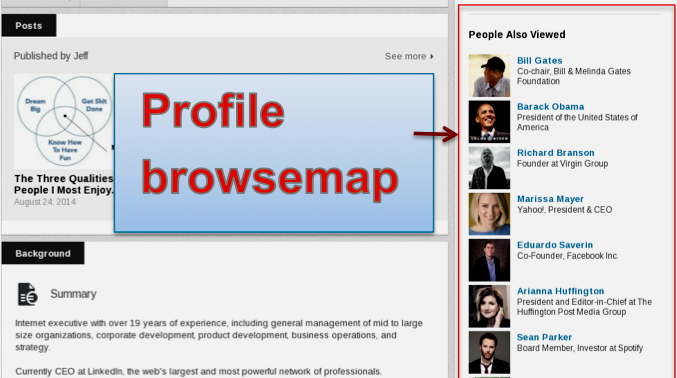
\includegraphics[height=180pt,width=350pt]{img/chapter1/linkedin.png}
                \caption{Recommandations sur le réseau social LinkedIn.}
            \end{figure}

        \textbf{Facebook :} Facebook est un réseau social en ligne qui permet aux 829 millions d’utilisateurs quotidien \cite{userFacebook} d'interagir avec d'autres personnes (et marques) autour du monde en partageant et en taggant des photos, en publiant des liens, en créant des groupes et des événements, en commentant et en chattant. Afin de recommander des amis, des groupes, des pages ou bien des événements, Facebook utilise plusieurs types de systèmes de recommandation tel que le filtrage collaboratif et le filtrage basé contenu.\\ 

        \subsubsection*{Système de recommandation pour les Plateformes de e-commerce :}
        \textbf{Amazon :} Amazon est un site internet de vente en ligne, très répandu dans le monde. Il compte selon \cite{refamazonus} 300 millions de comptes utilisateurs. Pour cela, le développement d'un système de recommandation était une tache majeure. Les ingénieurs d'Amazon ont opté depuis le début pour une approche basée sur un \emph{filtrage collaboratif basé mémoire} (memory-based collaborative filtering) qui permet de recommander les produits en se basant sur les produits préférés par les utilisateurs similaires mais aussi de cibler les produits similaires à ceux déjà achetés ou notés\cite{amazon}. Cette approche a été essentielle a Amazon puisque’elle représente à elle seule 35\% du chiffre d'affaires d'Amazon selon une étude de McKinsey's Chicago office \cite{McKinsey}.\\ 
            \begin{figure}[H]
                \centering
                   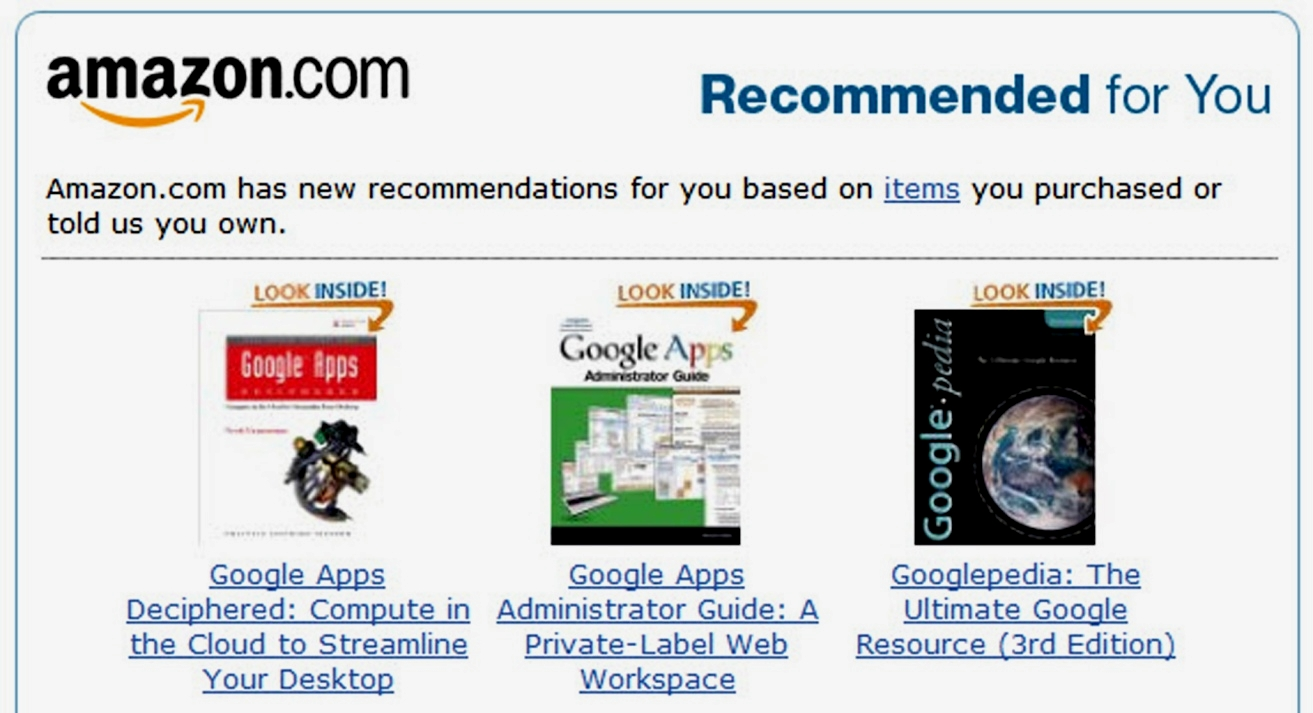
\includegraphics[height=180pt,width=350pt]{img/chapter1/amazon.jpg}
                \caption{Recommandations sur le site \emph{amazon.com}}
            \end{figure}

        \subsubsection*{Système de recommandation pour les plate-forme de streaming vidéo :}
        \textbf{Netflix :} Netflix est un média qui propose du contenu vidéo (films, séries, documentaires...) en flux continu sur internet. Comme ce site est très prisé partout dans le monde, Netflix se concentre beaucoup sur les systèmes de recommandation pour proposer les vidéos appropriées aux utilisateurs. Parmi les méthodes utilisées, on retrouve :
            \begin{enumerate}
                \item \textbf{Top-N VideoRanker :} C'est un algorithme permettant de retrouver les meilleures recommandations personnalisée pour chaque abonné en se basant sur le classement du nombre de vues des films, les tendances et la popularité.\\

                \item \textbf{Personnalized VideoRanker :} C'est un algorithme personnalisé qui se base sur le profil de l'utilisateur pour le classement de vidéo populaires. La précision amené par cet algorithme été nettement plus intéressante que l'algorithme précédent \cite{netflix} .\\

                \item \textbf{Tendances du moment :} Cet algorithme propose les tendances du moment combinés au profil utilisateur. Les tendances restent aussi un puissant moyen de prédiction.\\

                \item \textbf{Continuité :} C'est une solution qui propose un contenu vidéo qui est dans la continuité du contenu actuel comme le prochain épisode d'une série.\\

                \item \textbf{Filtrage par similarité entre vidéos :} C'est une solution permettant de prédire des vidéos de la même catégorie que la vidéo actuelle.\\

                \item \textbf{Génération des pages :} À la création du site, Netflix proposait de petites fenêtres sur les pages générées. Celles-ci représentaient les catégories et les genres des Films ou séries. À partir de 2015, les systèmes de recommandations ont rendu la génération des pages beaucoup plus personnalisés ce qui fait que certaines fenêtres inutiles ont disparu.\\

                \item \textbf{Évidence :} Cet algorithme recommande des films a l'utilisateur en utilisant certaines caractéristiques des films (acteurs fameux, oscars...).\cite{netflix}\\
            \end{enumerate}
            \begin{figure}[H]
                \centering
                   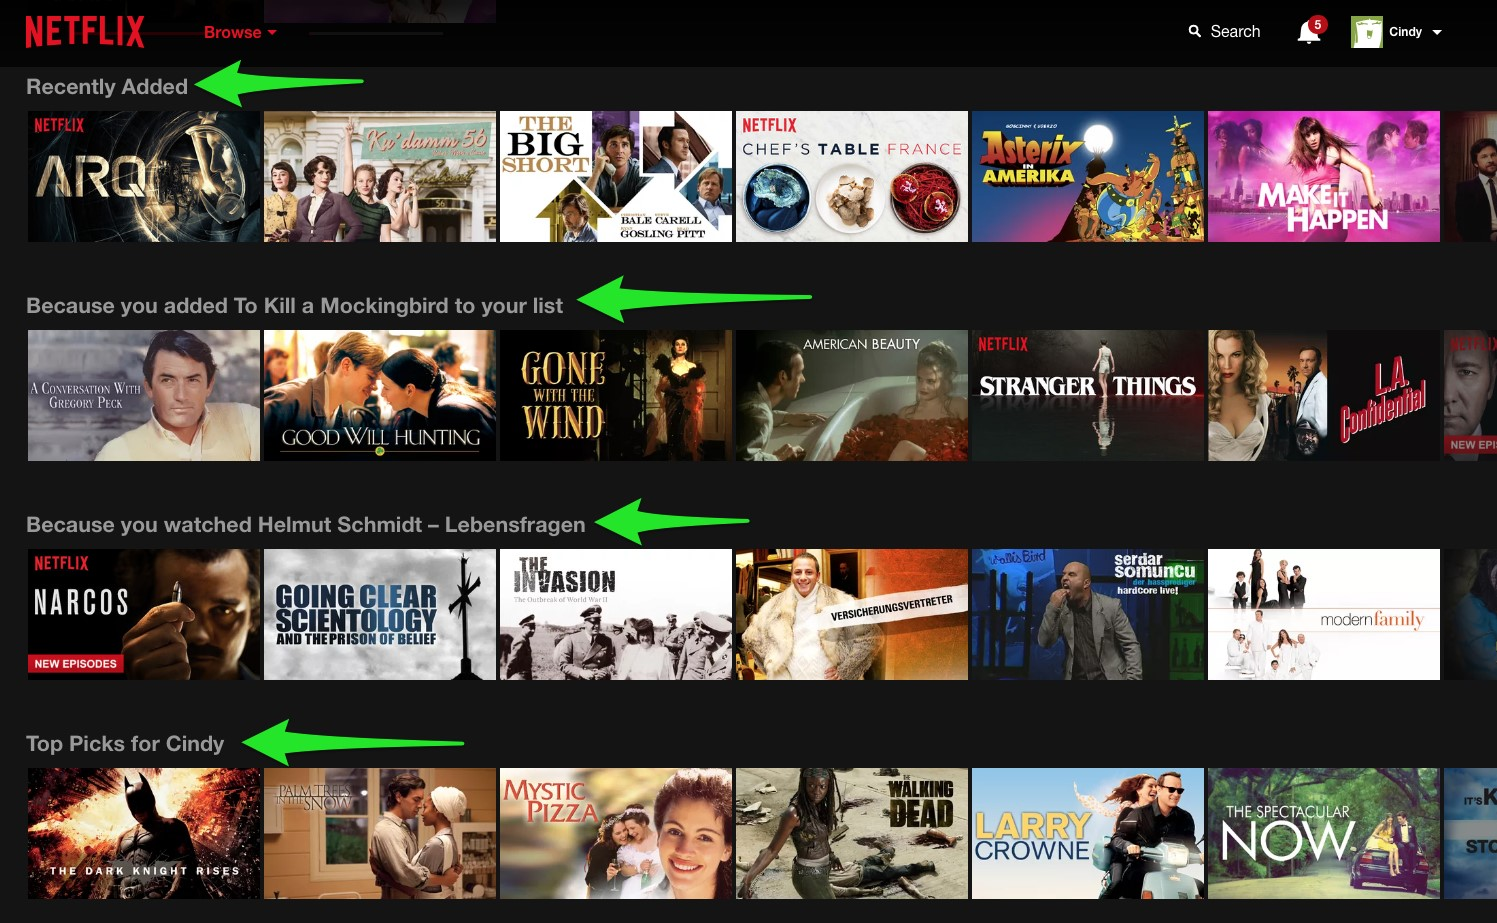
\includegraphics[height=180pt,width=350pt]{img/chapter1/netflix.jpg}
                \caption{Recommandations sur la plate-forme Netflix}
            \end{figure}

        \subsubsection*{Système de recommandation pour les articles de presse :} 
        \textbf{Google News :} c'est une plate-forme en ligne d'articles de presse obtenue de différentes sources. Initialement Google utilisait un filtrage collaboratif, ensuite ils ont combiné l'approche collaboratif et l'approche basée contenu pour offrir de meilleurs résultats.\cite{gglnews}

        \textbf{Buzzer :} c'est un système de recommandation développé par l'université de Dublin sur la base de nombre de clics limités sur des pages de presse en ligne. Ce laboratoire a testé des approches basées sur le public (\emph{rank}, \emph{friends rank} et \emph{content rank}). L'évaluation a permis de constater que le nombre de clics le plus important était généré par le \textbf{friends rank} a continuer .... c'est a dire friends rank.\cite{gglnews}\\
            \begin{figure}[H]
                \centering
                   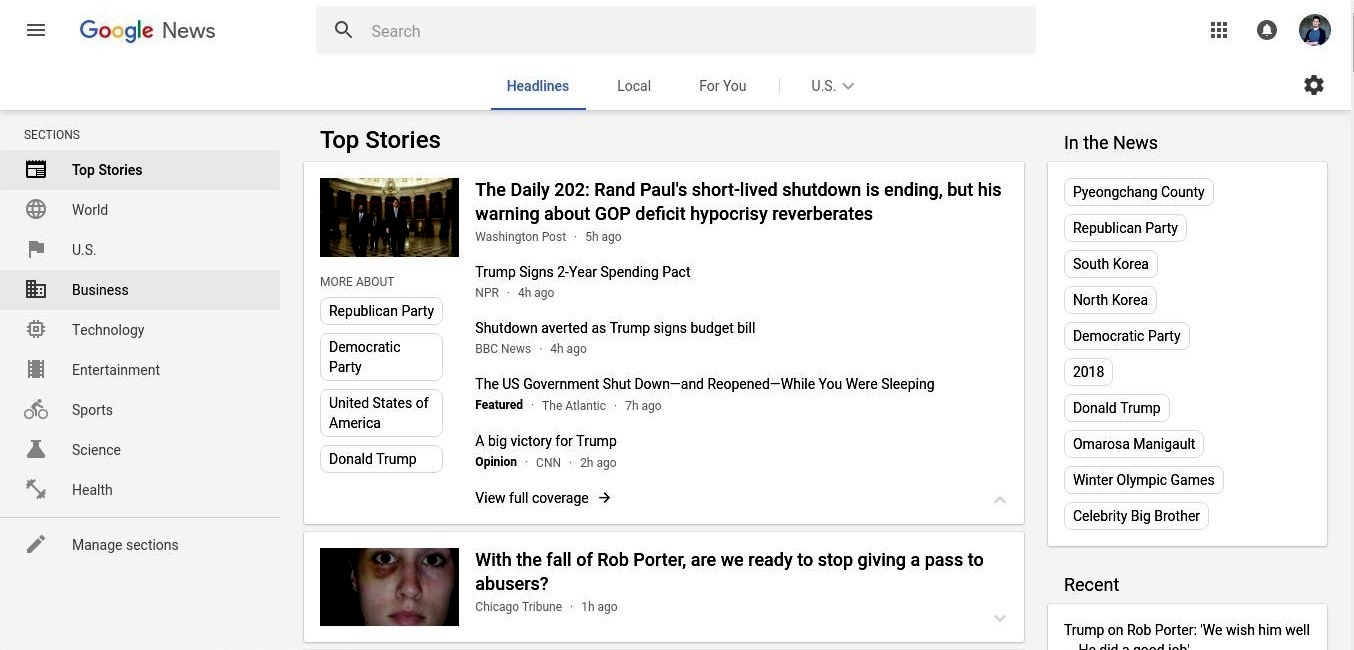
\includegraphics[height=180pt,width=350pt]{img/chapter1/news.jpg}
                \caption{Portail de GoogleNews avec des recommandations}
            \end{figure}

        Au terme de ce tour d'horizon, on constate que les systèmes de recommandations participent grandement à promouvoir les objets (produits, multimédia, articles de presse...) puisqu'ils représentent 80\% du contenu proposé. Ceci a diminué des activités des moteurs de recherche de chaque site décrit précédemment puisqu'elles représentent que 20\% des données proposées selon un article intitulé "The Netflix Recommender System:Algorithms,Business Value,and Innovation" apparu sur le site officiel de Netflix. \cite{netflix}\\

    \subsection{Types de systèmes de recommandations}
    définition en 1 ligne ou 2.
    \begin{figure}[H]
            \centering
               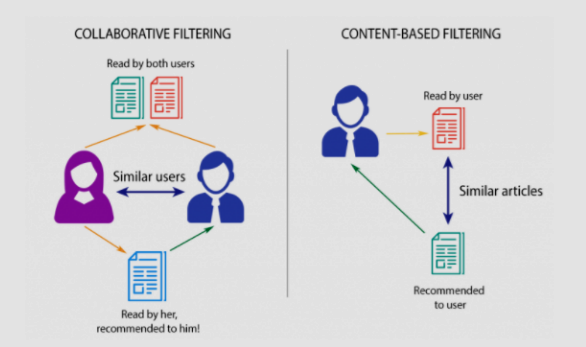
\includegraphics[height=180pt,width=350pt]{img/chapter1/filtering.png}
            \caption{Types de systèmes de recommandations\cite{figfiltering}}

    \end{figure}

    \begin{itemize}
        \item \textbf{Filtrage basé contenu (Content-based filtering) :\\}
        C'est une des méthodes de recommandation les plus simples; elle consiste à recommander les items ayant le plus de similarité avec les préférences de l'utilisateur.\\

        \item \textbf{Filtrage collaboratif (Collaborative filtering) :\\}
        Dans cette approche, la recommandation se fait en utilisant les préférences des profils jugés similaires au profil ciblé, et cela grâce aux préférences précédentes des personnes qui sont regrouper dans des structures de données permettant de calculer la similarité. Parmi les méthodes utilisées on retrouve :
            \begin{enumerate}
                \item \textbf{Filtrage collaboratif basé mémoire (Memory-based collaborative filtering) : }Les notes d'appréciation des utilisateurs sont utilisées pour le calcul de similarité entre utilisateurs ou entre les objets afin de permettre de cibler au mieux les préférences.\\
                \item \textbf{Filtrage collaboratif basé model (Model-based collaborative filtering) : }Cette technique utilise un modèle de prédiction propre à chaque utilisateur selon les techniques de DataMining, de Recherche d'Informations et de Traitement Automatique du Langage.\\
            \end{enumerate}

        \item \textbf{Filtrage hybride (Hybrid recommender system) :\\}
        Cette approche utilise filtrage basé contenu et le filtrage collaboratif pour faire face aux problèmes rencontrés en utilisant un filtrage basé contenu seul ou en utilisant un filtrage collaboratif seul. Le but est d'avoir une précision maximale c'est a dire de meilleurs capacités de prédiction.\cite{filtering}
    \end{itemize}

    \subsection*{Avantages des systèmes de recommandations}
    L'utilisation des systèmes de recommandations est une approche gagnante sur tout les fronts que ce soit pour un utilisateur qui trouve tout ce qu'il cherche de manière facile ou pour l'organisme qui désire générer des gains économiques rapidement et efficacement.\\
    En effet, les recommandations ciblent directement un article précis pour un utilisateur précis, ce qui va pousser ce dernier à s'accrocher et à continuer sa recherche afin de trouver la meilleure offre possible. D'un autre coté, l'utilisation des profils utilisateurs dans les systèmes de recommandations les rendent beaucoup plus personnalisés et conformes aux besoins réels de l'utilisateur.\cite{figfiltering}

\section{Systèmes de recommandations pour les articles de presse}
    \subsection*{Contraintes liées a la recommandation des articles de presse}
    L'utilisation des systèmes de recommandation pour des sites de vente en ligne ou des réseaux sociaux est très différente de son utilisation pour une revue de presse personnalisée, puisqu'ils y existent des contraintes spécifiques aux revues de presse.
    Parmi ces contraintes on retrouve :
    \begin{itemize}
        \item \textbf{Le démarrage à froid (Cold start) : \label{froid}}c'est à dire on ne possède aucune information précédente sur l'utilisateur, ses caractéristiques ou son profil. Généralement c'est lors d'une navigation sans identification que ce cas se présente.\\
        \item \textbf{Le manque de données (Data sparsity) : }les structures de données liées au profil de l'utilisateur peuvent être vides ou très denses ce qui nécessite pour les deux cas un traitement particulier.\\
        \item \textbf{La récence (recency) : \label{recence}}dans un système de recommandation traitant des articles de presse, il est inconcevable de proposer d'anciens articles puisque leur importance diminue avec le temps et l'application deviendrait une simple fenêtre à articles ce qui est contraire aux exigences des systèmes de recommandation de proposer des articles en temps-réel.\\
        \item \textbf{Les Changements des intérêts des utilisateurs : }c'est la capacité d'adaptation du système de recommandation aux besoins de l'utilisateur, c'est à dire que si les tendances de ce dernier changent le système doit proposer des articles adaptés à ses nouvelles tendances.\\
        \item \textbf{L'évolutivité (scalability) : }C'est la capacité du système à servir plusieurs utilisateurs à la fois et sa rapidité d'interaction avec la source des articles. La dynamique de l'environnement exige une rapidité de calcul en temps réel.\\ 
    \end{itemize}

    \subsection{État de l'art des systèmes de recommandations pour les News}
    De nombreux cadres ont été développés pour la recommandation des articles de presse au cours des dernières années. Certains d'entre eux ont utilisé le filtrage basé sur le contenu; d'autres ce sont basés sur un filtrage collaboratif ou une combinaison de deux techniques de recommandation résultant en une approche hybride pour générer des recommandations d'articles de presse pour les utilisateurs.\\

    Parmi les travaux de recherche dans le domaine des articles de presse, \emph{Sood} et \emph{Kaur}\cite{surveyrecommender1} explicitent dans leur enquête sur les systèmes de recommandations d'articles de presse quelques uns:

    LOGO\cite{27} intègre les préférences de lecture à long terme et à court terme des utilisateurs lorsqu'ils leur recommandent des informations. Profil à long terme d'un utilisateur est construit sur la base d'un schéma de pondération sensible au temps \cite{28} et le profil à court terme en analysant le dernier historique de lecture de l'utilisateur. Les deux peuvent aider à déterminer les nouvelles recommandations pour les utilisateurs.

    Tan et Tee \cite{29} ont présenté dans leur publication «Learning User Profiles for Personalized Information Dissemination» un système de recommandation personnalisé appelé PIN. PIN récupère et classe les articles d'actualité en fonction du profil de l'utilisateur, qui est initialement défini par l'utilisateur comme une liste de mots clés, puis appris à partir des commentaires des utilisateurs à l'aide de la technologie de réseau neuronal. Lors de l'interaction avec le code confidentiel, les utilisateurs fournissent des commentaires explicites en évaluant les articles.

    Hochul Jeon, Taehwan Kim et Joongmin Choi\cite{30} ont proposé un modèle de récupération d'information personnalisée. Les informations des utilisateurs doivent être extraites pour trouver la similarité entre elles et les informations devraient être recommandées aux utilisateurs par des groupes d'utilisateurs similaires.

    Un navigateur d'articles de presse à usage spécifique pour PDA (Personal Digital Assistant), nommé WebClipping2, est présenté dans l'article publié en 2006 intitulé «Evaluating adaptive user profiles for news classification»\cite{31}. WebClipping2 utilise un classificateur bayésien afin de calculer la probabilité qu'un article spécifique soit jugé intéressant par l'utilisateur. Plutôt que de demander aux utilisateurs de fournir des retours explicites, WebClipping2 observe le temps de lecture total, le nombre de lignes lues et d'autres caractéristiques du comportement de l'utilisateur pour déduire les intérêts de l'utilisateur.

    Le système décrit dans «Adaptive User Profile Model and Collaborative Filtering for Personalized News»\cite{32} par \emph{Wang} se concentre sur le changement des préférences de l'utilisateur. Dans ce système, les intérêts de l'utilisateur sont modélisés par un arbre multicouche avec une structure dynamiquement modifiable, dont les couches supérieures sont utilisées pour modéliser les intérêts des utilisateurs sur des catégories fixes, et les couches inférieures pour les événements dynamiques. Ce modèle peut suivre les comportements de lecture de l'utilisateur sur des catégories fixes et des événements dynamiques, et par conséquent capturer les changements d'intérêt.

    Fikadu Gemechu, Zhang Yu et Liu Ting \cite{34} ont proposé un cadre dans lequel un module de profil utilisateur est incorporé en tant que composant intégral du processus de récupération de l'information afin que les résultats soient filtrés en fonction du profil de l'utilisateur.

    Liang et Lai \cite{35} ont proposé une approche temporelle pour construire des profils d'utilisateurs à partir du comportement de navigation, qui prenait en compte le temps passé par l'utilisateur à lire les articles et les activités récentes de l'utilisateur.

    Lee, Liu et Cho \cite{36} ont dévelopé une méthode appelé «Automatic identification of user goals in Web search» pour apprendre automatiquement l'intérêt des utilisateurs en se basant sur l'historique des clics passés. L'intérêt de l'utilisateur appris est intégré dans le Page Rank sensible pour générer un classement personnalisé.


\section{Profilage d'utilisateur}
Dans un monde où l'utilisation des systèmes de recommandation ne cesse de croître, la personnalisation d'un objet recommandé devient très importante surtout pour les systèmes basés sur les caractéristiques de chaque profil ou les systèmes hybrides.\\
Nous avons jusqu'ici utilisé le terme "profilage" pas très formellement, nous donnons dans ce qui suit une explication plus précise de ce concept.\\ 

    \subsection{Définition}
    Un profilage est une représentation des intérêts de l'utilisateur sous forme d'une structure de données comportant des informations propres à chaque utilisateur (coordonnés, préférences,...etc) qui peuvent être traités par des systèmes d'exploitation, des SGBD ou des moteurs de recherches.

    \subsection{Contenu du profil utilisateur}
    Un profil utilisateur contient des informations qui sont jugées utiles et cela en fonction des besoins.\\
    On retrouve par exemple :\\
    \begin{itemize}
        \item Un historique qui permet de modéliser les comportement des utilisateurs.
        \item Les centres d’intérêts et les préférences relatives au problème à traité afin de construire un modèle de prédiction pour la recommandation.
    \end{itemize}

    \subsection{Types de profilage d'utilisateurs}
        \subsubsection{Profilage explicite (Explicit user profiling)}
        Ce type de profilage se base uniquement sur les informations fournies par l'utilisateur tel une évaluation d'un objet ou un remplissage de formulaire. Cette approche n'est pas entièrement satisfaisante car la méfiance des utilisateurs (non divulgation des coordonnées, données erronées...) rend ce type de profilage très dépassé en fonction des besoins.

        \subsubsection{Profilage implicite (implicit user profiling)}
        Comme l'approche de profilage explicite ne donnaient pas suffisamment de bons résultats, l'approche implicite utilise le comportement de l'utilisateur (clics, temps de parcours, historique...). Certes cette méthode réduit l'erreur dans la prédiction mais présente un certain défaut: par exemple, quand un utilisateur achète un produit sur une plateforme de commerce en ligne pour un ami, cela ne veut en aucun cas dire que l'utilisateur est intéressé par ce produit.

        \subsubsection{Profilage hybride (Hybrid user profiling)}
        Ce type de profilage englobe l'approche explicite, qui permet de récolter des informations à travers des formulaires, et l'approche implicite, qui récupère les comportements de l'utilisateur. Cette méthode de profilage est plus efficace notamment pour l'augmentation des capacités prédictives lors de la recommandation d'informations temporelles (articles de presse).

    \subsection{Extraction de profil utilisateur}
    L'extraction du profil utilisateur représente une étape clé dans le processus de profilage. Elle peut se faire de manière générale par extraction des données (amis, contenu partagé, coordonnées...) à partir des sites web, des réseaux sociaux ou des plateformes de e-commerce. Néanmoins ceci ne suffit pas dans tous les cas, faute de précision du ciblage.\\
    Une autre approche a été introduite pour l'extraction des profils par Yoshinori Hijikata \cite{profil} qui a fait une étude sur l'extraction de profils suivant le mouvement de la souris de l'ordinateur. On peut citer quelques unes des informations qui peuvent être ainsi collectées :
    \begin{itemize}
        \item Suivi de texte: le déplacement du pointeur de la souris le long d'une phrase pendant la lecture.
        \item Pointage de lien: positionnement du pointeur de la souris sur un lien sans forcément cliquer dessus.
        \item Clique sur un lien: en cliquant sur un lien pour passer à une autre page.
        \item Sélection de texte: sélection du texte en faisant glisser le pointeur de la souris.
        \item Défilement: vitesse de défilement d'une fenêtre.
        \item Enregistrement de signets: enregistrement d'une page en tant que signet.
        \item Enregistrement d'une page : enregistrement d'un document HTML.
        \item Impression: impression d'une page.
        \item Déplacement de la fenêtre: déplacement d'une fenêtre du navigateur Web.
        \item Redimensionnement de la fenêtre: modification de la taille de la fenêtre du navigateur Web.
        \item TimeOnMouse: nombre de millisecondes passées par l'utilisateur lors du déplacement de la souris.
        \item TimeOnPage: nombre de millisecondes passées par l'utilisateur sur une page ou un article de news.
        \item EventOnScroll: nombre de clics dans les barres de défilement.
        \item ClickOnWindow: nombre de clics dans la fenêtre du navigateur mais pas dans les barres de défilement.
        \item TimeOnH/VScroll: nombre de millisecondes passées par l'utilisateur à utiliser le défilement horizontal ou vertical.
        \item NumOfPageUp/Down: nombre de pages que l'utilisateur a fait défiler vers le haut ou le bas.
        \item MSecForPageUp/Down: nombre de millisecondes passées par l'utilisateur à faire défiler une page.
        \item NumOfUp/DownArrow: nombre de clics sur la touche fléchée vers le haut ou le bas.
        \item MSecForUp/DownArrow: nombre de millisecondes passées par l'utilisateur sur la touche fléchée vers le haut ou le bas.
    \end{itemize}

    \begin{figure}[H]
    \begin{lstlisting}[style=code]
        {
        "_id" : "251850BE-DFF5-4AAB-A12D-98D4A4606028" ,
        "articleid" : "318218311" ,
        "userid" : "bf4d2584fd66a214bcf" ,
        "eventType" : "TIME_SPENT_ARTICLE_VIEW" ,
        "timestamp" : {"$date" : "2013-06-12T16:41:15.5125"} ,
        "geolocation" : { "name" : " " ,
                        "type" : " " ,
                        "longitude" : 8.00354 ,
                        "latitude" : 58.138821 } ,
        "properties" : {"duration" : "1.427272"} ,
        "tags" : [ "agder politidistrikt", "havnet", "satt", "rebelksmannen", "operajonsleder", "kristiansund slo", "politiet", "kristiansand skalled", "Maharashtra", "india", "Egersund", "Rogaland", "Norway"] ,
        "categories" : ["NEWS"]}
    \end{lstlisting}
    \caption{Exemple d'un profil utilisateur}\cite{refnorvege}
    \end{figure}

    \textbf{NB:Tout cela, bien sur, en respectant la vie privée des individus et en s'assurant de la sécurité et la confidentialité des données.}


\section{Conclusion}
Vu l'importance des systèmes de recommandations aujourd'hui, leur place est plus que jamais primordiale à l'élaboration d'applications intelligentes capable de traiter des informations en temps réel et de les fournir de manière personnalisée aux utilisateurs.\\
Dans ce chapitre, nous avons commencé par présenter les différentes approches de l'apprentissage automatique, nous avons ensuite détaillé ce qu'est un système de recommandation, ses types et un bref état de l'art sur les systèmes les plus couramment utilisés et leurs avantages. Enfin, nous avons expliqué la notion de profil d'utilisateur, ses types et son extraction.\\ 
Dans le chapitre suivant, il en sera question de faire une introduction au traitement automatique du langage et de présenter ses différents aspects.

\chapter{Traitement Automatique du Langage Naturel}
%!TEX program=luatex

\newpage
\section{Introduction}
Avec la montée du Web 2.0, la production de contenu participatif et collaboratif a largement remplacé les méthodes traditionnelles de partage de l'information. Un vaste potentiel inexploité réside dans les quantités de données à la fois énormes et dynamiques disponibles sur les différentes plate-formes numériques qui ne peuvent être traités avec les méthodes de l'informatique classique.

\textcolor{red}{Les revues de presses, les blogs et les magazines représentent une partie considérable dans ce tsunami informationnel, et le choix des lectures quotidiennes devient de plus en plus difficile.}

Dans ce chapitre, nous allons discuter du Traitement Automatique du Langage Naturel (TALN), de sa puissance et son importance.\

En bref, l'objectif de cette partie est de décrire le but, les procédures et les applications pratiques du TALN d'une manière simple et claire. Nous examinerons la littérature la plus récente tout en décrivant les méthodes et les processus disponibles, nous analyserons certains des défis auxquels les chercheurs sont confrontés, et passerons brièvement en revue certaines des applications actuelles et futures de cette science.

\section{Définition}
Le Traitement automatique du langage naturel est l'un des principaux domaines de l'intelligence artificielle. Il permet de développer des systèmes qui peuvent \emph{analyser} et \emph{comprendre} le langage humain. En dehors des opérations courantes de traitement de texte qui considèrent les textes comme une simple séquence de symboles, l'utilisation des techniques de TALN permet d'organiser et de structurer des quantités énormes de connaissances pour développer des applications très avancées telles que la synthèse automatique, la reconnaissance d'entités, l'analyse des sentiments, la reconnaissance de la parole, etc.\\

Le TALN est considéré comme un problème difficile en informatique dû à l'imprécision du langage humain. Comprendre le langage humain, c'est comprendre non seulement les mots, mais aussi les concepts et comment ils sont liés pour créer du sens. Bien que la langue soit l'une des tâches les plus faciles à apprendre pour les humains, l'ambiguïté rend le traitement de cette dernière difficile à maîtriser pour les ordinateurs.

\section{Domaines d'application}
Le TALN est utilisé pour manipuler le langage humain, qu'il s'agisse d'extraire du sens ou de générer du texte dans le but d'accomplir des tâches telles que le résumé automatique d'un document, la traduction entre deux langages naturels ou la détection des spams.

On peut distinguer deux grands domaines où les techniques du TALN ont pu faire des avancés énormes: la \emph{recherche scientifique} et \emph{l'industrie informatique}.\\
%Recherche scientifique
Dans les laboratoires de recherche en intelligence artificielle, le TALN est considéré, souvent, comme l'une des branches les plus importantes et les plus productives.\\ 
De nombreuses activités cognitives qui se produisent dans l'esprit humain ont pu être simulées grâce à ses techniques.
On peut en citer quelques unes: 
\begin{itemize}
    \item \textbf{La traduction automatique:}
    la traduction automatique des textes est probablement l'un des domaines les plus connus de l'IA. Elle a fait l'objet de plusieurs travaux depuis les années 50 du siècle passé. Le processus de traduction est découpé en plusieurs phases successives. Tout d'abord la compréhension et l'assimilation, ensuite la réexpression et la reformulation en langue cible.\\
    Le traducteur automatique le plus utilisé sur internet est \emph{Google Translate} développé par le département de traduction automatique de \emph{Google} en 2006, il supporte aujourd'hui plus de 103 langues\cite{ggltrans}.

    \item \textbf{Le résumé automatique:}
    la construction automatique de résumés est un champ de recherche original en informatique, même si son ampleur n'a jamais été aussi importante que la traduction automatique.\\
    Plusieurs approches ont été proposées. Premièrement, des systèmes qui permettent l'élaboration automatique de résumés à partir de l'extraction de phrases. Ensuite, et avec le développement des outils informatiques (logiciels et matériels), la construction de résumés s'est basée sur le fait de donner au programme informatique la capacité d'élaborer des abstractions à partir de la \emph{compréhension} des textes.

    \item \textbf{La classification de textes/documents:}
    la classification automatique de documents/textes est un problème connu en informatique; il s'agit d'assigner un document/texte à une ou plusieurs catégories ou classes. Le problème est différent selon la nature des documents/textes en question. L'idée générale consiste en l'identification et l'extraction des éléments pertinents à partir d'un texte/document contenant des informations dont la nature est spécifiée à l'avance. Elle vise donc à transformer un texte de son format initial (une suite de chaînes de caractères) à une représentation structurée et donc un format compréhensible par l'ordinateur.\\
\end{itemize}

%Industrie
Quant à l'industrie, et avec le coût du calcul qui ne cesse de baisser, l'évolution exponentielle des algorithmes et surtout la disponibilité des données sur les différents supports numériques, les entreprises ont commencé à s'intéresser à l'analyse et l'exploitation de ces quantités massives de connaissances. Ceci a été rendu plus facile en utilisant le TALN. En voici quelques exemples: 
\begin{itemize}
    \item \textbf{Service Client:}\\
    Fortement utilisées dans le service client, les techniques de TALN permettent de développer des systèmes capables de simuler les interactions entre les clients et les entreprises. Il est possible de développer des systèmes qui pointent vers les raisons de l'insatisfaction/satisfaction des consommateurs.\\
    De nombreuses entreprises aujourd'hui analysent les enregistrements d'appels clients, les conversations sur les réseaux sociaux et les commentaires sur les forums. Ils déploient également des robots de discussion et des assistants en ligne automatisés pour fournir une réponse immédiate aux besoins simples et réduire la charge de travail pour leurs employés. On peut citer: 
    \begin{itemize}
        \item \textbf{La reconnaissance vocale:} les progrès de l'apprentissage profond (Deep Learning) au cours des dernières années et les quantités massives de données disponibles sur internet ont permis de déployer cette technologie dans des systèmes commerciaux tels que Siri d'Apple, Alexa d'Amazon et Google Assistant/Home dernièrement.
        \item \textbf{Système de Questions/Réponses:} Il s'agit de répondre de façon précise aux questions posées par les humains dans une langue naturelle. La technologie est utilisée aujourd'hui par de nombreuses entreprises pour les chatbots, à la fois pour les projets internes (RH, opérations) et externes (service client). Ces systèmes sont implémentés, pratiquement en natif, sur tous les systèmes d'exploitation mobiles (Android, IOS).\\
    \end{itemize}

    \item \textbf{E-réputation:}\\
    Les entreprises ont commencé, et cela depuis les années 80, à utiliser des logiciels pour trouver des modèles dans leurs propres données et prendre de meilleures décisions. L'optimisation des chaînes d'approvisionnement, des inventaires et des entrepôts, des processus de vente et de nombreuses autres applications ont donné naissance à ce que nous appelons aujourd'hui la \emph{Business Intelligence}\footnote{Stratégies et technologies utilisées par les entreprises pour l'analyse des données} (BI).\\ 
    Mais, pour une entreprise, le plus important et le plus précieux est \textcolor{red}{la réputation auprès de la clientèle}. C'est ce qui a poussé \textcolor{red}{les acteurs du secteur professionnel} à adopter des outils qui permettent d'exploiter les données externes/publiques collectées sur les réseaux sociaux.\\
    Certaines de ces données sont structurées et prêtes à être analysées, par contre la plus grande partie générées par l'être humain, tels que les articles de blog, commentaires sur les forums ou les offres d'emploi, reste non structurée. Ces sources contiennent des informations précieuses sur l'évolution des concurrents, des clients et du marché dans son ensemble.\\
    Et comme les consommateurs formulent leurs plaintes de plus en plus sur \emph{Facebook} et \emph{Twitter}, la surveillance et la gestion de la e-réputation sont devenues une priorité pour les entreprises.
    \begin{itemize}
        \item \textbf{L'analyse de sentiment:} Il s'agit de déterminer l'attitude, l'état émotionnel, le jugement ou l'intention de l'internaute (positive, neutre ou négative) ou aussi reconnaître l'humeur (heureux, triste, calme, en colère, etc).\\
    \end{itemize}

    \item \textbf{Publicité:}\\
    Les emails, les médias sociaux, le commerce électronique et les comportements sur les navigateurs contiennent beaucoup d'informations sur ce qui nous intéresse vraiment. L'énorme potentiel de ce type de données non structurées est confirmé par le fait que les plus grandes entreprises génèrent aujourd'hui le plus de de leurs recettes de vente d'annonces (Google et Facebook).\\ Les tâches TALN en ce sens comprennent:
    \begin{itemize}
        \item \textbf{Correspondance par mots-clés (matching):} vérifie si des mots d'intérêt sont inclus dans un texte. 
        \item \textbf{Désambiguïsation:} identification du sens d'un mot utilisé dans une phrase.
    \end{itemize}
\end{itemize}

    
\section{Outils de base}
Afin de réaliser une des applications sus-citées, le processus comporte plusieurs phases, commençant par la collecte de données, le pré-traitement et la construction des corpus (Datasets). Toutes ces étapes nécessitent de l'expertise et la maîtrise des techniques de TALN, et c'est à ce moment là que l'on pourra exploiter ces \textcolor{red}{connaissances structurées.!!}

Parmi les techniques les plus importantes du traitement automatique de la langue, on trouve:
    \subsection{Reconnaissance de patrons}
    Un patron servira à retrouver dans un texte des formes ayant une même construction. Souvent, le \emph{pattern matching} se fait en utilisant les expressions régulières. Une expression régulière est une chaîne de caractères qui décrit, selon une syntaxe précise, un ensemble de chaînes de caractères possibles. Elles sont utilisées pour programmer des logiciels avec des fonctionnalités de lecture, de contrôle, de modification, et d'analyse de textes.\\
    On peut les retrouver dans plusieurs utilitaires tel que \textbf{GNU grep}, implémenté dans le noyau \emph{Linux}, qui utilise ces expressions pour parcourir de façon automatique un document à la recherche de morceaux de texte compatibles avec le motif défini, et éventuellement effectuer un ajout, une substitution ou une suppression.

    On peut voir dans l'exemple suivant une expression régulière qui sert à identifier des adresses mails dans un texte: 
    \begin{lstlisting}[style=code]
        [\w+.-]+@[\w.-]+\.[a-zA-Z]{2,}
    \end{lstlisting}

    \subsection{Segmentation (Tokenization)}
    C'est l'opération la plus basique dans un processus de TALN. Elle consiste en l'identification des Tokens\footnote{Token: désigne une entité (ou unité) lexicale ou un signe de ponctuation} ou de phrases entières dans un texte que l'on veut traiter. La difficulté réside dans le fait que l'utilisation de la ponctuation et les séparateurs pour la segmentation, et dans plusieurs langues dont l'anglais et l'arabe, est souvent ambigu.     
    De nombreux algorithmes de segmentation appelés \emph{Tokenizer} sont disponibles sur internet en libre accès:
    % \begin{itemize}
    %     \item \textbf{RegexpTokenizer:} divise une chaîne en sous-chaînes en utilisant une expression régulière.
    %     \item \textbf{TweetTokenizer:} développé en 2016 afin de pouvoir segmenter des Tweets en tokens, dans le but d'exploiter le contenu énorme des données disponible sur Twitter.
    %     \item \textbf{PTBTokenizer:} c'est un programme open source\footnote{un programme informatique dont le code source est distribué sous une licence permettant à quiconque de le lire, le modifier ou le redistribuer.}, l'implémentation est basé sur des règles.  
    % \end{itemize}

    \subsection{Lemmatisation et racinisation}
    La racine d'un mot correspond à la partie du mot restante une fois que l'on a supprimé son préfixe et son suffixe (et infixes dans certaines langues comme l'Arabe), à savoir son radical. Elle est aussi parfois connue sous le nom de \emph{Stemme} d'un mot.\\ 
    Contrairement au \emph{Lemme} qui correspond à un mot réel de la langue, la racine (stemme) ne correspond généralement pas à un mot du dictionnaire.
    \begin{lstlisting}[style=code]
        #Lemmatisation 
            "frontalier" => "front"  
        #Racinisation (Stemming):
            "chercher" => "cherch"
    \end{lstlisting}
    Plusieurs outils destinés à la lemmatisation et la racinisation sont implémentés dans des librairies majoritairement open source et dans différents langages de programmations.
    % \begin{itemize}
    %     \item \textbf{Porter Stemmer:} développé en 1979 par \emph{Martin Porter}  à Cambridge (Angleterre). 
    %     L'algorithme permet d'éliminer les terminaisons morphologiques des mots en Anglais.
    %     \item \textbf{Snowball stemmer:} mis en place par un groupe de linguiste, il prend en charge officiellement 14 langues dont l'Anglais et le Français. 
    %     \item \textbf{Tashaphyne:} écrit entièrement en Python, \emph{Tashaphyne} est développé en 2012 par l'algérien Taha Zerrouki. Il est destiné au traitement de la langue Arabe uniquement.\cite{zerrouki2012tashaphyne}
    % \end{itemize} 

    \subsection{L'étiquetage morpho-syntaxique (PoS Tagging)}
    Le PoS Tagging est le processus qui consiste à associer à chaque mot d'un texte les informations morpho-syntaxiques correspondantes comme le genre, le nombre, etc. en plus de la catégorie syntaxique avec l'utilisation des programmes informatiques.\\
    L'étiquetage morpho-syntaxique est une opération très complexe, le fait d'avoir des mots et leur étiquettes est souvent insuffisant vu les ambiguïtés qu'on peut rencontrer (pour un même mot, différentes étiquettes possibles).
    \begin{lstlisting}[style=code]
        """Phrase"""        Le  paysan ferme la  ferme
        """Étiquetage 1"""  DET NN     V     DET NN
        """Étiquetage 2"""  DET NN     ADJ   PRN V
    \end{lstlisting}
    Pour la langue anglaise on peut distinguer entre 50 et 150 étiquettes morpho-syntaxiques selon les besoins et la précision voulue.
    % Il existe également, comme pour les Stemmer, un grand ensemble d'algorithmes de PoS Tagging (pré)entrainé:
    % \begin{itemize}
    %     \item \textbf{Stanford PoS Tagger:} Écrit en Java dans ça totalité, le Stanford PoS Tagger reste l'un des meilleurs algorithmes d'étiquetage morpho-syntaxique. Il prend en charge plusieurs langues, dont l'Arabe, et il est implémenté dans plusieurs langages de programmations. 
    %     \item \textbf{The MADAMIRA software:} développé au sein de l'université King Saud à l'Arabie Saoudite, ce Pos Tagger est d'une grande précision pour prédire correctement les étiquettes morpho-syntaxique des mots arabes.
    % \end{itemize}
    
   
    \subsection{N-grammes}
     \textcolor{red}{Les N-grammes sont toutes les combinaisons de mots adjacents de longueur n qui peuvent être retrouvés dans un texte. Par exemple, étant donné la chaine "L'Algérie est le plus grand pays d'Afrique" les 2-grammes de cette chaine (bi-grammes) sont :}
    
    \begin{lstlisting}[style=code]
    "L'Algérie est"  
    "est le" 
    "le plus"
    "plus grand"
    "grand pays"
    "pays d'Afrique"
    \end{lstlisting}
    
     \textcolor{red}{Le point important des n-grammes est qu'ils capturent la structure de la langue du point de vue statistique, comme quel mot est susceptible de suivre la structure donnée. La longueur optimale dépend vraiment de l'application, si les n-grammes sont trop courts, le modèle ne sera pas apte a faire la différence entre les mots. D'un autre côté, si les n-grammes sont trop longs, le modèle s'en tient aux cas particuliers et ignorera les connaissances générales.}
    
    \subsection{Comptage de mots}
    
     \textcolor{red}{Le comptage de mots est un processus qui permet de transformer un document donné en un vecteur de mots qui représente ce document (Vocabulaire) et de compter l'occurrence de chaque mots dans ce document. Premièrement, un vecteur est initialement défini où chaque entrée de ce dernier correspond à un mot dans le dictionnaire initial (texte).\\ 
    Ensuite, pour représenter un texte en utilisant ce vecteur, un comptage du nombre d'apparition de chaque mot dans le dictionnaire est assigné dans l'entrée vectorielle correspondante.\\ 
    Par exemple, prenons le dictionnaire suivant \{Reconnaissance, Faciale, Monde, La\} :
    nous voulons vectoriser le texte "La reconnaissance faciale", donc nous aurons le vecteur suivant: (1, 1, 0, 1).\\
    Afin d'améliorer cette représentation, il est préférable d'utiliser les techniques de lemmatisation des mots et des n-grammes.}
    
    \subsection{TF-IDF Fréquence des Termes-Fréquence Document Inverse}
    
     \textcolor{red}{C'est une statistique numérique qui révèle l'importance d'un mot pour un document dans une collection. le TF-IDF est souvent utilisé comme facteur de pondération dans l'extraction d'informations et l'exploration de texte (text mining).
    Cette valeur augmente proportionnellement que le nombre de fois qu'un mot apparaît dans le document, mais elle s'affecte par la fréquence du mot dans le corpus. Ceci peut aider à contrôler le fait que certains mots sont généralement plus commun que les autres. Le TF-IDF peut être utilisé pour le filtrage des mots d'arrêt dans divers domaines de sujet, y compris le résumé automatique ou la catégorisation de textes. \\
    Fréquence des Termes-Fréquence Document Inverse (TF-IDF) est défini comme suit} :
    $$
    tf-idf_{t,d} \; = \; tf_{t,d} \times idf_t \; = \; tf_{t,d}
    \times log(\frac{N}{df_t})
    $$
     
   
\section{Aspect du langage}
 
    \subsection{Corpus}
    Un corpus est un ensemble vaste de textes uniformisés et spécialisés, généralement, dans un domaine précis.
    Les données stockées sont habituellement pré-traitées soit manuellement par des experts, soit automatiquement à l'aide de programmes informatique. Un corpus peut contenir des textes dans une seule ou plusieurs langues.\\ 
    Afin de rendre les corpus plus utiles, ils sont souvent soumis à des processus de validations par des experts du domaine. Ces experts font passer les corpus, généralement, par des pré-traitements tel que l'étiquetage morpho-syntaxique, l'indication des lemmes des mots utilisés, etc.\\
    Les corpus sont la base de connaissances principale en TALN et en linguistique. L'analyse et le traitement de divers types de corpus font également l'objet de nombreux travaux en reconnaissance vocale, traduction automatique, etc. où ils sont souvent utilisés pour créer des modèles d'apprentissage automatique et des modèles probabilistes tel que les Modèles de Markov Cachés.

    % Plusieurs corpus développés par des laboratoires de recherches sont disponibles gratuitement et en libre accès sur internet, on peut cité quelques un:

    % Wołk, K .; Marasek, K. (2015). "Tuned et GPU-accéléré l'extraction de données parallèle de corpus comparables". Notes de cours en intelligence artificielle . Springer: 32-40. ISBN  978-3-319-24032-9 .
    % Yoon, H., et Hirvela, A. (2004). Attitudes des élèves ESL envers l'utilisation du corpus dans l'écriture L2. Journal of Second Language Writing, 13(4), 257-283. Récupéré le 21 mars 2012.
    % \begin{itemize}
    %     \item \textbf{Gutenberg Corpus:} Une sélection de textes tirés des archives du projet Gutenberg, qui contient plus de 25000 livres électroniques gratuits (l'intégral des livres de William Shakespeare entre autre), tout le corpus est pré-traité, les textes sont segmentés en phrases et en mots, étiquetés et plein d'autres opérations très intéressantes.
    %     \item \textbf{Web and Chat Text:} Il est très important de considérer un langage moins formel que les livres de Shakespeare. La collection de \emph{Web and Chat Text} disponible sur la librairie open source \textbf{NLTK}\footnote{plate-forme leader pour le TALN en Python} est composés de discussions sur des forums de Firefox, des publicités personnelles et des critiques de films.
    %     \item \textbf{Brown Corpus:} Créé en 1961 par l'université de Brown il fut le premier corpus électronique anglais de millions de mots. Ce corpus contient des textes classés par genre (Religion, sport, fiction..). C'est une ressource pratique pour étudier les différences entre les catégories de texte.
    %     \item \textbf{Reuters Corpus:} Le Corpus Reuters contient 10.788 documents d'information totalisant 1,3 million de mots. Les documents ont été classés en 90 catégories. Cette répartition est destinée aux algorithmes d'apprentissage automatique supervisé qui prédisent la catégorie d'un document.\cite{nltk}
    % \end{itemize} 
    % Il existe plusieurs corpus développés par des laboratoires de recherches des universités mais qui ne sont pas accessible, ils sont généralement payant à des prix très élevés comme le \emph{Penn Treebank} développé par l'université de Pennsylvania qui en a fait tout un commerce.

    \subsection{WordNet}
    WordNet est une grande base de données lexicale. Les noms, les verbes, les adjectifs et les adverbes sont regroupés dans des ensembles de synonymes cognitifs (Synsets), chacun exprimant un concept distinct. Les Synsets sont liés par des relations conceptuelles sémantiques et lexicales. WordNet est librement et publiquement disponible pour le téléchargement.\\
    Le premier Wordnet, le Princeton Wordnet, a été développé pour l'Anglais par des linguistes du laboratoire des sciences cognitives de l'université de Princeton depuis une vingtaine d'années.
        \subsubsection{Structure}
        La principale relation entre les mots dans WordNet est la \emph{synonymie}, des mots qui dénotent le même concept et sont interchangeables dans de nombreux contextes, un synset contient une brève définition («gloss») et, dans la plupart des cas, une ou plusieurs phrases courtes illustrant l'utilisation. Wordnet comporte aussi d'autres relations en plus de la synonymie comme on peut le voire dans la figure \ref{synset}, comme la méronymie\footnote{Méronymie: lorsqu'un terme désigne une partie d'un second terme. Par exemple, bras est un méronyme de corps[Wikipédia].}, hyperonymie\footnote{Hyperonymie: est la relation sémantique hiérarchique d'une unité lexicale à une autre selon laquelle l'extension du premier terme, plus général, englobe l'extension du second, plus spécifique. Le premier terme est dit hyperonyme de l'autre, ou superordonné par rapport à l'autre. Exemple: « coiffure » est un hyperonyme de « couronne »[Wikipédia].} et l'hyponymie\footnote{Hyponymie: relation sémantique d'un lexème à un autre selon laquelle l'extension du premier est incluse dans l'extension du second. Le premier terme est dit hyponyme de l'autre. C'est le contraire de l'hyperonymie. Exemple: « haut-de-forme » est un hyponyme de « chapeau »[Wikipédia].}. 
        \begin{figure}[H]
            \centering
                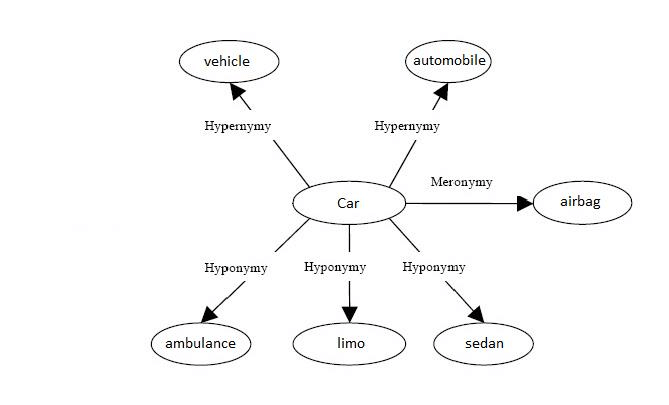
\includegraphics[height=200pt,width=330pt]{img/chapter2/wordnet.jpg}
            \caption{Synset du WordNet de l'Anglais}
            \label{synset}
        \end{figure}
    
    
    \subsection{Plongement de mots (Word embedding)}
    
     \textcolor{red}{Le plongement de mots (word embedding) est une technique qui permet de représenter les mots sous forme d'un vecteur de nombres réels grâce à un apprentissage fait sur un ensemble de mots, ce qui facilite l'anayse sémantique des mots.\\
    Les plongements de mots constituent une méthode pour faire face à un problème récurrent en intelligence artificielle, soit celui de la dimension. En effet, la représentation de mots avec les méthodes traditionnelles (bag of words) représentaient les mots avec un vecteur contenant tout le dictionnaire. En revanche la technique des word embeddings diminue le nombre de ces dimensions, facilitant ainsi les tâches d'apprentissage impliquant ces mots.}
    
    
    \subsubsection{Techniques d'apprentissage}
    
     \textcolor{red}{Il existe principalement deux techniques de word embeddings selon \cite{we1}} :
    
    \begin{itemize}
    \item  \textcolor{red}{La première appelée « Continuous Bag of Words » (CBOW), qui entraîne le réseau de neurones pour prédire un mot en fonction de son contexte, c’est à dire les mots avant/après dans une phrase.\\
    Dans le processus de CBOW, trois couches sont utilisées : la couche d'entrée correspond au contexte, la couche cachée correspond à la projection de chaque mot de la couche d'entrée dans la matrice de poids qui elle même  est projetée sur la troisième couche qui est la couche de sortie.\\ }
   
        \begin{figure}[H]
            \centering
            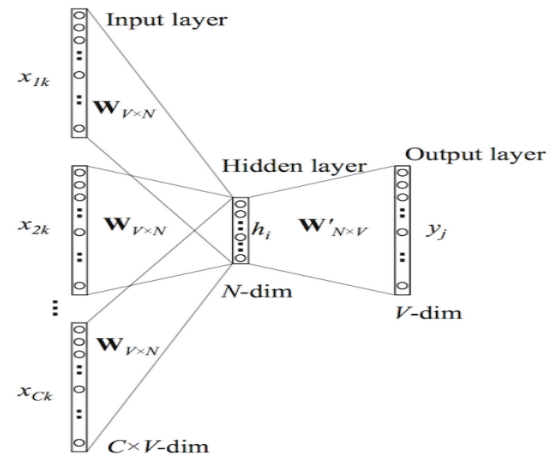
\includegraphics[height=250pt,width=300pt]{img/chapter2/Cbow.png}
            \caption{Réseau de neurones CBOW}
        \end{figure}
        
    
     \item  \textcolor{red}{Dans la seconde méthode, c'est le contraire des modèles CBOW: le modèle essaie de prédire le contexte en fonction du mot. C’est la technique du « skip-gram ». En effet, la couche d'entrée correspond au mot cible
     et la couche de sortie correspond au contexte. Ainsi, Skip-Gram cherche la prédiction du contexte étant donné un mot au lieu de la prédiction d'un mot étant donné son contexte comme c'est le cas pour CBOW.\\}
    
     \begin{figure}[H]
        \centering
        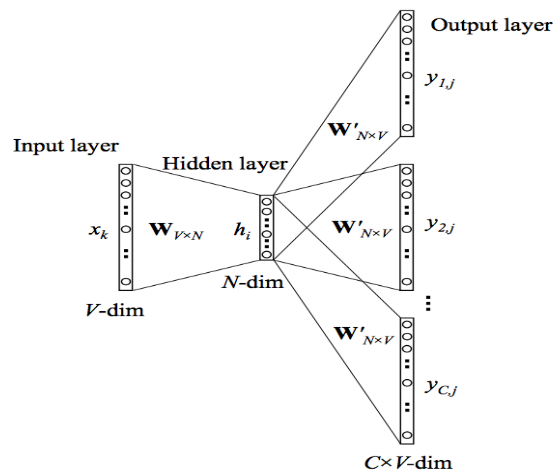
\includegraphics[height=250pt,width=300pt]{img/chapter2/Skip-Gram.png}
        \caption{Réseau de neurones Skip-Gram}
    \end{figure}
    
    \end{itemize}

    \subsubsection{Domaines d'application}
     \textcolor{red}{Grâce au gain en terme de dimensionalité, l'utilisation des plongements de mots (Word embedding) a permis de faciliter la tâche d'apprentissage dans la traduction automatique \cite{we2} en permettant une analyse des bigrammes et trigrammes, ce qui rend la traduction plus contextuelle.\\
    L'analyse des sentiment en a aussi profité, car elle n'a plus besoin de corpus annoté par un expert pour faire l'apprentissage \cite{we3} et la reconnaissance vocale qui a bénéficié d'une réduction des coûts et du temps de collecte et d'annotation de corpus \cite{we4}.}
       
 
    \subsection{Word2Vec}
     \textcolor{red}{Word2vec est un réseau de neurones à deux couches qui traite des documents texte. Son entrée est un corpus de textes et sa sortie est un ensemble de vecteurs: de caractéristiques pour les mots de ce corpus. Bien que Word2vec ne soit pas un réseau de neurones profond, il transforme le texte en une forme numérique que les réseaux profonds peuvent comprendre. Le but et l'utilité de Word2vec est de regrouper les vecteurs de mots similaires dans un espace vectoriel. Autrement dit, il détecte les similitudes mathématiquement. Word2vec crée des vecteurs qui sont des représentations numériques distribuées d'entités de mots, des caractéristiques telles que le contexte de mots individuels; tout cela est fait sans intervention d'un expert.\\}
    
    \subsubsection{Processus d'apprentissage}
    
     \textcolor{red}{Avec suffisamment de données, d'utilisation et de contextes, Word2vec peut faire des prédictions très précises sur la signification d'un mot en fonction des exemples passés. Ces prédictions peuvent être utilisées pour établir l'association d'un mot avec d'autres mots (par exemple, «homme» est un «garçon», «femme» est une «fille»), ou regrouper des documents et les classer par sujet. Ces clusters peuvent constituer la base de la recherche dans le domaine du traitement automatique du langage naturel.\\ 
    La sortie du réseau de neurones Word2vec est un vocabulaire dans lequel chaque élément est associé à un vecteur, qui peut être introduit dans un réseau d'apprentissage en profondeur ou simplement interrogé pour détecter les relations entre les mots. En mesurant la similitude de cosinus, aucune similitude est exprimée sous la forme d'un angle de 90 degrés, alors que la similarité totale de 1 est un angle de 0 degré, un chevauchement complet; c'est-à-dire que Algérie est égale à Algérie, tandis que algérien a une distance cosinus de 0.727976 par rapport à Algérie, qui est la plus petite distance par rapport aux autres mots. Voici une liste de mots associés à "Algeria" en utilisant Word2vec, par ordre de proximité }:
    
    \begin{table}[h!]
        \centering
                 \begin{tabular}{|l|c|r|}
                    \hline
                    Mot & Distance de cosinus\\
                    \hline
                    Algerian & 0.727976 \\
                    Morocco & 0.705196 \\
                    Tunisia & 0.698015 \\
                    Cameroon & 0.651363 \\
                    Gabon & 0.643677 \\ 
                    Algerians & 0.630602 \\
                    Senegal & 0.630219 \\
                    Ivory Coast & 0.627544 \\
                    Angola & 0.620858 \\
                    Burkina Faso & 0.617796 \\
                    \hline
                 \end{tabular}
             \caption{Exemple du vecteur de similarité du mot "Algeria".}
             \label{table:1}
         \end{table}
             
    
    
    
    \subsubsection{Domaines d'application de Word2vec}
     \textcolor{red}{Les applications de Word2vec s'étendent au-delà de l'analyse des phrases. Il peut être appliqué aussi bien aux gènes, au code, aux goûts, aux playlists, aux graphiques de médias sociaux et à d'autres séries verbales ou symboliques dans lesquelles des modèles peuvent être discernés, puisque les mots sont simplement des états discrets comme les autres et nous cherchons simplement les probabilités de transition entre ces états.}
    
    

\section{Résumé automatique}
    \subsection{Définition}
    Le résumé automatique consiste à diminuer le contenu d'un document/texte avec un programme informatique. Le texte résultant (résumé) devrait contenir les idées les plus importantes du texte original.

    \emph{"La synthèse de texte est un processus qui consiste à distiller les informations les plus importantes d'une source pour produire une version abrégée"}\footnote{Traduction par les auteurs de ce mémoire}\cite{aats}(Page 1)\\

    Cette technique est de plus en plus nécessaires pour répondre à la croissance exponentielle des quantités  de données textuelles disponibles sur internet pour mieux reconnaître les informations pertinentes et pour les consommer plus rapidement.

    Dans un livre de 2014 intitulé «Automatic Text Summarization»\cite{atsjmtm}(Pages 4-5), l'auteur à cité 6 raisons pour lesquelles nous avons besoin d'outils pour le résumé automatique:

    \begin{itemize}
        \item Les résumés réduisent le temps de lecture.
        \item Lors de la recherche de documents, les résumés facilitent le processus de sélection.
        \item L'utilisation de cette technique permet d'augmenter le nombre de textes traités.
        \item Le résumé automatique améliore l'efficacité de l'indexation.
        \item Les algorithmes de résumé automatique sont moins biaisés que les synthétiseurs humains.
        \item Les résumés personnalisés sont utiles dans les systèmes de Question/Réponse car ils fournissent des informations personnalisées.
    \end{itemize}

    \subsection{Domaines d'application}    
    Il existe de nombreuses raisons et utilisations des résumés automatiques. Un exemple qui pourrait facilement venir à l'esprit est de créer un résumé d'un article de presse, mais il y a beaucoup plus de cas de résumés de texte que nous pouvons rencontrer tous les jours.

    Voici quelques exemples quotidiens de résumés de textes:
    \begin{itemize}
        \item Grandes lignes (prise de notes)
        \item Synopsis (scénario d'un film)
        \item Avis (Livre, article..)
        \item Biographie (Curriculum Vitae, nécrologie)
        \item Bulletins (prévisions météo)
        \item Histoire (chronologies des événements)
    \end{itemize}

    \subsection{Résumé extractif}
        Cette approche de résumé automatique implique la sélection de phrases à partir d'un document source pour constituer un nouveau texte (résumé). Les techniques consistent à classer la pertinence des phrases afin de retenir celles qui sont les plus importantes pour garder le sens et la signification du texte original.

        La pertinence d'une phrase est calculée à base de plusieurs caractéristiques (Features). Certaines de celles-ci sont\cite{ratsa} :
        
        \begin{itemize}
            \item \textbf{Titre:} Les mots de titre apparaissant dans une phrase pourraient suggérer que la phrase contient des informations importantes
            \item \textbf{Position de la phrase:} Les phrases de début dans un document habituellement décrivent les principales informations concernant document.
            \item \textbf{Longueur de la phrase:} Les phrases trop courtes peuvent contenir moins d'informations et les longues phrases ne sont pas appropriées à représenter le résumé.
            \item \textbf{Poids d'un mot/terme:} Mots ou termes qui ont une occurrence élevée dans un document sont utilisés pour déterminer l'importance d'une phrase.
            \item \textbf{Noms propres/Entités nommées:} les noms de personnes, organisations, lieux, etc. sont considérés comme porteurs d'informations importantes.
        \end{itemize}   

        \subsubsection{État de l'art du Résumé extractif}
        \textbf{•La méthode basée TF-IDF\footnote{Term Frequency-Inverse Document Frequency, méthode de pondération souvent utilisée en recherche d'information.}:}
            Les phrases sont classées en fonction de la fréquence du terme et de l'inverse de la fréquence du document \cite{tfidf}. La similarité entre le vecteur de requête et les vecteurs de phrases est calculée puis les phrases les plus importantes sont incluses dans le résumé. L'inconvénient est  la Redondance dans le résumés.\cite{surveysummarization}
            
        \textbf{•La méthode basée sur apprentissage automatique supervisé:} Les phrases sont classées sur la base de l'inclusion de phrases récapitulatives et de l'exclusion de phrases résumées. La classification est basée sur les caractéristiques de la pertinence des phrases dans le résumé. Les probabilités de classification sont faites sur la base de la technique statistique en utilisant la règle de Bayes. Dans ce cas, la redondance sera peut être réduite mais cette méthode reste complexe.\cite{surveysummarization}
            
        \textbf{•La méthode basée sur le Clustering\footnote{Le partitionnement de données, méthode d'analyse de données, vise à diviser un ensemble de données en différents « paquets » homogènes, chaque sous-ensemble partageant des caractéristiques communes.}:} Ces documents sont représentés en utilisant le TF-IDF de dizaines de mots. La fréquence de terme utilisée dans ce contexte est le nombre moyen d'occurrences (par document) dans le cluster. La valeur IDF est calculée sur la base du corpus entier. Le synthétiseur prend des documents déjà groupés en entrée. Chaque cluster est considéré comme un thème.
        Le thème quant à lui est représenté par des mots avec leurs fréquences d’occurrences.\\
        La sélection de la phrase est basée sur la similarité des phrases au thème du cluster. Le facteur suivant qui est pris en compte pour la sélection de la phrase est l'emplacement de la phrase dans le document (Li). Le dernier facteur qui augmente la score d'une phrase est sa similitude avec la première phrase du document auquel elle appartient (Fi).\\
        L'avantage du clustering est qu'il peut être utilisé pour grouper des phrases similaires dans plusieurs document\cite{surveysummarization}.
            
        \textbf{•La méthode basée Logique Floue\footnote{Formalisée par Lotfi Zadeh en 1965, elle consiste à tenir compte de divers facteurs numériques pour aboutir à une décision qu'on souhaite acceptable.}:} Le système flou considère les caractéristiques des phrases telles que la longueur de la phrase, le mot du titre, les mots-clés, .etc\cite{10}. Il assigne un score aux phrases et extrait les plus importantes sur la base des valeurs assignées.\\
        L'avantage de cette méthode consiste en la facilité de l'extraction des caractéristiques qui servent à calculé le score qui sert, à son tours, comme entrée à \emph{Fuzzifier}, mais la performance de cette approche reste limitée\cite{surveysummarization}.

    \subsection{Résumé abstractif}
        L'approche de résumé automatique abstractive quant à elle, consiste en la génération de phrases entièrement nouvelles. Cette méthode est plus difficile, mais c'est aussi l'approche utilisée par l'humain. Elle est basée sur la sélection et la compression du contenu original.

        Récemment, les méthodes d'apprentissage en profondeur ont montré des résultats prometteurs pour le résumé automatique. Des approches ont été proposées inspirées par l'application de méthodes d'apprentissage en profondeur pour la traduction automatique.

        Principalement basées sur les Réseaux de neurones récurrents, ces dernières ont pu montrer des performances et des résultats assez impressionnants, comme on peut le constater dans \cite{atsuss} et \cite{ruch} où plusieurs nouveaux modèles basés sur l'apprentissage profond ont été proposés qui surpassent statistiquement toutes les autres approches abstractives.

        \subsubsection{État de l'art du Résumé abstractif}
        \textbf{•Méthode basée sur les arbres:} Elle utilise un arbre de dépendance pour représenter le texte d'un document. Sur la base des relations entre les sous-arbres les phrases similaires sont sélectionnées et le résumeur génère le résumé final \cite{5}.
            
        \textbf{•Méthode basée sur un modèle:} Elle utilise un modèle pour représenter le document. Les modèles linguistiques et les règles d'extraction sont utilisées pour identifier les extraits du texte les plus pertinents\cite{5}.

        \textbf{•Méthode basée sur l'ontologie:} Dans cette méthode, \textcolor{red}{il est question d'utiliser des ontologies dans le processus de résumé automatique \cite{ram}.!!}
 
        

\section{Catégorisation de textes}
    \subsection{Définition}
    La catégorisation de textes a pour objectif de regrouper les textes similaires, c'est à dire thématiquement proches. L'intérêt d'une telle démarche est d'organiser les connaissances de façon à pouvoir effectuer, par la suite, une recherche ou une extraction d'information efficace. Elle est largement étudiée dans différentes communautés tels que le Data Mining, les bases de données, l'apprentissage automatique et la recherche d'informations.

    \subsection{Domaines d'application}
    Plusieurs applications dans lesquelles la catégorisation de textes est couramment utilisée, on peut citer:

    \textbf{•Filtrage et organisation des informations d'actualités:} avec les quantités énormes de d'informations d'actualités en ligne, il est très difficile de catégoriser ces dernières manuellement, mais cela est possible grâce aux algorithmes de classifications. 

    \textbf{•Organisation des documents:} aider à la catégorisation de documents, un exemple d'application est l'ensemble des fichiers d'un ordinateur où il s'agit de distinguer les fichiers \emph{log}, \emph{système}, etc.

    \textbf{•Exploration des opinions:} souvent utilisée pour la catégorisation des commentaires sur les réseaux sociaux.

    \textbf{•Catégorisation des emails et filtrage des spams:} reconnaître l'objet de l'email ou déterminer les courriers indésirables de manière automatisée.
     
    \subsection{Technique de classifications de textes}
    De nombreuse techniques ont été conçues pour la catégorisation des textes. Puisqu'il est possible de modéliser ces derniers comme des données quantitatives généralement avec des fréquences de termes, la plupart des méthodes appliquées aux problèmes quantitatifs sont également applicables.\\    
    Quelques une de ces techniques on été citées dans \cite{stca}:

    \begin{itemize}
        \item Arbres de décisions: la division hiérarchique de l'espace de données dans les arbres de décisions permet de créer des partitions de classes qui sont plus asymétriques en termes de distribution de leurs classes.

        \item Base de règles: déterminer les modèles de mots le plus susceptibles d'être liés aux différentes classes, basé sur un ensemble de règles dans lesquelles le coté gauche correspond à un motif de mot, et le coté droit à une étiquette de classe.

        \item SVM: tentent de partitionner l'espace de données en utilisant des fonctions linéaires et non linéaires pour séparer les classes.

        \item Réseau de neurones: avec l'utilisation des caractéristiques des mots, tout comme les SVMs les RNs essaient de trouver la limite la plus optimale entre les classes.

        \item Autres: presque tous les algorithmes de classification peuvent être adaptés aux données textuelles, tel que les algorithmes génétiques, etc.
    \end{itemize}


    \subsection{Catégorisation d'articles de presse}
     L’étude de la presse en ligne est devenue ces derniers temps un enjeu de recherche, et le nombre phénoménal de journaux, magazines et blogs sur internet qui ne cessent d'augmenter a fait de la catégorisation d'articles de presse l'une des tâches les plus importantes de la catégorisation de textes. Il s'agit de ranger des articles dans des classes, idéalement convenables, suivant une problématique donnée, souvent le domaine traité par l'article, comme Politique, Sport, Religion, Économie, etc.

    \subsubsection{État de l'art de la catégorisation d'articles de presse}
    
      \textcolor{red}{De nombreux travaux de recherches ont été faits dans la catégorisation de textes mais ce qui est plus intéressant pour nous c'est de prospecter ceux destinés à la catégorisation des articles de presse \cite{itemetat0}, parmi ceux-là on retrouve} :
     
     \begin{itemize}
        
     \item  \textcolor{red}{Thorsten Joachims introduit les machines à vecteurs de support (Support vector machine) pour la catégorisation de textes. Il fournit à la fois théorique et preuve empirique que les SVM sont très bien adaptés pour la catégorisation de textes \cite{itemetat1}}. 
     
     \item  \textcolor{red}{Susain Dumais compare l'efficacité de cinq algorithmes d'apprentissage automatique différents pour la catégorisation en termes de vitesse d'apprentissage, classement en temps réel, la vitesse et la précision de la classification. Il examine également la taille de l'ensemble d'entraînement et la représentation de documents alternatifs \cite{itemetat2}}.
     
     \item  \textcolor{red}{Chee Hong a expérimenté une approche automatisée pour classer les articles de presse en ligne en utilisant la méthode de classification SVM. L'utilisation de SVM a donné de bons résultats quand les données d'apprentissage (Articles de presse) étaient suffisants \cite{itemetat3}}.
      
     \item  \textcolor{red}{Krishanalal a développé le classifieur d'articles de presse intelligent et l'à expérimenté en ligne pour les catégories Sports, Finances et politique. L'approche novatrice combinant deux puissants algorithmes, modèle de Markov caché et SVM, dans le domaine de classement en ligne des articles de presse a fourni de bons résultats par rapport aux méthodologies existantes. Par l'introduction de plusieurs techniques de prétraitement, ils ont pu améliorer la précision du classifieur \cite{itemetat6}}.
     
     \item  \textcolor{red}{Mita K. Dalal a travaillé sur la classification de textes et l'extraction des caractéristiques; il a conclu que les étapes de pré-traitement et de sélection des fonctions ainsi que le choix des données d'apprentissage jouent un rôle crucial dans pour l'amélioration de la précision \cite{itemetat7}}. 
     
     \item  \textcolor{red}{Adgar a proposé une approche pour classer les articles de presse et l'a décomposée en 3 étapes: prétraitement du texte, extraction de caractéristiques basée sur TF-IDF et la classifiation basée sur SVM.
     Il a choisi SVM, car ceux-ci peuvent supporter données avec des dimensions élevées \cite{itemetat8}}.
     
     \end{itemize}
        

\section{La traduction automatique}
La traduction est une activité en croissance très rapide de nos jours \cite{tradstat}. C'est un moyen actif de transférer la culture et la langue en communicant avec autrui \cite{tradcom}. Son aspect principal est de faire passer un message ou un texte rédigé d'une langue vers une autre en respectant le contexte et la grammaire.\\
Depuis très longtemps, la traduction automatique s'inscrit dans une recherche appartenant au domaine du traitement automatique du langage naturel.
    \subsection{Définition}
    La traduction automatique est la procédure par laquelle un ordinateur évalue un contenu source en entrée dans une langue donnée et délivre un contenu cible dans une langue différente en respectant les aspects lexicaux, syntaxiques, sémantiques et morphologiques des deux langues.
    \subsection{Types de traduction automatique}
    Les traducteurs automatiques se distinguent dans les catégories suivantes en :
        \subsubsection{Traducteur automatique basé dictionnaire}
        Dans ce type de traducteur, historiquement l'approche la plus ancienne et obsolète, la traduction automatique était basée sur les traductions des dictionnaires multilingues ordinaires, c'est a dire la traduction des mots du texte en entrée mot par mot en ne prenant pas en considération le sens des phrases. Il est a noter que les recherches dans le dictionnaire peuvent être faites avec ou sans l'utilisation des outils de langages dans l'analyse.
        \subsubsection{Traducteur automatique à base de règles de production}
        Dans ce type de traduction automatique, le traducteur prend en compte les données étymologiques des langues des documents en entrée et le document cible fondamentalement récupéré de 
        lexiques et structures de phrases couvrant les règles sémantiques, morphologiques et syntaxiques principales de chaque langue individuellement. L'acquisition des phrases composant la langue du document source par le traducteur permet de produire des phrases cibles dans la langue du document cible sur le principe d'analyses morphologique, syntaxique et sémantique des deux langues.
        Les principaux travaux utilisant les bases de règles pour la traduction ont été créés au milieu des années 1970\cite{surveyTraduction}.
        Les traducteurs automatiques à base de règles de production sont capables de produire des traductions avec une qualité raisonnable, mais la construction du système prend beaucoup de temps et de main-d'œuvre parce que ces ressources linguistiques doivent être fabriquées à la main.De plus, il est très difficile de corriger l'entrée ou d'ajouter de nouvelles règles au système pour générer une traduction\cite{jean}.
        \subsubsection{Traducteur automatique à base d'exemples}
        L'approche à base d'exemples repose sur un ensemble de phrases traduites préalablement. Lors de la traduction, le processus vérifie si la phrase à l'entrée est parmi les exemples; dans le cas positif, il fournit directement sa traduction, sinon il s'inspire d'autres phrases contenant un ou plusieurs ensembles de mots similaires et fournit la traduction de ces mots selon les exemples dont il dispose\cite{gent}.
        \subsubsection{Traducteur automatique basé connaissances}
        Ce type de traducteur automatique se concentre sur l'aspect lexical que représente un domaine défini (propre à un seul domaine), comme par exemple, un traducteur pour les articles de recherches, médecine, etc\cite{surveyTraduction}.
        \subsubsection{Traducteur automatique basé sur un corpus}
        La traduction automatique basée sur le corpus (CBMT) est générée sur l'analyse des corpus de textes bilingues. Cette technique utilisée depuis 1989 se base sur un corpus de traduction pour la machine. Cette technique a dominé sur les autres compte tenu de son exactitude, notamment à l'ajout d'exemples au système qui peut améliorer ses performances puisqu'il est basé sur les données, bien que l'accumulation et la gestion de l'énorme corpus de données bilingues puisse également être coûteuses\cite{jean}.
        \subsubsection{Traducteur automatique basé contexte}
        La traduction automatique basée contexte est un nouveau paradigme pour la traduction automatique basée corpus qui nécessite un vaste corpus de textes cibles monolingues et un dictionnaire bilingue complet. CONTRAST \cite{8} et REFTEX \cite{9} sont deux exemples de systèmes de traduction automatique basée contexte.


\section{Conclusion}
Dans ce chapitre, nous avons essayé de faire le tour des techniques du Traitement Automatique du Langage Naturel. Nous avons d'abord présenté cette science, son importance et ses domaines d'application. Ensuite, nous avons examiné l'état de l'art de chaque technique en expliquant les processus et les méthodes. Enfin, nous avons passée rapidement en revue certaines applications actuelles du TALN.
Le prochain point à aborder quant à lui, présentera notre contribution, la conception générale de la solution proposée et ses différentes fonctionnalités.  

\chapter{Conception}    
%!TEX program=luatex

\newpage
\section{Introduction}
La réalisation d'un logiciel ou d'un système informatique doit être obligatoirement précédée d'une étape d'analyse et de conception qui a pour objectif de définir et de formaliser les étapes nécessaires du développement de l'application afin de rendre cette dernière plus fidèle aux besoins.

La première motivation de ce travail été de fournir un outil qui permet à l'utilisateur de faire ça revue de presse quotidienne de la façon la plus efficace et la plus enrichissante possible tout en considérant ses centres d'intérêt et préférences. 

Le logiciel que nous proposons enchaîne les processus de catégorisation, de résumé, de traduction et de recommandation d'articles de presse. Pour parvenir à réaliser cet ensemble de tâches en deux langues (Anglais et Arabe), nous allons présenter dans cette partie notre conception qui décrit d'une manière claire et précise le fonctionnement de chaque module du système. 


\section{Module de recommandation}
Dans cette partie, nous allons voir la conception détaillée de notre système de recommandation. Ci-dessous, nous présentons les deux approches proposées, la recommandation personnalisée et non-personnalisée d'articles de presse.
    \subsection{Recommandation personnalisée\label{personal}}
    La recommandation d'articles est basée sur le contenu des profils utilisateurs. En effet, le profilage débute lorsque l'utilisateur s'authentifie pour la première fois et à chaque fois les informations relatives à ses préférences sont récoltées et traitées.

    Cette étape nécessite le profilage des utilisateurs et le calcul de similarité entre ces derniers. Dans ce qui suit les détails de chacune des deux méthodes.

        \subsubsection{Profilage d'un utilisateur}
        Elle consiste à déterminer les centres d'intérêt d'un utilisateur tout en se basant sur les articles lus et visiter. Pour cela, nous avons mis en place plusieurs méthodes de calcul des probabilités de préférences afin de mieux cibler les utilisateurs et garantir une solution conforme aux caractéristiques de la recommandation pour les articles de presse. 

        Pour le calcul des probabilités de préférences utilisateurs, nous avons utilisé une méthode de calcul qui permet à la fois de résoudre le problème de la récence \autoref{} et le démarrage à froid \autoref{}. Cette méthode testée s'avère très efficace par rapport aux méthodes existantes et décrites dans \autoref{}.

        Le calcul de la probabilité de sélection d'une catégorie pour un utilisateur est basé sur ses interactions avec les articles de presse disponible. Dés qu'un article est sélectionné, l'information est sauvegardée et utilisée pour la mise à jour du vecteur des probabilités de sélection des catégories préférées \autoref{}.

        L'exemple suivant présente un vecteur de probabilité de sélection pour les catégories préférées d'un utilisateur U :
            \[P(U) = {'sport': 0.7178, 'news': 0.1581, 'sci\_tech': 0.1492}\]            
        Il faut noter que la taille du vecteur de probabilité de sélection des catégories préférées est différentes d'un utilisateur à un autre.

        Ce vecteur se met à jour, comme déjà cité, après chaque interaction de l'utilisateur U avec l'article A de la catégorie C. Au fur et à mesure, la probabilité de sélection d'une catégorie C\textsubscript{i} augmente si cette dernière est sélectionnée, sinon, elle diminue pour donner moins d'importances aux articles qui font partie de cette catégorie.

        Ci-après les formules dédiées à la mise à jour des probabilités de sélection des catégories préférées :\\
            \[
            P(U, C) =
            \begin{cases}
                (1-{\alpha}) * {P(U, C)} + {\alpha} & \text{si } \text{article A est sélectionné} \\
                (1-{\alpha}) * {P(U, C)} & \text{sinon.}
            \end{cases}
            \]

        Avec initialement :\\
        \[
        \begin{cases}
            P(U, C) = 1 / \text{NbC } \forall \text{ C} \in \{categorie\textsubscript{1}, categorie\textsubscript{2}, ..., categorie\textsubscript{NbC}\}\\
            NbC : \text{nombre de categories}\\
            \alpha = \text{constante empirique représentant le biais de la diminution}
        \end{cases}
        \]
        \begin{algorithm2e}[H]
        \SetAlgoLined
        \SetKwInOut{Input}{input}
        \SetKwInOut{Output}{output}
        \Input{A: Article, U: Utilisateur}
        \textbf{const :} \alpha = 0.1, NbC = nombre de catégories\\
        préférences = U.préférences\\
        catégorie = A.catégorie\\
        \eIf{catégorie \in préférences}{
            préférences[catégorie] = (1-{\alpha}) * {préférences[catégorie]} + {\alpha}\\
            \While{i < taille(préférences)}{
                \If{préférences[i] != catégorie}{
                    préférences[i] = (1-{\alpha}) * {préférences[catégorie]}\\
                }
            } 
        }
        {
            préférences[catégorie] = 1 / NbC
        }
        \caption{Algorithme de profilage d'un utilisateur}
        \end{algorithm2e}
        \subsubsection{Similarité entre utilisateurs}
        Afin de diversifier la recommandation d'articles de presse, nous avons mis en place une méthode de calcul de similarité entre utilisateur qui permet de recommander des articles selon les préférences et les centres d'intérêt d'un utilisateur similaire. 

        Selon \cite{euclidepreuve} qui propose une étude détaillée sur les mesures de similarité pour le filtrage collaboratif, il en est ressorti comme conclusion que la distance euclidienne était la mesure la plus adéquate en terme de précision et temps d'exécution. La formule de calcul de la distance euclidienne entre les préférences des utilisateurs est la suivante :

        \begin{itemize}[label={}, leftmargin=0cm]
            \item Soient U\textsubscript{1} et U\textsubscript{2} deux utilisateurs,
            \item P(U\textsubscript{1}) et P(U\textsubscript{2}) les vecteurs de probabilité de sélection des catégories préférées des deux utilisateurs respectivement,
            \item NbC\textsubscript{1} et NbC\textsubscript{2} le nombre de catégories préférées de chaque utilisateur,\  
            \item \[Sim({P(U\textsubscript{1})}, {P(U\textsubscript{2})}) = d({P(U\textsubscript{1})}, {P(U\textsubscript{2})}) = {\sqrt {\sum _{i=1, j=1}^{NbC\textsubscript{1},NbC\textsubscript{2}}(P(U\textsubscript{1}, C\textsubscript{i})-P(U\textsubscript{2}, C\textsubscript{j}))^{2}}}\]
        \end{itemize}

        Dans ce qui suit, un exemple de calcul de similarité entre deux utilisateurs :
        \[
        \begin{cases}
            P(U\textsubscript{1}) = {'sport': 0.7581, 'sci\_tech': 0.4492, 'religion': 0.3878, 'algeria': 0.0178,}\\
            P(U\textsubscript{2}) = {'religion': 0.8813,'sport': 0.4421, 'business': 0.3519}\\
        \end{cases}
        \]
        On ignore les probabilités de sélection des catégories non-commune entre les deux utilisateurs.
        \[
        \begin{cases}
        d({'sport'}) = P(U\textsubscript{1},'sport')-P(U\textsubscript{2},'sport') = 0.7581 - 0.4421 = 0.32\\
        d({'religion'}) = P(U\textsubscript{1},'religion')-P(U\textsubscript{2},'religion') = 0.3878 - 0.8813 = −0,49 \\
        Sim({P(U\textsubscript{1})}, {P(U\textsubscript{2})}) = {\sqrt {d({'sport'})^{2}+d({'religion'})^{2}}}= {\sqrt{(0.32)^{2} + (-0.49)^{2}}} = 0,59
        \end{cases}
        \]
        \begin{algorithm2e}[H]
        \SetAlgoLined
        \SetKwInOut{Input}{input}
        \SetKwInOut{Output}{output}
        \Input{A: Article, U: utilisateur}
        \textbf{const :} seuil = 0.1\\
        utilisateurs = Lire(collection de profils)\\
        \While{i < taille(utilisateurs)}{
            \If{utilisateurs[i] != U}{
                sim = distance\_euclidienne(U.préférences, utilisateurs[i].préférences)\\
                \If{sim >= seuil}{
                    U.préférences += utilisateurs[i].préférences
                }
            }
        } 
        \caption{Algorithme de calcul de similarité entre utilisateurs}
        \end{algorithm2e}

    \subsection{Recommandation non-personnalisée}
    La recommandation non-personnalisée vise à recommander des articles pour des utilisateurs qui n'ont pas de comptes (i.e : qui sont non authentifiés), pour cela, notre système effectue une recommandation selon le choix de lecture de l'utilisateur, c'est-à-dire par calcul de similarité entre l'article qui est en train d'être lu et les nouveaux articles disponibles. 

    Un pré-traitement est effectué sur chaque article comprend la suppression des mots vides et l'extraction des racines de mots. Ensuite, le sac à mots (Bag of Words) de l'article est converti en TF-IDF. La matrice résultante de la conversion en TF-IDF est utilisée pour le calcul de la similarité de cosinus et les cinq articles les plus similaires seront recommandés. Le calcul de la similarité entre les articles est présenté ci-dessous.

    \begin{itemize}[label={}, leftmargin=0cm]
        \item Soient U un utilisateur, A\textsubscript{1} et A\textsubscript{2} deux articles de presse,
        \item A\textsubscript{1} a été déjà sélectionné et A\textsubscript{2} est un nouvel article,
        \item BoW(A\textsubscript{1}) et BoW(A\textsubscript{2}) les sacs à mots de chaque article,\\

        \item BoW(A\textsubscript{1}) = \{\begin{arab}'لواء', 'شفيق', 'مدير', 'مكتب', 'رئيس', 'مخلوع', 'مبارك', 'أراد', 'دائم', 'إيقاع', 'عمر', 'سليمان', 'مشير', 'طنطاوي', 'وصف', 'لواء', 'شفيق', 'عاش', 'قصر', 'رئيس', 'مصري', 'مخلوع', 'وفاة', 'عمر', 'سليمان', 'رئيس', 'مخابرة', 'مصري', 'نائب', 'مبارك', 'خسارة', 'أكبر', 'مصر', 'رجل', 'أفضل', 'رجل', 'شجع', 'صعب', 'تعويض', 'تحدث', 'لواء', 'شفيق', 'تصريح', 'علاقة', 'عمر', 'سليمان', 'رئيس', 'مخلوع', 'مبارك'\end{arab}\},

        \item BoW(A\textsubscript{2}) = \{\begin{arab}'استمر' 'نزاع', 'رئيس', 'وزير', 'نوري', 'مالكي', 'شيعي', 'خصم', 'حكم', 'أنصار', 'قائمة', 'عراقي', 'لواء', 'خلفية', 'اتهام', 'مالكي', 'نائب', 'رئيس', 'طارق', 'هاشمي', 'شجع', 'ضلع', 'عملية', 'إرهابي', 'أمر', 'أدى', 'تجميد', 'نشاط', 'حكومة', 'انسحاب', 'وزير', 'قائمة', 'عراقي', 'تفاقم', 'خلاف', 'نظر', 'مطالبة', 'تيار', 'رجل', 'صدري', 'قائمة', 'عراقي', 'علاقة', 'حل', 'برلمان'\end{arab}\},


        \item TF-IDF(A\textsubscript{1}) = \{0.0766346 , 0.05452615 , 0.4598076 , 0.1090523,  0.076346, 0.0766346, 0.0766346, 0.1090523, 0.16357845, ...\},

        \item TF-IDF(A\textsubscript{2}) = \{0.0261347 , 0.156338 , 0.229038 , 0.0730857,  0.0520013, 0.0816399, 0.0261347, 0.2299038, 0.16357845, ...\},

        \item \[sim\_cos(TF-IDF(A\textsubscript{1}), TF-IDF(A\textsubscript{2})) = \frac {TF-IDF(A\textsubscript{1}) \cdot TF-IDF(A\textsubscript{2})}{||TF-IDF(A\textsubscript{1})|| \cdot ||TF-IDF(A\textsubscript{2})||}\]
    \end{itemize}
    \begin{algorithm2e}[H]
        \SetAlgoLined
        \SetKwInOut{Input}{input}
        \SetKwInOut{Output}{output}
        \Input{A: Article, U: utilisateur}
        \Output{ListeArticlesSimilaires: Article}
        articles = Lire(collection d'articles)\\
        \While{i < taille(articles)}{
            segmentation(articles[i])\\
            suppression\_mots\_vides(articles[i])\\
            racinisation(articles[i])\\
        }
        tf-idf = TF-IDF(articles)\\
        mat\_similarité = Tri(cosinus\_similarité(tf-idf))\\
        ListeArticlesSimilaires = mat\_similarité.articles\\
        \Return ListeArticlesSimilaires[:5]
        \caption{Algorithme de calcul de similarité entre articles}
    \end{algorithm2e}

%%~~~~~~~~~~~~~~~~~~~~~~~~~~~~~~~~~~~~~~~~~~~~~~~~~~~~~~~~~~~~~~~~~~~~~~~~~~~~~~~~~~~~~~~~~~~~~~~~~%%
\section{Module de catégorisation d'article de presse}
Le premier module sur lequel nous avons travailler, c'est la catégorisation d'articles de presse. Nous avons expérimenter plusieurs techniques proposées dans la littérature. Nous présentons ci-après chaque approche, ses résultats, ses points forts et ses faiblesses.

% En se basant sur les travaux de \cite{categorisation} pour l'Anglais et \cite{categorisation} pour l'Arabe, nous avons entraîné nos modèles sur des corpus d'articles de différentes sources afin de garantir la diversité dans nos données (plus de détails dans le chapitre 4\ref{chapter4}).
% À REVOIR!!

    \subsection{Approches expérimentées\label{approches}}
    Toutes les approches utilisées, pour la catégorisation d'articles de presse, sont basées sur l'apprentissage automatique, supervisé et non supervisé. 

    \subsubsection{Basées sur l'Apprentissage Non Supervisé}
        \begin{itemize}
            \item{LDA (Latent Dirichlet Allocation) : }\\
            "Latent Dirichlet Allocation" est un modèle probabiliste génératif qui permet de décrire des collections de documents de texte ou d'autres types de données discrètes. LDA fait partie d'une catégorie de modèles appelés "topic models", qui cherchent à découvrir des structures thématiques cachées dans des vastes archives de documents. L'organisation automatique des documents par sujet est une application connue de LDA.
        \end{itemize}
        
    \begin{itemize}[label={}, leftmargin=*]
        \item{\textbf{Corpus et dataset}}\\
        Le Dataset \emph{DeepMind Q\&A} de Hermann et al. (2015) \cite{cnndailymail} a été utilisé. Les articles de presse ont étaient récoltés pour l'utilisation dans un travail de recherche dans les systèmes de Questions/Réponses. Le corpus est contient 92 579 articles de presse de \emph{CNN}.

        Chaque article est sous le format suivant :
       \begin{itemize}
        \item \textbf{id : }identifiant unique de l'article.
        \item \textbf{contenu : }contenu de l'article.
       \end{itemize}
    \end{itemize}
        
    \subsubsection{Basées sur l'Apprentissage Supervisé}
        \begin{itemize}
            \item{Naïve de Bayes : }\\
            C'est une méthode connue de l'apprentissage automatique supervisé. Un de ses avantages, en plus d'être un modèle simple et facilement interprétable, c'est qu'il renvoie le degré de certitude en plus de la prédiction, ce qui peut être très utile dans certaines applications. 

            Mais en ayant un problème à classes multiples, cette approche nous a donnés des résultats très modeste en un temps d'exécution assez importants, ce qui nous a poussé à abandonner son utilisation.\\
            
            \item{Arbres de décision : }\\
            L'un des algorithmes d'apprentissage automatique supervisé les plus facile à interpréter. Ces principaux avantages sont : robuste face aux données aberrantes, pas très sensible aux données manquantes, possibilité d'intervenir dans la construction de l'arbre, etc. 

            Son principale inconvénient reste la dépendance très forte entre la taille de la base d'apprentissage et les performances.\\
            
            \item{SVM (Support Vector Machines) : }\\
            Les machines à vecteurs supports (en anglais Support Vector Machine, SVM) sont destinées à résoudre des problèmes de classification et de régression. Les SVMs cherchent à trouver la frontière séparatrice optimale entre les classes, à partir d'un ensemble d'apprentissages. Dans le cas de la classification de textes (articles de presse dans notre cas), les SVMs ont montrés une grande capacité de prédiction malgré le très grand nombre de caractéristiques des textes (> 10000) contrairement aux autres techniques.\\ 
            
            \item{Descente de Gradient Stochastique : }\\
            Le SGD est un algorithme de classification linéaire, souvent utilisé pour l'optimisation. Il peut être combiné avec d'autres techniques d'apprentissage, (SVM, Réseau de neurones, etc.), comme  fonction d'optimisation d'erreur. Dans notre cas, il est utilisé avec un SVM pour le modèle de catégorisation d'articles de presse arabe.
        \end{itemize}

    \begin{itemize}[leftmargin=*, label={}]
        \item{Corpus et dataset}\\
            Nous avons défini une structure pour chaque article, pour faciliter l'exploration des datasets. Ci-dessous la structure choisie :
            \begin{itemize}
               \item{\textbf{id} : }un identifiant unique de l'article,
               \item{\textbf{contenu} : }les différents paragraphes de l'article,
               \item{\textbf{catégorie} : }la catégorie de l'article extraite depuis la source.
            \end{itemize}
    \end{itemize}

    \subsection{Processus de catégorisation}
        \subsubsection{Pré-traitement des articles de presse}\label{pretraitement}
        Plusieurs opérations de pré-traitements ont été effectuées sur chaque article dans le but de rendre l'utilisation des données avec les différents algorithmes d'apprentissage automatique possible.

        On prend le paragraphe suivant comme exemple :

            \begin{arab}أمرت السلطات القطرية الأسواق والمراكز التجارية في البلاد برفع وإزالة السلع الواردة من السعودية والبحرين والإمارات ومصر في الذكرى الأولى لإعلان هذه الدول الحصار عليها.\end{arab}
            
        Ci-après les étapes de pré-traitement suivies :
        \begin{enumerate}[leftmargin=*]
            \item{\textbf{Segmentation (Tokenization) et suppression des mots vides :} }permet d'extraire toutes les entités lexicales d'un article donné. La segmentation est suivie de la suppression des tokens non-utiles tel que la ponctuation, les pronoms, les déterminants, etc.

            Après segmentation : \{
                \begin{arab}'أمرت', 'السلطات', 'القطرية', 'الأسواق', 'و', 'المراكز', 'التجارية', 'في', 'البلاد', 'برفع', 'و', 'إزالة', 'السلع', 'الواردة', 'من', 'السعودية', 'و', 'البحرين', 'و', 'الإمارات', 'و', 'مصر', 'في', 'الذكرى', 'الأولى', 'لإعلان', 'هذه', 'الدول', 'الحصار', 'عليها', '.'\end{arab}
            \}

            Après suppression des mots vides : \{
            \begin{arab}'أمرت', 'السلطات', 'القطرية', 'الأسواق', 'المراكز', 'التجارية', 'البلاد', 'برفع', 'إزالة', 'السلع', 'الواردة', 'السعودية', 'البحرين', 'الإمارات', 'مصر', 'الذكرى', 'الأولى', 'لإعلان', 'الدول', 'الحصار'\end{arab}
            \}\\
            
            \item{\textbf{Racinisation (Stemming) :} }les mots d'un document sont représentés par leurs racines plutôt que par les mots d'origine. Plusieurs variantes d'un terme peuvent ainsi être groupées dans une seule forme représentative, ce qui réduit le nombre des termes distincts nécessaires pour représenter un document.

            Après racinisation : \{
            \begin{arab}'أمر', ' سلطة ', 'قطر', 'سوق', 'مركز', 'تجاري', 'بلد', 'رفع', 'إزالة', 'سلعة', 'وارد', 'سعودية', 'بحرين', 'إمارة', 'مصر', 'ذكرى', 'أول', 'إعلان', 'دولة', 'حصار'\end{arab}
            \}\\

            \item{\textbf{N-grammes :} }les N-grammes permettent de construire une sous-séquence de n mots consécutifs. Ils permettent de contextualiser l'ordre d'apparition d'un ensemble de mots.

            Après génération des N-grammes (bi-grammes dans notre cas) : \{
            \begin{arab}('أمر', 'سلطة'), ('سلطة', 'قطر'), ('قطر', 'سوق'), ('سوق', 'مركز'), ('مركز', 'تجاري'), ('تجاري', 'بلد'), ('بلد', 'رفع'), ('رفع', 'إزالة'),('إزالة', 'سلعة'), ('سلعة', 'وارد'), ('وارد', 'سعودية'), ('سعودية', 'بحرين'), ('بحرين', 'إمارة'), ('إمارة', 'مصر'), ('مصر', 'ذكرى'), ('ذكرى', 'أول'), ('أول', 'إعلان'), ('إعلان', 'دولة'), ('دولة', 'حصار')\end{arab}
            \}\\
        \end{enumerate}
        \subsubsection{Modèle de classification d'articles de presse}
            Nous avons développé plusieurs modèles de catégorisation d'articles de presse basés sur l'apprentissage supervisé et non supervisé cités présentés la \autoref{approches}. L'algorithme \autoref{algomodeles} présente les étapes de développement des différents modèles.

            \begin{algorithm2e}[H]
            \label{algomodeles}
            \SetAlgoLined
            \SetKwInOut{Input}{input}
            \SetKwInOut{Output}{output}
            \Input{Dataset: Article}
            \Output{ModèleEntrainé}
            tf-idf = [ ]\\
            \For{article \in Dataset}{
                segmentation(article)\\
                suppression\_mots\_vides(article)\\
                racinisation(article)\\
                n-grammes(article)\\
                tf-idf += TF-IDF(article)
            }
            ModèleEntrainé = AlgorithmeClassification(tf-idf)\\
            \Return{ModèleEntrainé}
            \caption{Algorithme de construction des modèles de catégorisation}
            \end{algorithm2e}

        \subsubsection{Prédiction des catégories d'articles de presse}
            Une fois le modèle est prêt, nous utilisons le résultat pour la prédiction d'un nouvel article. L'article à classifier doit passé par les mêmes étapes de pré-traitement cités dans la \autoref{pretraitement}. On peut voir le processus de la prédiction dans l'algorithme \autoref{algoprediction}.

            \begin{algorithm2e}[H]
            \label{algoprediction}
            \SetAlgoLined
            \SetKwInOut{Input}{input}
            \SetKwInOut{Output}{output}
            \Input{A: Article}
            \Output{catégorie: Catégorie}
            segmentation(A)\\
            suppression\_mots\_vides(A)\\
            racinisation(A)\\
            n-grammes(A)\\
            prédiction = Charger(modèle)
            catégorie = prédiction(A)
            \Return{catégorie}
            \caption{Algorithme de prédiction de catégorie d'un article de presse}
            \end{algorithm2e}
%%~~~~~~~~~~~~~~~~~~~~~~~~~~~~~~~~~~~~~~~~~~~~~~~~~~~~~~~~~~~~~~~~~~~~~~~~~~~~~~~~~~~~~~~~~~~~~~~~~%%

\section{Module de résumé automatique}
Pour ce module de résumé automatique, nous avons choisi un résumeur automatique extractif \cite{notreresume} basé sur les plongements de mots (Word embeddings)!!!!!!! comme décrit dans le chapitre précédent \autoref{}.
Ci-dessous la présentation des différentes approches expérimentées.
    \subsection{Résumé extractif par Apprentissage Supervisé}
    Nous avons, tout d'abord, expérimenté l'approche proposé dans \ref{riad-belkbir} qui est basée sur un apprentissage automatique supervisé en utilisant un dataset annoté manuellement. 
        \subsubsection{Corpus et datasets}
        Le dataset contient plus de 70 articles. Il est dédié principalement au résumé automatique par apprentissage supervisé pour la langue Arabe, mais peut être utilisé également dans d'autres applications, telles que la compression des textes.

        L'annotation consiste en l'attribution de quatre type d'étiquettes possibles à chaque phrase de l'article :
            \begin{itemize}
                \item S (select) : phrase importante, à prendre en considération dans la construction du résumé.
                \item R (remove) : cette phrase est à supprimer, son absence n'affecte pas le sens du résumé.
                \item F (fusion) : fusion de deux phrases (ou plus).
                \item C (compress) : compression d'une phrase on supprimant les synonymes et les redondances dans le sens.\\
            \end{itemize}

        \subsubsection{Pré-traitement et structure du dataset}
        Tout les articles du dataset sont sous le format XML, chaque article a son propre identifiant et divisé en paquets de phrases selon l'opération effectuée. Ci-après la \autoref{xml-structure} qui montre un exemple du dataset : 
        \begin{figure}[H]
            \centering
            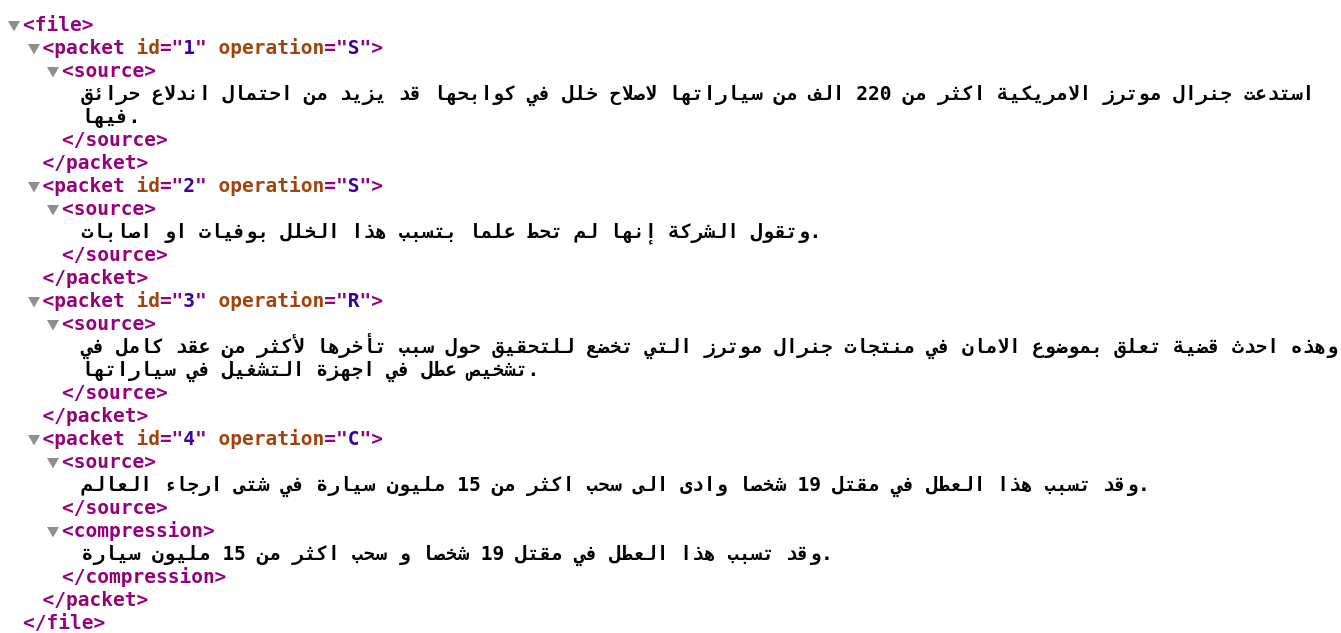
\includegraphics[height=220pt,width=430pt]{img/chapter4/xml.png}
            \caption{Structure d'un article du dataset de résumé automatique}
            \label{xml-structure}
        \end{figure}
        L'approche basée sur l'apprentissage automatique demandait un très grand nombre d'articles résumés, ce qui nous a poussé à l'abandonner.

    \subsection{Résumé extractif par Machine de Boltzman}
    L'approche proposée dans \cite{boltzman} utilise un modèle d'apprentissage profond afin de prédire les phrases les plus importantes dans un texte donnée en utilisant 9 caractéristiques sur chaque phrase. Elle consiste en trois grande phases: l'extraction des caractéristiques, la conversion en valeurs numériques et la génération du résumé à partir des scores de chaque phrase. 

    Les caractéristiques extraites sont les suivantes :
    \begin{enumerate}
        \item{Nombre de mots clés}
        \item{Position de la phrase dans le texte}
        \item{Longueur de la phrase}
        \item{Position de la phrase dans le paragraphe}
        \item{Nombre de noms propres}
        \item{Nombre d'entités numériques}
        \item{Nombre d'entités nommées}
        \item{TF-ISF (Term Frequency- Inverse Sentence Frequency)}
        \item{Similarité avec la phrase centroïde}
    \end{enumerate} 

    \subsection{Résumé automatique extractif par Plongement de mots\ref{plongement}}
    L'approche proposée par l'équipe de recherche du département informatique de l'Université de Bari en Italie \cite{bari}, est basée sur la similarité textuelle entre la phrase centroïde et les autres phrases du texte en utilisant les plongements de mots (Word embeddings)\ref{}. Le plongement de mots utilisé dans cette approche est un modéle skip-gram entrainé sur le contenu de Wikipédia \cite{} en utilisant la bibliothèque fasttext du laboratoire en intelligence artificielle de facebook qui ont dévellopé des modéles pour 294 langues différentes \cite{fasttext}. parmi les modéles developpé, nous allons nous intérésser a celui de l'anglais et l'arabe. La conception et l'algorithme de réalisation sont détaillés dans \ref{plongement}. Ci-dessous, nous allons présenter les étapes de conception du résumé automatique.

        \subsubsection{Prétraitement des articles}
        Dans cette phase, il suffit juste de segmenter le texte, le tokeniser et supprimer les mots vides. Ceci étant dû au fait que le plongement de mots que nous allons utiliser (le modèle Skip-Gram entraîné sur le contenu Wikipédia) servira entre autre a détecter les régularités linguistiques des  mots de la même racine. par exemple : le mot le plus similaire a "Algeria" est le mot "Algerian" \ref{}, c'est pour cela que le stemming n'est pas utilisé dans ce cas.

         \begin{algorithm2e}[H]
           \SetAlgoLined
          \SetKwInOut{Input}{input}
          \SetKwInOut{Output}{output}
          \Input{A: Article}
          \Output{ListeTokens: token}
          Lire(A)\\
          phrases = segmentation(A)\\
          \For{phrase \in phrases}{
            tokens = tokenisation(phrase)\\
            ListesTokens += suppression\_mots\_vides(tokens)\\
          }
          \Return {ListesTokens}
         \caption{Algorithme de prétraitment du résumé}
        \end{algorithm2e}

       \subsubsection{Construction d'un vecteur de centroïde}
        Après l'étape de prétraitement, place a la construction des vecteurs de centroïde. Afin de construire un vecteur centroïde en utilisant les plongement de mots, nous sélectionnons d'abord les mots significatifs dans le document. Pour cela, nous calculons le poids Tf-IDF de chaque mots de chaque document, ensuite nous sélectionnons les mots ayant le poids Tf-IDF supérieur à une constante empirique fixé au tout début de cette phase qui désignera un seuil de document (idf). Ainsi, nous calculons l'encastrement du centroïde comme la somme des mots les mieux classés dans le document en utilisant les plongements de mots de Wikipédia comme le montre l'equation suivante :

             \begin{equation*}
             C = \sum_{\substack{w\in D\\
                             tf-idf(w)>t }}
                    E[idx(w)]
             \end{equation*}
             
             C : l'encastrement centroïde lié au document D,\\
             idx(w) : une fonction qui retourne l'indice du mot dans le vocabulaire.
             
            La \autoref{centro-vec} présente un exemple d'un vecteur de centroïdes. 
             \begin{figure}[H]
                \centering
                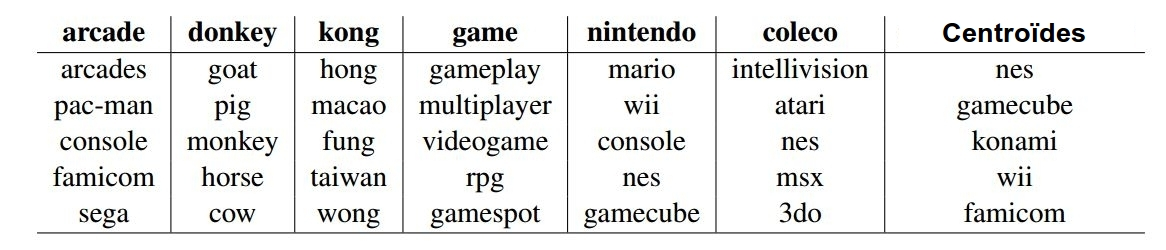
\includegraphics[height=95pt,width=420pt]{img/chapter3/centroideembed.jpg}
                \caption{Vecteurs de centroïdes}
                \label{centro-vec}
             \end{figure}

         \subsubsection{Notation des phrases}
         Dans ce processus, pour chaque phrase du document on crée un plongement pour la phrase en additionnons les plongements de mots de chaque terme dans la phrase.

        \begin{equation*}
         S\textsubscript{j} = \sum_{\substack{w\in S\textsubscript{j}}}
         E[idx(w)]
        \end{equation*}

        Afin de calculer le score finale de la phrase, on calcule la similarité de cosinus entre le plongement de la phrase S\textsubscript{j} et le plongement de la phrase centroide S\textsubscript{centroide}.
        
        \[sim\_cos(S\textsubscript{centroide},S\textsubscript{j}) = \frac {S\textsubscript{centroide} \cdot S\textsubscript{j}}{||S\textsubscript{centroide}|| \cdot ||S\textsubscript{j}||}\]
                    
                    \begin{figure}[H]
                        \centering
                        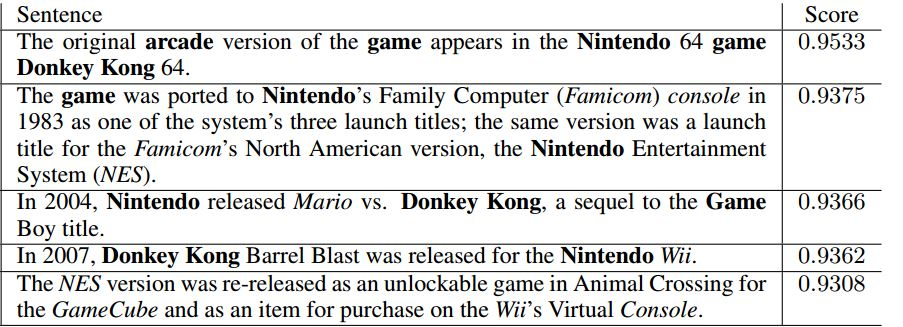
\includegraphics[height=155pt,width=400pt]{img/chapter3/scoreembed.jpg}
                        \caption{Notation des phrases}
                        \label{Notation des phrases}
                    \end{figure}

        \subsubsection{Séléction des phrases}
        Pour chaque phrase du document, on calcule la \emph{similarité de cosinus} entre elle et la phrase centroïde du document. Les phrases sont ensuite triées par ordre décroissant de leurs scores de similarité. Les phrases les mieux classées sont itérativement sélectionnés et ajoutés au résumé jusqu'à ce que la limite (taille du résumé) soit atteinte. Afin de satisfaire la propriété de redondance, au cours de chaque itération nous allons calculer la \emph{similarité de cosinus} entre la phrase a venir et chacune déjà dans le résumé.
        Il est a noter qu' un seuil a été fixé afin de rejeter toutes les phrases qui ont une similarité très élevé par rapport a une phrase afin d'éviter cette redondance.

        \begin{algorithm2e}[H]
            \SetAlgoLined
            \SetKwInOut{Input}{input}
            \SetKwInOut{Output}{output}
            \Input{phrases, scores, seuilSimilarité, seuilRésumé}
            \Output{Résumé}
            
            phrases = Tri(phrases, scores)\\
            k = 1\\
             \For{i=1 \KwTo taille(phrases)}{                
                \If{taille(Résumé) > seuilRésumé}{
                    \Return Résumé\\
                    sv = sommeVecteurs(phrases[i])\\
                    prendrePhrase = Vrai\\
                }
                \For{j=1 \KwTo k}{
                    sv2 = sommeVecteurs(Résumé[j])\\
                    sim = similarité(sv, sv2)\\
                    \If{sim > seuilSimilarité}{
                        prendrePhrase = Faux\\
                    }
                }
                \If{prendrePhrase}{
                    Résumé[k] = phrases[i]\\
                    k += 1\\      
                }
             }
             \Return{Résumé}
            \caption{Algorithme de Séléction des phrases}
        \end{algorithm2e}

        % \begin{algorithm2e}[H]
        %     \SetAlgoLined
        %     \SetKwInOut{Input}{input}
        %     \SetKwInOut{Output}{output}
        %     \Input{Résumé}
        %     \Output{RésuméTrié}
            
        %     RésuméTrié = Tri(Résumé, ordreApparitionPhrases)\\
            
        %      \Return{RésuméTrié}
        %     \caption{Algorithme de génération du résumé automatique}
        % \end{algorithm2e}

%%~~~~~~~~~~~~~~~~~~~~~~~~~~~~~~~~~~~~~~~~~~~~~~~~~~~~~~~~~~~~~~~~~~~~~~~~~~~~~~~~~~~~~~~~~%%

\section{Module de traduction}
Dans ce module, notre tâche n'était pas d'implémenter ou de concevoir un traducteur automatique, mais uniquement d'utiliser un traducteur automatique multilingue existant, et de l'intégrer dans notre architecture globale présenté dans la (figure \ref{shemaglobal}). 
Toutefois, il fallait rechercher le module de traduction le plus performant afin de traduire un article complet de la manière la plus rapide.

Afin d'intégrer un bon système de traduction automatique, nous avons explorer deux sources principales, la première était destiné a une utilisation professionnelle, de plus la version gratuite offrait une traduction pour des textes de taille limités. et la deuxième était la solution adaptée a notre système. Elle était a la fois accessible et offrait des possibilités de traduction pour des textes longs (Articles de presse, etc). 



\section{Conception de la base de données}
Le choix a été porté sur les bases de données NoSQL (\autoref{nosql}) vu la structure très dynamique des articles de presse mais aussi des profils utilisateurs.

MongoDB est une base de données orientée document écrite en C++ \cite{NOSQL3}. Les objets sont stockés en série sous la forme BSON.
Les objets n'ont pas besoin d'avoir la même structure ou les mêmes champs et les champs communs n'ont pas besoin d'avoir le même type, permettant ainsi un stockage de schéma flexible. À cet effet, nous présentons ci-dessous, sous ce format, la "collection d'articles" et la "collection des profils".

\subsection{Collection d'articles}
Les articles extraits depuis différentes sources sont tous sauvegardés sous une structure définie au préalable, prenant en considération les différences entre les formats suivies par les revu de presse. 

À cet effet nous avons choisi \emph{JSON} qui est un format léger d'échange de données. Il est facile à lire ou à écrire pour des humains\cite{json} et est pris en charge par tout les langages de programmation.

Chaque article est représenté comme suit:
\begin{itemize}
    \item \textbf{Identifiant, \textquotedbl \_id\textquotedbl: } identifiant unique d'un article de presse.
    \item \textbf{Langue, \textquotedbl language\textquotedbl:} la langue dans laquelle l'article est écrit.
    \item \textbf{Titre, \textquotedbl title\textquotedbl:} le titre de l'article.
    \item \textbf{Source, \textquotedbl source\textquotedbl:} nom de la revue de presse source.
    \item \textbf{Auteur, \textquotedbl author\textquotedbl:} on sauvegarde le nom de l'auteur.
    \item \textbf{Contenu, \textquotedbl content\textquotedbl:} contenu de l'article de presse.
    \item \textbf{Horaire, \textquotedbl publishedAt\textquotedbl:} date et heur local de publication.
    \item \textbf{Lien de l'article, \textquotedbl url\textquotedbl:} lien vers la page de l'article originale.
    \item \textbf{Lien de l'image, \textquotedbl urlToImage\textquotedbl:} lien vers l'image principale de l'article originale.
    \item \textbf{Catégorie, \textquotedbl categoryPredicted\textquotedbl:} catégorie de l'article inférée en utilisant nos modèles.
    \item \textbf{Résumé, \textquotedbl summaryGenerated\textquotedbl:} résumé automatique générée.
    \item \textbf{Traduction, \textquotedbl translatedContent\textquotedbl:} contenu de l'article de presse traduit.\\
\end{itemize}

Voici maintenant un exemple d'un document de la collection d'articles.
\begin{lstlisting}[style=code]
{
'_id': '5afc18571d41c833a8632a24', 
'language': 'en',
'title': "Smart's stellar Game 2 play draws Cavs praise", 
'source': 'espn', 
'author': 'Chris Forsberg', 
'content': 'LeBron James and Tyronn Lue explain what they think of Marcus...'
'publishedAt': '2018-05-16T05:48:55Z', 
'url': 'http://espn.go.com/nba/id/235168',
'urlToImage': 'http://espn.go.com/nba/id/235168/main.png',  
'categoryPredicted': 'sport', 
'summaryGenerated': 'The Celtics improved to 8-2 since Smart returned...', 
'translatedContent': 'sada da ada faffa fazgz eg rzgergtehk th roh...', 
},
\end{lstlisting}

\subsection{Collection de profils}
Le profile d'utilisateur regroupe très peu d'informations dans le but de protéger la vie privée. Cependant, les catégories et les sources préférées par l'utilisateur sont sauvegardées. 

Un profil utilisateur est représenté comme suit :
\begin{itemize}
    \item \textbf{Identifiant, \textquotedbl  \_id\textquotedbl : } identifiant unique.
    \item \textbf{Nom d'utilisateur, \textquotedbl  username\textquotedbl : } nom d'utilisateur unique.
    \item \textbf{Mot de passe, \textquotedbl  password\textquotedbl : } mot de passe pour l'authentification crypté.
    \item \textbf{Adreese mail, \textquotedbl  email\textquotedbl : } email de l'utilisateur.
    \item \textbf{Catégories préférées, \textquotedbl  preferences\textquotedbl : } vecteurs de catégories préférées .
    \item \textbf{Sources préférées, \textquotedbl  sources\textquotedbl : } noms des sources de revues de presse préférées. 
\end{itemize}

Ci-dessous un exemple d'un document de la collection de profils :
\begin{lstlisting}[style=code]
{
'_id': '5afc18571d41c833a8632a24', 
'username': 'yankheloufi'
'password': 'CAESEMgZsfgjSKT7GvZNAtFJaAs'
'email': 'yk@usthb.dz',
'categories': {
'entertainment': '0.63',
'world': '0.42',
'health': '0.12',
},
'sources': [
'wello-mag', 'al-jazeera-english', 'bbc-news', 
],
},
\end{lstlisting}


\section{Architecture du système \textquotedbl Feedny\textquotedbl}
Dans cette partie, nous allons présenter l'architecture globale de notre système, cette dernière est déployé sous la forme d'une architecture 3-tiers. Ci-dessous, nous présentons ce qu'est une architecture 3-tiers ainsi que son avantage avant d'expliciter un schéma de l'architecture globale.

\subsection{Présentation de l'architecture 3-tiers}
Une application Web possède souvent une architecture 3-tiers.
La couche DAO : " Data Access Object " s'occupe de l'accès aux données, le plus souvent des
données persistantes au sein d'un SGBD.

La couche métier : implémente les algorithmes " métier " de l'application. Cette couche est indé-
pendante de toute forme d'interface avec l'utilisateur.C'est généralement la couche la plus
stable de l'architecture. Elle ne change pas si on change l'interface utilisateur ou la façon
d'accéder aux données nécessaires au fonctionnement de l'application.

La couche interface utilisateur : interface (graphique souvent) qui permet à l'utilisateur de pi
loter l'application et d'en recevoir des informations.
FIGURE 3.1 – Architecture 3-tiers

\begin{figure}[H]
    \centering
    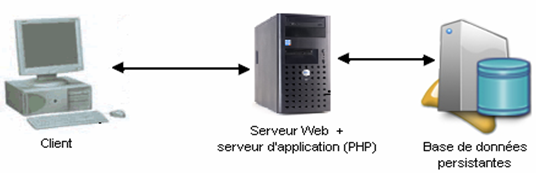
\includegraphics[height=100pt,width=400pt]{img/chapter3/tiers.png}
    \caption{Diagramme présentant les cas d'utilisations}
\end{figure}

\subsection{Avantage de l'architecture multi-tiers}
L'avantage principal d'une architecture 3-tiers (multi-tiers) est la facilité de déploiement.L'application
en elle même n'est déployée que sur la partie serveur.
Le client ne nécessite qu'une installation et une configuration minime.
En effet il suffit d'installer un navigateur web compatible avec l'application pour que le client
puisse accéder à l'application.
Cette facilité de déploiement aura pour conséquence non seulement de réduire le coût de déploie
ment mais aussi de permettre une évolution régulière du système. Cette évolution ne nécessitera
que la mise à jour de l'application sur le serveur applicatif.[4]

\subsection{Schéma global de \textquotedbl Feedny\textquotedbl}
L'architecture globale du système "Feedny" comporte quatre processus principales: Catégorisation, résumé, traduction et recommandation d'articles de presse.

Les entrées (articles de presse extraits de plusieurs sources) sont sauvegardés dans une base de données. Le processus de catégorisation commence par classifier l'article selon son contenu, ensuite un résumé est généré, l'article est traduit de l'Anglais vers l'Arabe (ou l'inverse) et enfin, il sera recommandé à un utilisateur selon son profile et ses préférences comme on peut le voir dans la figure \ref{shemaglobal}.

\begin{figure}[H]
    \centering
    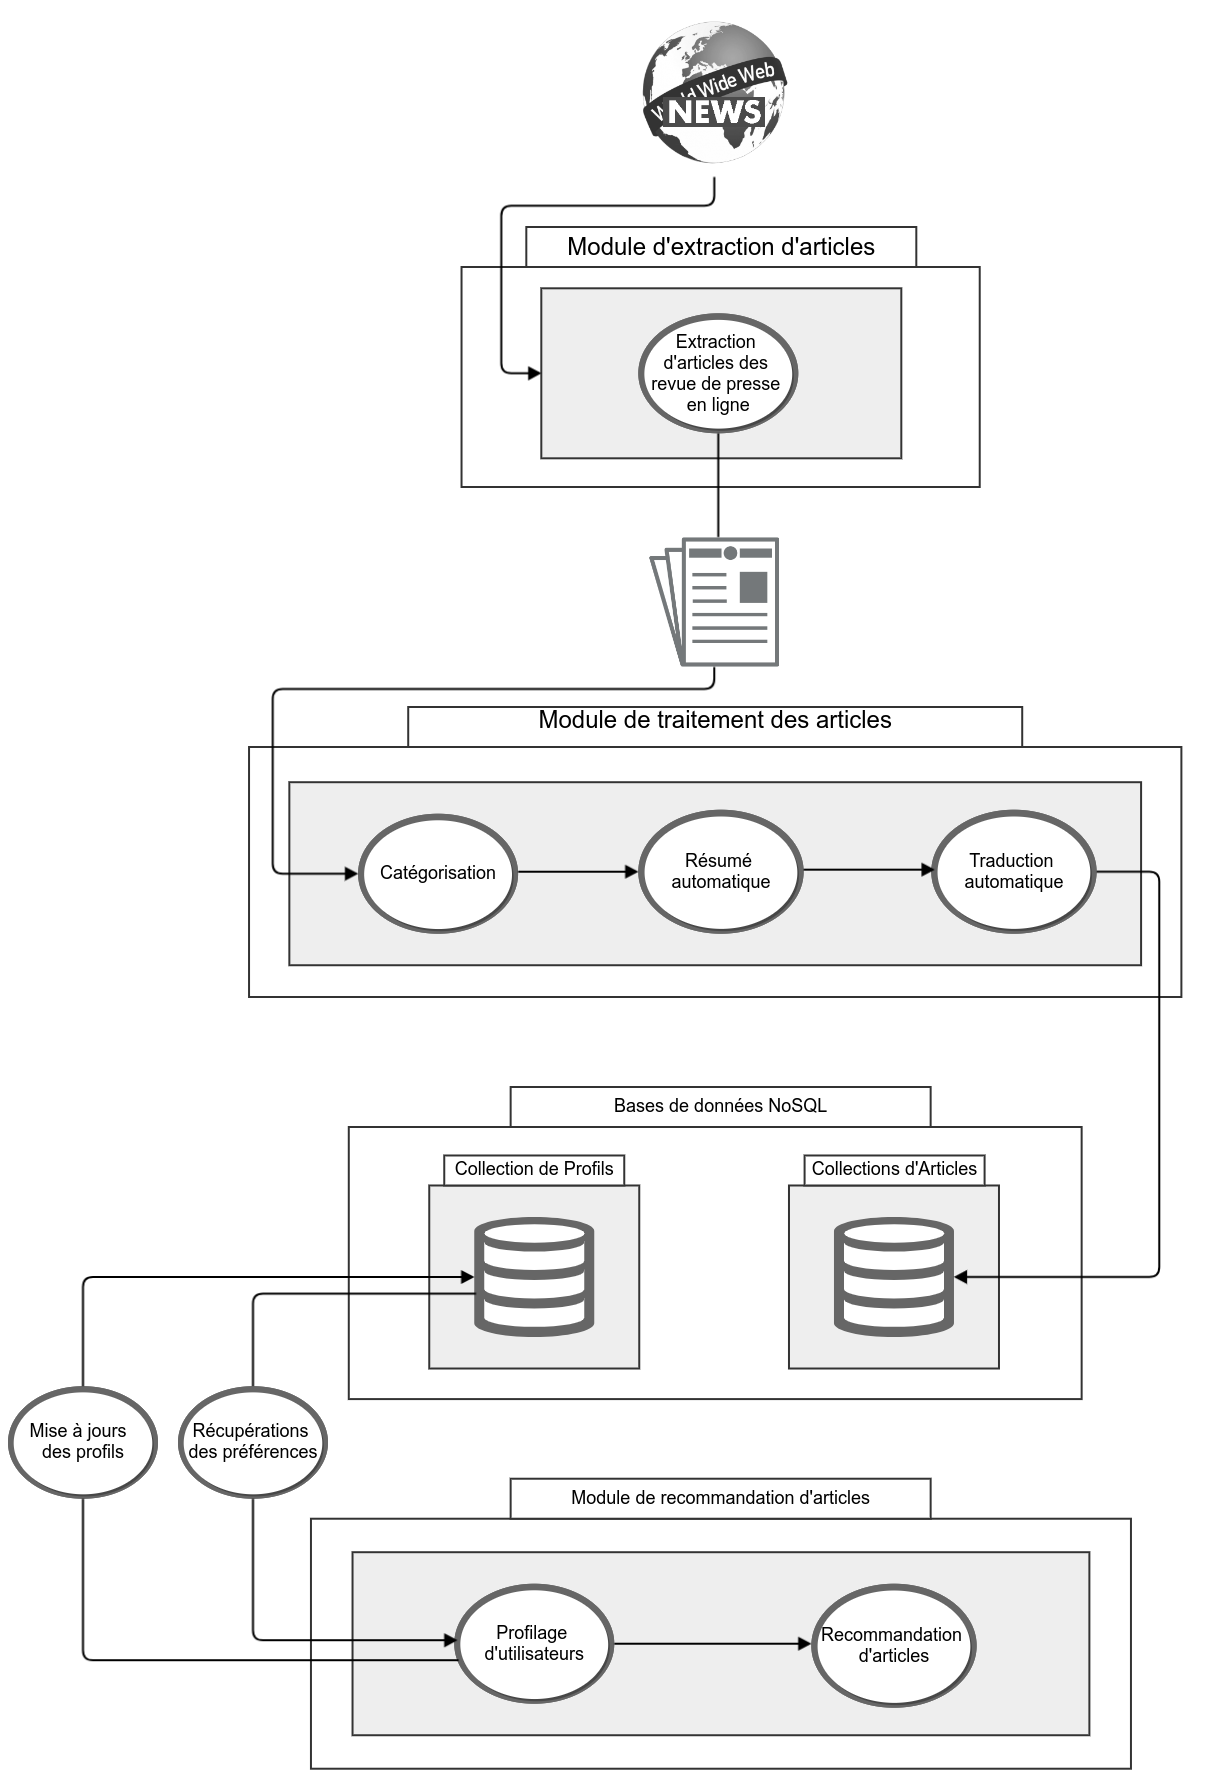
\includegraphics[height=600pt,width=450pt]{img/chapter3/global.png}
    \caption{Diagramme présentant les cas d'utilisations}
\end{figure}

%%%%%%%%%%%%%%%%%%%%%%%%%%%%%%%%%%%%%%%%%%%%%% Shéma %%%%%%%%%%%%%%%%%%%%%%%%%%%%%%%%%%%%%%%%%%%%%%%%%

\section{Schémas conceptuels de "Feedny"}
Nous allons présenter dans cette partie, la façon avec laquelle le logiciel fournit les différentes fonctionnalités. Celle-ci décrit d'une manière claire et précise, le fonctionnement du futur système en utilisant un langage de modélisation. 

Nous avons choisi la méthode UML (Unified Modeling Language), qui est une notation graphique conçue pour représenter, spécifier et construire les systèmes logiciels. UML utilise des techniques orientées objets pour la modélisation des systèmes, depuis la conception jusqu'à la maintenance, d'une manière compréhensible par l'homme et disposant de qualités formelles suffisantes pour être traduites automatiquement en code source.\cite{UML}

\subsection{Diagramme de cas d'utilisation}
"Le diagrammes de cas d'utilisation (initié par Ivar Jacobson en 1992 dans la méthode OOSE) est un type de diagramme UML qui permet de définir les besoins des acteurs dans un système quelconque en établissant les fonctionnalités attendues et en organisant les besoins. Il peut être aussi utilisés ensuite comme moyen d'organisation du développement du logiciel, notamment pour la structuration et le déroulement des tests du logiciel".\cite{UML}

\subsubsection{Diagramme de cas d'utilisation de "Feedny"}
\begin{figure}[H]
    \centering
    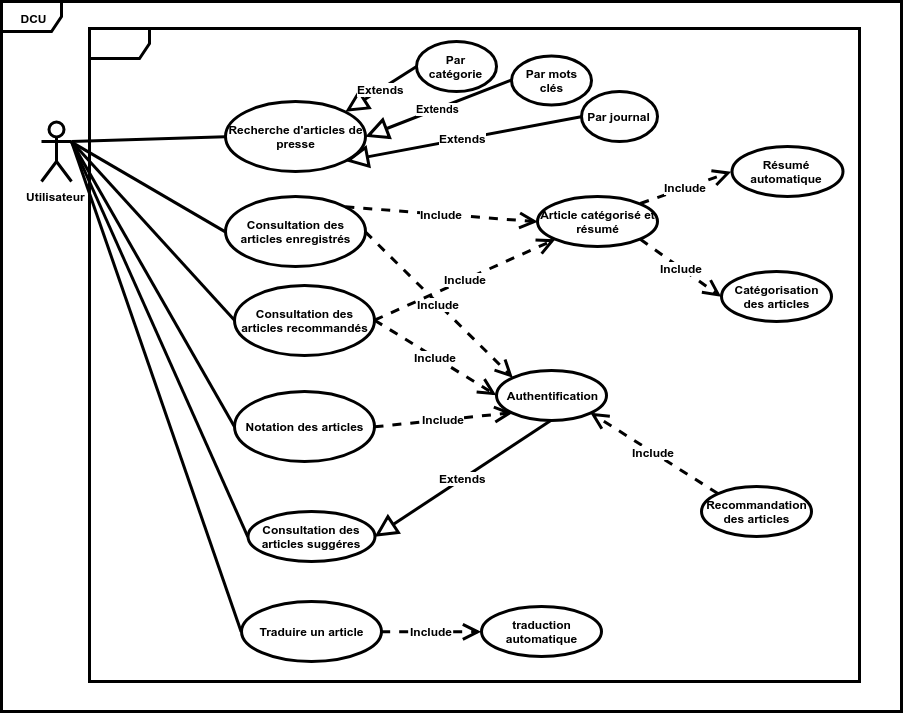
\includegraphics[height=400pt,width=350pt]{img/chapter3/diagcasdutilisation.png}
    \caption{Diagramme présentant les cas d'utilisations}
\end{figure}

\subsection{Diagramme de séquence}
Le diagramme de séquence est un diagramme UML qui fait partie des diagrammes comportementaux (dynamiques) dont L'objectif est de représenter les interactions entre les objets et les acteurs ou bien entre objets uniquement  en indiquant la chronologie des échanges. Cette représentation peut se réaliser en considérant les différents scénarios associés.\cite{UML}


\subsubsection{Diagrammes de séquence de "Feedny"}

\begin{figure}[H]
    \centering
    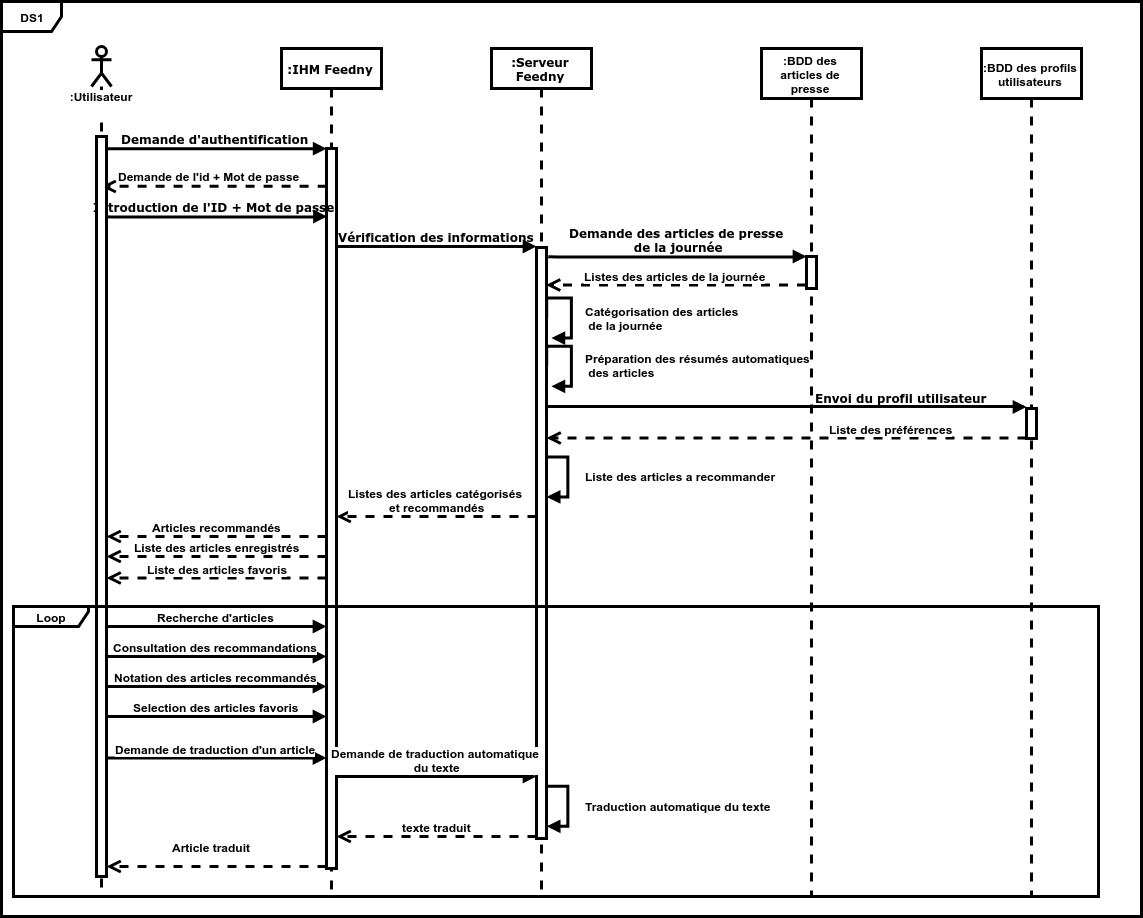
\includegraphics[height=500pt,width=425pt]{img/chapter3/diagseqperso.png}
    \caption{Diagramme de séquence dans le cas personnalisé}
\end{figure}


\begin{figure}[H]
    \centering
    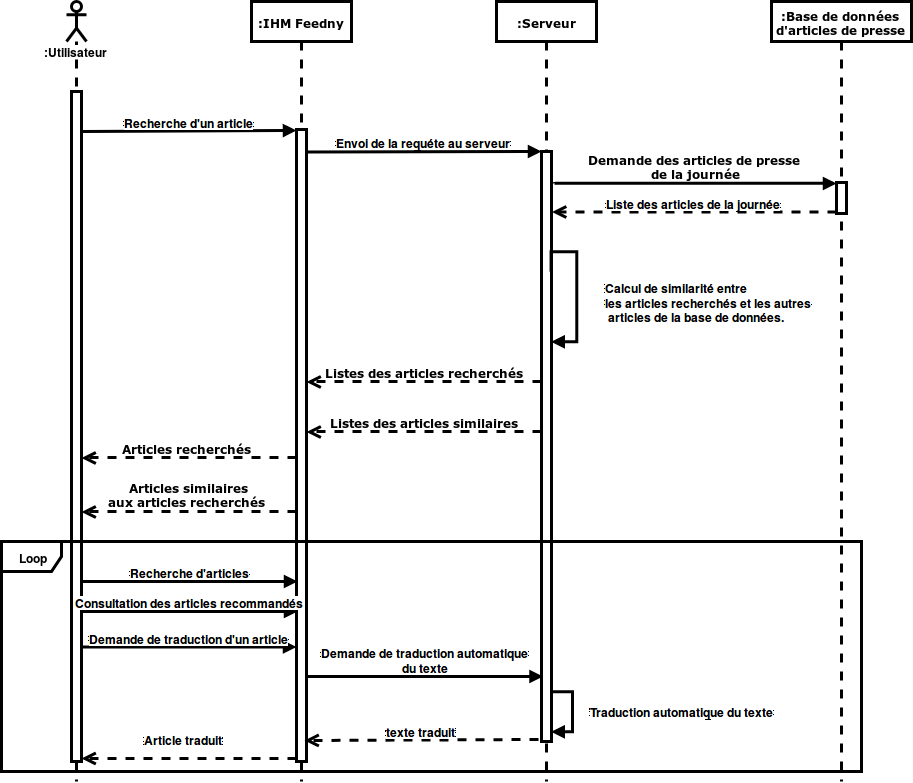
\includegraphics[height=500pt,width=425pt]{img/chapter3/diagseqnonperso.png}
    \caption{Diagramme de séquence dans le cas non personnalisé}
\end{figure}

\section{Mesures d'évaluation du système}
    \subsection{Métriques d'évaluations du module de résumé automatique}
        \subsubsection{Métrique d'évaluation : ROUGE\label{metrique-eval}}
        ROUGE est l'acronyme de "Recall-Oriented Understudy for Gisting Evaluation". Il s'agit essentiellement d'un ensemble de métriques permettant d'évaluer le résumé automatique de textes ainsi que la traduction automatique. Il fonctionne en comparant un résumé produit automatiquement ou une traduction à un ensemble de résumés de référence (généralement produits par des humains). \cite{rouge0}

        \subsubsection{Types des métriques de ROUGE\label{type-rouge}}
        \begin{itemize}
            \item{ROUGE-1, 2, 3 et 4 : font référence au chevauchement des uni-grammes, bi-grammes, tri-grammes et quadri-grammes, respectivement, entre le système et les résumés de référence \cite{rouge1}.}\\
            \item{ROUGE-L, W : basés sur la plus longue sous-séquence commune (LCS) \cite{rouge2}.}\\
            \item{ROUGE-S : basé sur les cooccurrences des paires de mots dans l'ordre des phrases \cite{rouge2}.}\\
            \item{ROUGE-SU : en plus des paires de mots, il utilise aussi la cooccurrence du mot unique toujours dans l'ordre des phrases.}
        \end{itemize}

        Les métriques citées dans la \autoref{type-rouge}, utilisent comme mesures le rappel, la précision et la f-mesure :  
        \begin{itemize}
            
            \item {Le rappel dans le cas de ROUGE, donne une information sur le nombre de mots du résumé de référence ont été capturés par le résumé de notre généré par le système.\\ 
                Exemple: si le rappel est égal a 40\%, cela signifie que 40\% des n-grammes du résumé de référence sont également présents dans le résumé généré par le système.}\\
            \item {La précision quant à elle, mesure la partie du résumé du système qui est pertinente ou nécessaire.\\ 
                Exemple : si la précision est égale a 40\%, cela signifie que 40\% des n-grammes du résumé généré par le système sont également présents dans le résumé de référence.}
            \item {La f-mesure dépend de la précision et le rappel et est calculé comme suit :\\
                                \[ F-mesure = \frac{2 * (Precision * Rappel)} {(Precision + Rappel)} \]}

        \end{itemize}

    \subsection{Métriques d'évaluations du module de catégorisation}
    \begin{itemize}
        \item{\textbf{Accuracy :} }c'est une mesure qui évalue l'efficacité globale de l'algorithme par rapport au données de test.
        \[ Accuracy = \frac{tp+tn} {tp+fp+tn+fn} \]
        \item{\textbf{Précision :} }elle évalue le pouvoir prédictif du modèle en mesurant la capacité du modèle à prédire que des classes correctes.
        \[ Precision = \frac{tp} {tp+fp} \]
        \item{\textbf{Rappel :} }la capacité d'un modèle à prédire toutes les classes correctes de l'ensemble de test.
        \[ Rappel = \frac{tp} {tp+fn} \]
        \item{\textbf{F-mesure :} }une mesure composite qui profite aux algorithmes avec une sensibilité plus élevée et des algorithmes de défis avec spécificité plus élevée.!!!
        \[ F-mesure = \frac{2 * (Precision * Rappel)} {(Precision + Rappel)} \]
    \end{itemize}
    Avec :
    \begin{itemize}
        \item{\textbf{TP }True Positive (vrais positifs) :} nombre d'individus bien prédits dans la classe à juste titre.
        \item{\textbf{FP }False Positive (faux positifs) :} nombre d'individus prédits d'une classe alors qu'ils ne devraient pas en faire parti.
        \item{\textbf{FN }False Negative (faux négatifs) :} nombre d'individus prédits comme étant de la classe alors qu'il ne le sont pas en vrai.
        \item{\textbf{TN }True Negative (vrais négatifs) :} nombre d'individus prédits comme n'étant pas dans la classe à juste titre.
    \end{itemize}

\chapter{Implémentation et résultats}    
%!TEX program=luatex

\newpage
\section{Introduction}
Après avoir finalisé l'étape de conception, nous consacrons ce chapitre à la réalisation. Les différentes problématiques ont étaient profondément analysées, ce qui nous a permit d'entreprendre le développement des modules, ayant comme objectif d'aboutir à un produit final exploitable par les utilisateurs.

Nous allons d'abord présenter l'environnement de travail ainsi que les outils et les logiciels utilisés, nous décrivons également en détails les étapes de réalisation de chaque module, et nous clôturons avec l'évaluation et les résultats de notre système ainsi que l'application mobile réalisée.
\section{Environnement et outils de travail}
    \subsection{Matériels}
    Le matériel utilisé consiste en 2 ordinateurs personnels ainsi qu'un serveur (Cloud) dédié aux traitements gourmands en terme de ressource et en temps d'exécution.
    \begin{enumerate}
        \item{\textbf{Poste de travail 1}}
        \begin{table}[h!]
            \begin{center}
                \begin{tabular}{|C{5cm}|C{8cm}|}
                    \hline
                    \textbf{Système d'exploitation} &  GNU/Linux Ubuntu 16.04 xenial 64bits \\
                    \textbf{RAM} &  4 Go \\
                    \textbf{Processeur} & Intel Core i3-3110M CPU @ 2.4GHz \\
                    \hline
                \end{tabular}
            \end{center}
        \caption{Caractéristiques du poste de travail 1}
        \end{table}

        \item{\textbf{Poste de travail 2}}
        \begin{table}[h!]
            \begin{center}
                \begin{tabular}{|C{5cm}|C{8cm}|}
                    \hline
                    \textbf{Système d'exploitation} &  Windows 8.1 64bits \\
                    \textbf{RAM} &  12 Go \\
                    \textbf{Processeur} & Intel Core i7-5500 CPU @ 2.40 GHZ \\
                    \hline
                \end{tabular}
            \end{center}
        \caption{Caractéristiques du poste de travail 2}
        \end{table}

        \item{\textbf{Serveur (Cloud Virtual Machine)}}
        \begin{table}[h!]
            \begin{center}
                \begin{tabular}{|C{5cm}|C{8cm}|}
                    \hline
                    \textbf{Système d'exploitation} &  GNU/Linux Ubuntu Data Science 64bits \\
                    \textbf{RAM} &  32 Go \\
                    \textbf{Processeur} & Intel Xeon CPU E5-2673 v4 @ 2.295GHz \\
                    \hline
                \end{tabular}
            \end{center}
        \caption{Caractéristiques de la machine virtuelle}
        \end{table}
    \end{enumerate}   

    \subsection{Langages de programmation et logiciels}
    Nous avons utilisé au cours de la réalisation de notre système, plusieurs langages de programmation et logiciels. Ci-après une brève présentation de ces derniers :
        \subsubsection{Langages de programmation}
            \begin{figure}[H]
                    \centering
                    
\includegraphics[height=60pt,width=200pt]{img/chapter4/tools/language.png}
                    \caption{Logos des langages de programmations utilisés}
                    \label{}
            \end{figure}
            \begin{enumerate}[leftmargin=*]
                \item{\textbf{Python : }}
                Python est un langage de programmation de haut niveau. Il supporte la programmation impérative structurée, fonctionnelle et orientée objet. Il est doté d'un typage dynamique fort, d'une gestion automatique de la mémoire. Plusieurs bibliothèques sont fournies afin de faciliter les développements \cite{python}.\\

                \item{\textbf{JavaScript : }}
                Langage de programmation de scripts principalement employé dans les pages web interactives mais aussi pour les serveurs avec l'utilisation (par exemple) de \emph{Node.js}. Il supporte le paradigme objet, impératif et fonctionnel. JavaScript est le langage possédant le plus large écosystème grâce à son gestionnaire de dépendances \emph{npm}, avec environs 500 000 paquets en août 2017 \cite{javascript}.\\

                \item{\textbf{React-Native : }}
                Framework mobile hybride Open source développé par Facebook depuis début 2015. Il continue d'évoluer avec le soutient de nombreux contributeurs. Le but de React Native est de pouvoir réutiliser le maximum de code entre les différentes plate-formes (iOS et Android). Il offre un gain de temps considérable par rapport à du développement spécifique, tout en étant aussi performant \cite{reactnative}.
            \end{enumerate}

        \subsubsection{Librairies et bibliothèques}
            \begin{figure}[h]
                    \centering
                    
\includegraphics[height=150pt,width=320pt]{img/chapter4/tools/tools.png}
                    \caption{Logos de quelques librairies utilisées}
                    \label{}
            \end{figure}
            \begin{enumerate}[leftmargin=*]
                \item{\textbf{NLTK : }}
                "Natural Language Toolkit" est une librairie Python destinée au TALN. Elle fournit une suite de bibliothèques de traitement de texte pour la classification, tokenization, stemming, étiquetage, analyse et raisonnement sémantique, etc. \cite{nltk}.\\

                \item{\textbf{Scikit-Learn : }\label{scikit-learn}}
                Bibliothèque libre et Open source implémenté avec Python, dédiée à l'apprentissage automatique. Elle est conçue pour s'harmoniser avec d'autres bibliothèques Python (ou autres), notamment NumPy, SciPy, etc. \cite{scikit}.\\

                \item{\textbf{Numpy : }}
                "Numerical Python" fournit une interface pour stocker et effectuer des opérations sur les données. D'une certaine manière, les tableaux Numpy sont comme les listes en Python, mais Numpy permet de rendre les opérations beaucoup plus efficaces, surtout sur les tableaux de grande taille qui sont au cœur de l'écosystème de la Data Science \cite{numpy}.\\
                
                \item{\textbf{Gensim : }}
                Librairie Python gratuite conçue pour extraire automatiquement des sujets sémantiques à partir de documents. Les algorithmes de Gensim, tels que l'analyse sémantique latente, permettent de découvrir la structure sémantique des documents en examinant les schémas statistiques de cooccurrence des mots au sein d'un corpus de documents \cite{gensim}.\\

                \item{\textbf{Pandas : }}
                Fournit deux structures de données fondamentales, la "Série" et le "DataFrame". On peut voir ces structures comme une généralisation des tableaux et des matrices de Numpy. La différence entre les structures de Pandas et celles de Numpy c'est la définition explicites par l'utilisateur des indices et des index sur les objets (matrices) .\cite{pandas}\\

                \item{\textbf{Pickle : }}
                Module Python utilisé pour sérialiser et désérialiser les structures d'objets Python. La sérialisation (ou «pickling») fait référence au processus de conversion d'un objet en mémoire en un flux d'octets pouvant être stocké sur disque ou envoyé sur un réseau. Plus tard, ce flux de caractères peut être récupéré et désérialisé (ou «unpickling») en retour vers un objet Python \cite{pickle}.\\

                \item{\textbf{Matplotlib : }}
                "Mathematic Plot library" est une bibliothèque de traçage Python 2D qui produit des figures de qualité de publication dans une variété de formats papier et d'environnements interactifs entre plates-formes. Matplotlib peut être utilisé dans les scripts Python, les Shells Python et IPython, les notebook Jupyter, etc. \cite{matplotlib}.\\

                \item{\textbf{Newspaper : }}
                Librairie Python accessible gratuitement qui permet d'extraire le contenu, l'image, les auteurs et la date de publication d'un article de presse en utilisant le protocole HTTP.\\

                \item{\textbf{Newsapi : }}
                Web API qui permet d'obtenir des articles de presse de dernière minute et de rechercher des articles de plus de 30 000 sources et blogs. Elle fournit également la possibilité de sélectionner les sources, les pays, les catégories, etc.\\

                \item{\textbf{FeedParser : }}
                "Universal Feed Parser" est une librairie Python pour le téléchargement et l'analyse des flux syndiqués connu sous l'appellation \emph{flux RSS}. Cette librairie se distingue par sa facilité d'utilisation \cite{feedparser}.\\

                \item{\textbf{TextBlob : }}
                Toolbox Python pour le traitement des données textuelles. Elle fournit une API simple permettant de plonger dans des tâches courantes de TALN, telles que l'étiquetage, l'extraction de syntagmes nominaux, l'analyse des sentiments, la classification, la traduction automatique, etc. \cite{textblob}\\

                \item{\textbf{Farasa : }}
                L'équivalent arabe de "perspicacité", Farasa est une Toolbox de traitement de la langue naturel arabe développé au sein de l'institut \emph{Qatar Computing Research Institute}. Elle est composée de plusieurs modules : segmentation, étiquetage, etc. Farasa surpasse ou égalise les deux fameuses Toolbox pour l'arabe Stanford NLP et MADAMIRA \cite{farasa}.\\

                \item{\textbf{PyRouge : }}
                Interface Python pour le fameux module d'évaluation des résumés automatique ROUGE. Elle facilite l'utilisation de ROUGE avec la conversion des fichiers qui contiennent les résumés en un format interprétable par ROUGE et génère automatiquement les fichiers de configuration ROUGE \cite{pyrouge}.\\

                \item{\textbf{PyMongo}}
                Module de gestion du SGBD MongoDB sous le langage Python, il fournit une variété de commandes très intéressantes qui permettent de faciliter la manipulation d'une base de donnée NoSql \cite{pymongo}.\\
            \end{enumerate}

        \subsubsection{Formats de données}
            \begin{enumerate}[leftmargin=*]
                \item{\textbf{XML : }}
                "eXtensible Markup Language" est un langage informatique de balisage générique. Ces balises permettent de structurer de manière hiérarchisée et organisée les données d'un document.\\

                \item{\textbf{JSON : }}
                "JavaScript Object Notation" est un format adapté aux types de données du langage JavaScript. Au cours des dernières années, JSON est devenu l'un des premiers format d'échange et de stockage de données notamment pour le développement web \cite{jsonimpl}.\\
                
                \item{\textbf{CSV : }}
                "Comma-separated values" est un format informatique représentant des données tabulaires sous forme de valeurs séparées par des virgules. Le format de fichier CSV est utilisable par les applications de tableur KSpread, OpenOffice Calc, Microsoft Excel, etc. De nombreuses autres applications prennent en charge CSV pour importer ou exporter des données.\cite{csv}
            \end{enumerate}

        \subsubsection{Logiciels et éditeurs de textes}
            \begin{figure}[H]
                    \centering
                    
\includegraphics[height=80pt,width=250pt]{img/chapter4/tools/software.png}
                    \caption{Logos des logiciels utilisés}
                    \label{}
            \end{figure}
            \begin{enumerate}[leftmargin=*]
                \item{\textbf{PyCharm Community Edition : }}
                PyCharm est un éditeur de code pour le développement sous Python, il fournit la complétion de code intelligente, des inspections, la mise en évidence d'erreurs à la volée et des correctifs rapides, ainsi que des corrections de code automatisés et de riches fonctionnalités de navigation.\cite{pycharm} Le version \emph{Community Edition} que nous avons utilisé est gratuite et en libre accès.\\

                \item{\textbf{WebStorm : }}
                WebStorm est un éditeur de code pour le développement sous Javascript, il apporte une aide énorme au développeurs web et mobile. Il supporte tout les langages compilés au JavaScript, Node.js, HTML et CSS \cite{webstorm}. Nous avons pu obtenir une licence étudiant d'une année.\\

                \item{\textbf{Sublime Text : }}
                Éditeur de texte générique codé en C++ et Python, disponible sur Linux, Mac et Windows. Depuis la version 2.0, sortie le 26 juin 2012, l'éditeur prend en charge 44 langages de programmation majeurs, tandis que des plugins sont souvent disponibles pour les langages plus rares \cite{sublime}. Nous avons utilisé la version d’essai qui est en libre accès sur internet.\\

                \item{\textbf{Git : }}
                Système de gestion de versions décentralisé. C'est un logiciel libre créé par \emph{Linus Torvalds}, auteur du noyau Linux, et distribué selon les termes de la licence publique générale (GPL). En 2016, il s’agit du logiciel de gestion de versions le plus populaire qui est utilisé par plus de douze millions de personnes \cite{git}.
            \end{enumerate}



\section{Recommandation}
\subsection{Approche probabilité de sélection}  
Afin d'implémenter cette approche et tenter de générer une collection de profils utilisateurs, nous avons essayer d'utiliser des datasets destinés au articles de presse. Ci-dessous, une description des datasets utilisés.

\subsubsection{SmartMedia Adressa News Dataset}
Le dataset Adressa est un ensemble de données d'actualité comprenant des articles de presse (en norvégien) en lien avec des utilisateurs anonymes. Cet ensemble de données est publié avec la collaboration de l'Université norvégienne des sciences et technologies (NTNU) et Adressavisen (journal local à Trondheim, Norvège) dans le cadre du projet RecTech sur la technologie de recommandation.\cite{refnorvege}

\subsubsection{Structure du dataset}


Exemple :


\subsubsection{Statistiques sur le dataset}


\subsubsection{Inconvénients de l'utilisation de \textquotedbl SmartMedia Adressa News Dataset\textquotedbl}

Le dataset décrit dans cette partie traite les articles de presse en langage nowégien, c'est a dire que les catégories des articles sont en norwégien et le contenu des articles aussi. Ce qui nous a amené a abandonné ce dataset.
  
\subsubsection{Le dataset \textquotedbl YOW \textquotedbl}
Afin de concevoir une base de données de profils utilisateurs, nous avons solliciter \emph{Google News}, \emph{Bing News} et \emph{Yahoo Webscope} mais sans aucune réponse de la part de ces entreprises. 

Mais au final, nous avons pu obtenir le dataset \emph{YOW} qui est le seul dataset d'interactions des profils avec des articles de presse. 

\emph{Yow} été collecté à l'Université \emph{Carnegie Mellon} pour le \emph{Yow-now} le système de filtrage des articles de presse \cite{carnegieYOW}.

Le dataset YOW est composé de plusieurs attribut, des informations sur les interactions de 22 utilisateurs avec des articles de presse de différentes catégories. Les instances du dataset sont très bien adapté au filtrage collaboratif. Comme il n'y a pas d'information sur le contenu des articles de presse, le filtrage basé sur le contenu n'est pas possible. 

\subsubsection{Structure du dataset}
Chaque instance du dataset YOW est composé de 23 attribut propre à l'utilisateur et à l'article de presse. Ci-après les attributs les plus importants pour notre système de recommandations :  
\begin{lstlisting}[style=code] 
{
'user_id': '19', 
'document_id': '27010084'
'timestamp': '2004-04-23T15:38:25Z'
'timeonpage': '63s', #temps de lecture
'classes': [
'space', 'international', 'iraq', 
],
...
},
\end{lstlisting}

\subsubsection{Statistiques sur le dataset}
Yow-now est un système de filtrage d'informations qui recommande des articles de presse aux utilisateurs à partir de divers flux RSS. Les données sont recueillies par une étude d'un mois qui comprend environ 25 personnes et plus de 7000 entrées de commentaires de tous les utilisateurs. Au total 383 articles évalués par chaque utilisateur. 

Le dataset comporte également des évaluations implicite et explicite sur les recommandations. Le profilage explicite est sous forme de note de 1 à 5, quant à l'implicite est établi selon les interactions de l'utilisateur (souris, clavier et activités de défilement).


\subsubsection{Pré-traitement des données}
Chaque instance du dataset \emph{YOW} est une interaction de l'utilisateur U avec un article A.

L'interaction peut avoir plusieurs valeurs pour l'attribut \emph{Classe} (catégorie dans notre cas). "Classe" peut prendre des noms de catégories et des mots-clés de l'article, par exemple :
\begin{itemize}
    \item Noms de catégories : world, science, entertainment, space, business, food, etc.
    \item Mots-clés :Iraq, Amazon, Malaysia, Oil, Japan, etc.\\ 
\end{itemize}
Pour adapter ces données à notre modèle de catégorisation d'article nous avons effectué des pré-traitement sur chaque instance du dataset. Nous avons annoter le dataset manuellement dans le but de convertir les noms de catégories et les mots-clés en catégories présente dans notre système (7 pour l'Anglais et 6 pour l'Arabe), par exemple :
\begin{itemize}
    \item Avant : nuclear weapons, international, middle east, business, John Kerry, accident, tradegy, space, science.
    \item Après : 
    \begin{itemize}
        \item {nuclear weapons, international, middle east} : World
        \item {John Kerry} : US
        \item {space, science} : Science \& Technology
        \item {accident, tradegy} : Society
        \item {business} : Business\\
    \end{itemize}    
\end{itemize}
De plus, le dataset a été classé dans l'ordre croissant de l'attribut "Timestamp", la date et l'horaire de l'interaction, dans le but de récupérer l'historique et le changement des centres d’intérêts de chaque utilisateur. 

À chaque nouvelle interaction le vecteur de probabilité de sélection des catégories d'articles se mets à jour en fonction de l'article visité. 

La mise à jour consiste en l'augmentation de la probabilité de sélection de la catégorie de l'article choisie et la diminution des autres catégories (s'il y-en a). 

L'exemple suivant montre le processus de mise à jour :
\begin{itemize}[label={}]
    \item $P = {'news': 0.0581,'sport': 0.717, 'sci\_tech': 0.149}$\\
\end{itemize}

L'utilisateur X a cliqué et lu un article de la catégorie \emph{Sport}, le vecteur de probabilité de sélection va se mettre à jour en fonction de cette dernière interaction (détails dans \ref{proba-select}).
\begin{itemize}[label={}]
    \item $P[sport] = (1-{\alpha}) * {P[sport]} + {\alpha}$
    \item $P[sport] = (1-{0.1}) * {P[sport]} + {0.1}$
    \item $P[sport] = (1-{0.1}) * {0.717} + {0.1}$
    \item $P[sport] = 0.745$
\end{itemize}

Quant aux autres catégories du vecteurs de sélection :
\begin{itemize}[label={}]
    \item $P[news] = (1-{\alpha}) * {P[news]} $
    \item $P[news] = (1-{0.1}) * {P[news]} $
    \item $P[news] = (1-{0.1}) * {0.0581} $
    \item $P[news] = 0.0523$
    \item 
    \item $P[sci\_tech] = (1-{\alpha}) * {P[sci\_tech]} $
    \item $P[sci\_tech] = (1-{0.1}) * {P[sci\_tech]} $
    \item $P[sci\_tech] = (1-{0.1}) * {0.1499} $
    \item $P[sci\_tech] = 0.135$
\end{itemize}
Après cette interaction, le vecteur de probabilité de sélection devient :
\begin{itemize}[label={}]
    \item $P = {'news': 0.0523, 'sport': 0.745, 'sci_tech': 0.135}$\\
\end{itemize}
Pour un nouvel utilisateur, le même traitement est appliqué, le vecteur de probabilité de sélection se remplie petit à petit en fonction des interaction qui vont être mise à jour de la même façon.

\subsubsection{Utilisateur non identifier}
Dans le cas où l'utilisateur n'est pas connecté, donc il n’y a pas de vecteur de probabilité de sélection, la recommandation est basée sur la similarité entre articles.

Si l'utilisateur U a lu l'article A1, les articles A2, A3, ..., An similaires à A1, seront recommandés. La similarité entre article est calculé à partir du contenu, le texte sera convertit en TF-IDF et les articles les plus proches en calculant la similarité du Cosinus seront considérés comme article qui parle du même sujet ou de la même catégorie.

\begin{itemize}[leftmargin=*]
    \item Exemple :\\ 
    A1 = "Real Madrid 3-1 Liverpool: Jurgen Klopp says Reds wanted everything and got minus something"\\
    Articles similaires à A1 = \{\\
    'Gareth Bale on his Champions League final goal for Real Madrid': 0.26435,\\
    'Real Madrid 3-1 Liverpool: ‘Flawed Karius pays for lack of focus’': 0.21839,\\
    'Columbus Crew: Two US cities fight over one football team': 0.073586
    \}
\end{itemize} 

\section{Catégorisation}
    Le deuxième module sur lequel nous avons travailler, c'est la catégorisation d'articles de presse. Nous avons expérimenter plusieurs techniques proposées dans la littérature. Nous présentons ci-après chaque approche, ses résultats, ses points forts et ses faiblesses.
    \subsection{Approches expérimentées\label{approches}}
        Toutes les approches utilisées sont basées sur l'apprentissage automatique, supervisé et non supervisé. 
        \subsubsection{Basées sur l'Apprentissage Non Supervisé}
            \begin{itemize}
                \item{LDA (Latent Dirichlet Allocation) : }
            \end{itemize}

        \subsubsection{Basées sur l'Apprentissage Supervisé}
            \begin{table}[H]
                    \begin{center}
                        \begin{tabular}{|c|c|c|c|c}
                            \hline
                            \textbf{Modèle} & \textbf{Précision} & \textbf{Rappel} & \textbf{F-mesure} \\
                            \hline
                            Naïve de Bayes & 0.89 & 0.87 & 0.88 \\
                            Arbre de décision & 0.82 & 0.84 & 0.83 \\
                            \textbf{Descente de Gradient Stochastique} & \textbf{0.94} & \textbf{0.94} & \textbf{0.94} \\
                            SVM & 0.91 & 0.89 & 0.90 \\
                            \hline
                        \end{tabular}
                    \end{center}
                    \caption{Résultats comparatifs des modèles de catégorisation pour l'arabe}
                    \label{modele-categ}
                \end{table}
                
    \subsection{Corpus et dataset}
        Comme tout problème de classification, la catégorisation d'articles de presse nécessite de très grandes masses de données. C'est pour cela que nous avons consacrer une bonne période du projet à la récolte des corpus et la préparation des datasets.     
        \subsubsection{Quelques chiffres et statistique}
            \begin{itemize}
                \item{\textbf{Anglais : }}
                 Le dataset baptisé "News" a été récolté par le Laboratoire Informatique de \emph{l'Université de Pise} \cite{pise}, il regroupes des articles de 3 sources différentes : \emph{The New York Times}, \emph{Reuters} et \emph{USA Today}. le Tableau \ref{news-categ} présente en détails le nombre d'articles de chaque catégorie.
                \begin{table}[H]
                    \begin{center}
                        \begin{tabular}{|C{5cm}|C{5cm}|}
                            \hline
                            \textbf{Catégorie} &  \textbf{Nombre d'articles} \\
                            \hline
                            Business & 5366 \\                            
                            Entertainment & 3286 \\
                            Health & 1851 \\
                            Science \& Technology & 2872 \\
                            Sport & 8189 \\
                            US & 4783 \\
                            World & 6255 \\
                            \textbf{Totale} &  \textbf{32602} \\
                            \hline
                        \end{tabular}
                    \end{center}
                    \caption{Nombres d'articles de chaque catégorie du corpus "News"}
                    \label{news-categ}
                \end{table}
                \item{\textbf{Arabe : }}
                Le corpus TALAA\footnote{Traitement Automatique du Langage et Apprentissage Automatique, l'équipe de recherche du Laboratoire de Recherche en Intelligence Artificielle du département informatique de l'USTHB} pour la catégorisation d'articles de presse est une grande collection d'articles publiés entre 2010 et 2014 dans différentes revue de presse Arabe sur internet. Il contient plus de 14 millions de mots de 582000 types différents. Le corpus contient 8 catégories, mais nous avons choisi de travailler sur 6 catégories plus générales comme on peut le constater dans le tableau suivant \ref{talaa-categ} \cite{talaa}. 
                \begin{table}[H]
                    \begin{center}
                        \begin{tabular}{|c|c|}
                            \hline
                            \textbf{Catégorie} &  \textbf{Nombre d'articles} \\
                            \hline
                            \begin{arab}الجزائر\end{arab} & 6603 \\
                            \begin{arab}الثقافة\end{arab} & 3311 \\
                            \begin{arab}الدين\end{arab} & 2568 \\
                            \begin{arab}المجتمع\end{arab} & 7714 \\
                            \begin{arab}الرياضة\end{arab} & 8104 \\
                            \begin{arab}العالم\end{arab} & 4380 \\
                            \textbf{Totale} & \textbf{32680} \\
                            \hline
                        \end{tabular}
                    \end{center}
                    \caption{Nombres d'articles des 6 catégories choisies du corpus "TALAA"}
                    \label{talaa-categ}
                \end{table}
            \end{itemize}
        \subsubsection{Pré-traitement et structure des datasets}
            Les deux corpus utilisés dans les deux langues étaient sous le format brute, ce qui nécessitaient une restructuration et un pré-traitement afin de permettre leur exploitation.  

            Plusieurs opérations de pré-traitements ont été effectuées. Ci-après les étapes suivies :
            \begin{enumerate}
                \item{\textbf{Segmentation (Tokenization) et suppression des mots vides :} } Pour l'Anglais nous avons utiliser le Tokenizer natif de NLTK, et FARASA Toolbox pour la langue Arabe.\\  
                
                \item{\textbf{Racinisation (Stemming) :} } 
                La librairie Snowball Stemmer de NLTK a été utilisé pour l'Anglais, quant à l'Arabe c'est toujours la Toolbox FARASA.\\

                \item{\textbf{N-grammes :} }
                 L'algorithme natif de NLTK a été utilisé pour les deux langues (Anglais et Arabe).\\ 
                
                \item{\textbf{Extraction des caractéristiques :} }
                Les librairies Countvectorizer et tfidfvectorizer de scikit-learn ont été utilisés dans l'éxtraction des caractéristiques pour l'anglais et l'arabe.\\
            \end{enumerate}

            
    \subsection{Modèles finaux}
        Après expérimentation des techniques citées dans \ref{approches}, voici les modèles finaux de la catégorisation d'articles de presse implémentés en Python en utilisant la librairie Scikit-learn \ref{scikit-learn} :
        \begin{itemize}
            \item{\textbf{Anglais :} }le modèle le plus performant est obtenu en utilisant l'algorithme SVM avec 80\% de données pour l'apprentissage et le 20\% restant pour les tests sur un total de 32602 articles de 7 catégories différentes.\\

            \item{\textbf{Arabe :} }l'algorithme de la Descente de Gradient Stochastique nous a donné les meilleurs résultats en utilisant 32680 articles, avec 75\% de données pour l'apprentissage et le reste pour les tests. 
        \end{itemize}
    \subsection{Résultats et évaluation}
        \subsubsection{Résultats}
        \begin{itemize}
            \item{\textbf{Anglais :}}
            \begin{itemize}
                \item{Accuracy : 0.987}
                \item{Précision : 0.988}
                \item{Rappel : 0.982}
                \item{F-mesure : 0.985}
            \end{itemize}
            \begin{table}[H]
                    \begin{center}
                        \begin{tabular}{|c|C{2cm}|C{2cm}|C{2cm}|C{2cm}|}
                            \hline
                            \textbf{Catégorie} &  \textbf{Précision} &  \textbf{Rappel} &  \textbf{F-mesure} &  \textbf{Support} \\
                            \hline
                            Business & 0.98 & 0.96 & 0.97 & 1046 \\
                            Entertainment & 0.99 & 0.99 & 0.99 & 651 \\
                            Health & 0.97 & 1.00 & 0.99 & 388 \\
                            Science \& Technology & 0.94 & 1.00 & 0.97 & 546 \\
                            Sport & 1.00 & 1.00 & 1.00 & 1635 \\
                            US & 0.99 & 0.98 & 0.99 & 993 \\
                            World & 1.00 & 0.99 & 0.99 & 1262 \\                          
                            \textbf{Moyenne/Totale} & \textbf{0.99} & \textbf{0.98} & \textbf{0.99} & \textbf{6521} \\
                            \hline
                        \end{tabular}
                    \end{center}
                    \caption{Résultat global et pour chaque catégorie de la catégorisation pour l'Anglais}
            \end{table}
            \item{\textbf{Arabe :}}
            \begin{itemize}
                \item{Accuracy : 0.936}
                \item{Précision : 0.94}
                \item{Rappel : 0.94}
                \item{F-mesure : 0.94}
            \end{itemize}
            \begin{table}[H]
                    \begin{center}
                        \begin{tabular}{|c|C{2cm}|C{2cm}|C{2cm}|C{2cm}|}
                            \hline
                            \textbf{Catégorie} &  \textbf{Précision} &  \textbf{Rappel} &  \textbf{F-mesure} &  \textbf{Support} \\
                            \hline
                            \begin{arab}الجزائر\end{arab} & 0.93 & 0.88 & 0.91 & 664 \\
                            \begin{arab}الثقافة\end{arab} & 0.91 & 0.86 & 0.88 & 509 \\
                            \begin{arab}الدين\end{arab} & 0.94 & 0.92 & 0.93 & 860 \\
                            \begin{arab}المجتمع\end{arab} & 0.91 & 0.94 & 0.92 & 1541 \\
                            \begin{arab}الرياضة\end{arab} & 0.99 & 0.99 & 0.99 & 1620 \\
                            \begin{arab}العالم\end{arab} & 0.92 & 0.94 & 0.93 & 1316 \\                      
                            \textbf{Moyenne/Totale} & \textbf{0.94} & \textbf{0.94} & \textbf{0.94} & \textbf{6510} \\
                            \hline
                        \end{tabular}
                    \end{center}
                    \caption{Résultat global et pour chaque catégorie de la catégorisation pour l'Arabe}
                \end{table}
        \end{itemize}

        \subsubsection{Évaluations}
        \begin{itemize}[leftmargin=*]
            \item{\textbf{Anglais :} }\\
                Le \autoref{confusion-anglais} présente la matrice de confusion du module de catégorisation d'articles de presse pour l'Anglais. On peut constater qu'il y-a très peu de confusion entre les différentes catégories, à part quelques articles comme les 31 articles qui ont été prédits comme \emph{Science \& Technology} alors qu'ils appartiennent à la catégorie \emph{Business}, cela est dû au contenu de ces articles qui doivent parlés de business dans le domaine de la science et technologie. 
                \begin{table}[H]
                    \begin{center}
                        \begin{tabular}{|c|c|c|c|c|c|c|c|}
                            \cline{2-8}
                            \multicolumn{1}{c|}{} & \textbf{Sport} &  \textbf{World} &  \textbf{News} &  \textbf{Business} &  \textbf{Health} & \textbf{Entert.\footnote{Entertainment}} &  \textbf{Sci-Tech} \\
                            \hline
                            \textbf{Sport} & 1635 & 0 & 0 & 0 & 0 & 0 & 0 \\
                            \textbf{World}  & 0 & 1249 & 0 & 9 & 2 & 1 & 1 \\
                            \textbf{News}  & 0 & 0 & 974 & 11 & 3 & 3 & 2 \\
                            \textbf{Business}  & 0 & 5 & 4 & 1003 & 3 & 0 & 31 \\
                            \textbf{Health}  & 0 & 0 & 0 & 0 & 388 & 0 & 0 \\
                            \textbf{Entert.}  & 0 & 0 & 0 & 1 & 3 & 646 & 1 \\
                            \textbf{Sci-Tech}  & 0 & 0 & 1 & 0 & 0 & 1 & 544 \\
                            \hline
                        \end{tabular}
                    \end{center}
                    \caption{Matrice de confusion du modèle de la catégorisation d'articles Anglais}
                    \label{confusion-anglais}
                \end{table}
                % \item{Courbe ROC : }
                % \begin{figure}[H]
                %     \centering
                %     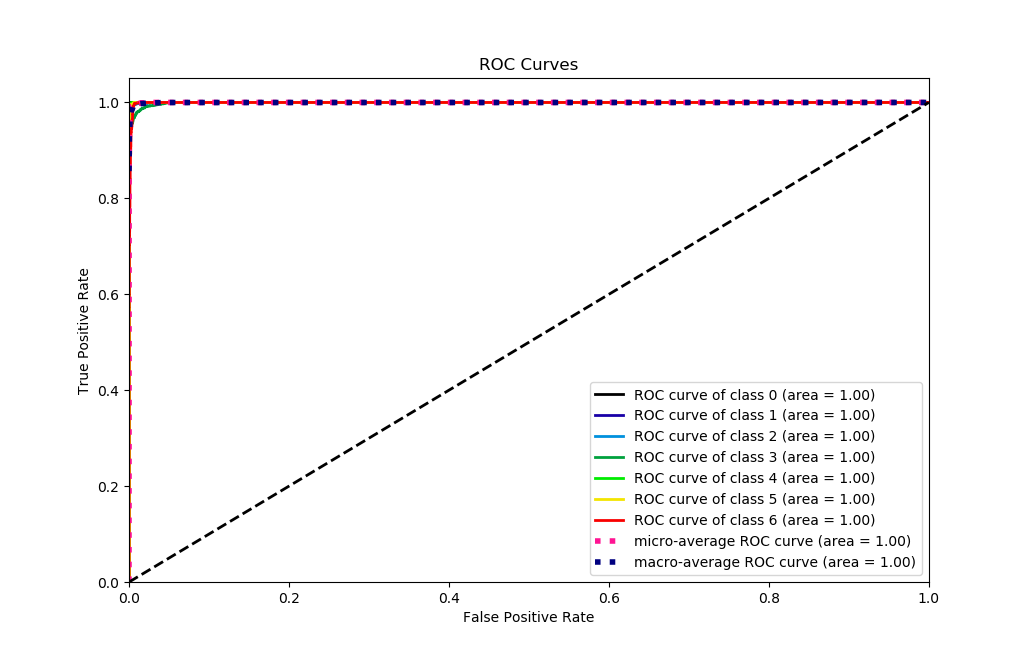
\includegraphics[height=320pt,width=330pt]{img/chapter4/rocEN.png}
                %     \caption{}
                %     \label{}
                % \end{figure}
            \item{\textbf{Arabe :} }\\
                Tout comme l'Anglais le modèle développé pour l'Arabe, a montré une capacité de prédiction très élevée. Comme on peut le voire dans le \autoref{confusion-arabe}, la confusion entre les catégories est très faible à part quelques articles des catégories proches en terme de contenu. 
                \begin{table}[H]
                    \begin{center}
                        \begin{tabular}{|c|c|c|c|c|c|c|}
                            % \cline{2-7}
                            % \hline
                            % \multicolumn{1}{c|}{} & \multicolumn{6}{|c|}{Predicted} \\
                            % \hline
                            \cline{2-7}
                            \multicolumn{1}{c|}{} & \textbf{\begin{arab}العالم\end{arab}} &  \textbf{\begin{arab}الرياضة\end{arab}} &  \textbf{\begin{arab}الجزائر\end{arab}} &  \textbf{\begin{arab}المجتمع\end{arab}} &  \textbf{\begin{arab}الدين\end{arab}} &  \textbf{\begin{arab}الثقافة\end{arab}} \\
                            \hline
                            \textbf{\begin{arab}العالم\end{arab}} & 1232  &  1  & 11 &  51  & 18  &  3 \\
                            \textbf{\begin{arab}الرياضة\end{arab}}  & 1 & 1609  &  1  &  6  &  3 &   0 \\
                            \textbf{\begin{arab}الجزائر\end{arab}}  & 28  &  2 & 587 &  21  &  9  & 17 \\
                            \textbf{\begin{arab}المجتمع\end{arab}}  & 43  & 11 &  17& 1447 &  12 &  11 \\
                            \textbf{\begin{arab}الدين\end{arab}}  & 36  &  0  &  6 &  18 & 788 &  12 \\
                            \textbf{\begin{arab}الثقافة\end{arab}}  & 3  &  0 &   8 & 53  &  9 & 436 \\
                            \hline
                        \end{tabular}
                    \end{center}
                    \caption{Matrice de confusion du modèle de la catégorisation d'articles Arabe}
                    \label{confusion-arabe}
                \end{table}

                % \item{Courbe ROC : }
                % \begin{figure}[H]
                %     \centering
                %     \includegraphics[height=320pt,width=330pt]{img/chapter4/ux/1.png}
                %     \caption{}
                %     \label{}
                % \end{figure}
        \end{itemize}

\section{Résumé automatique}
    La deuxième partie de la phase de réalisation est consacrée au résumé automatique. Nous avons expérimentés plusieurs techniques et méthodes que nous allons voire en détails dans cette section. 
    \subsection{Approches expérimentées}
        \subsubsection{Résumé extractif par Apprentissage Supervisé}
            Nous avons commencé par une approche basée sur l'apprentissage automatique supervisé, ce qui nécessitait des corpus d'articles avec leur résumés types.
            \begin{itemize}
                 \item{\textbf{Contribution à la récolte de données : "Sumrized" et "Mou3in"}}\\
                Face au manque flagrant des corpus (gratuits) pour le résumé automatique, nous avons développer une plate-forme contributive sur le web baptisée \textbf{Sumrized.com} pour la récolte des textes et des résumés en trois langues Arabe, Anglais et Français. 

                Chaque texte et son résumé sont vérifier manuellement par un expert qui peut consulter et valider les contributions à partir d'un Dashboard dédié à cet effet. L'interface principale de la plate-forme, qui est en ligne depuis Février 2018, est présentée dans la figure \ref{sumrized-ui}. 

                \begin{figure}[H]
                    \centering
                    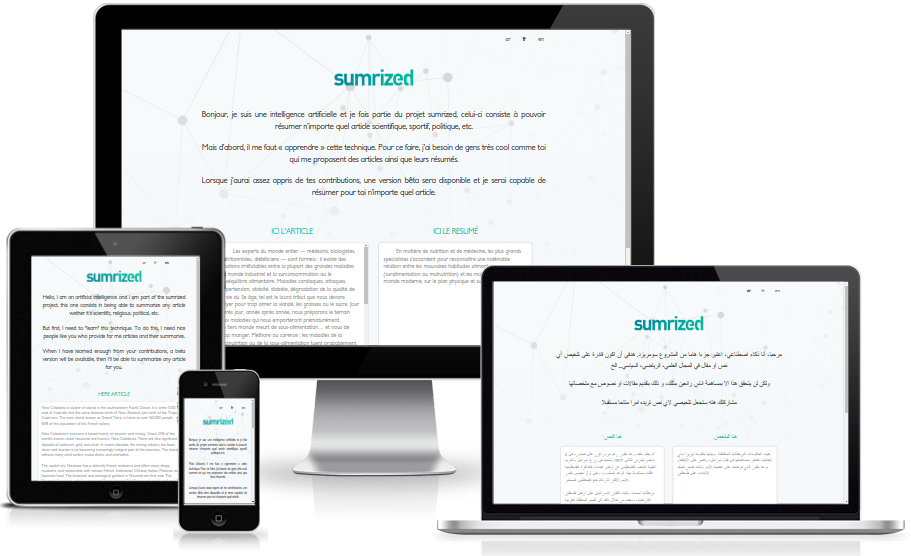
\includegraphics[height=180pt,width=320pt]{img/chapter4/sumrized/responsive.png}
                    \caption{La plate-forme Sumrized sur les différents supports}
                    \label{sumrized-ui}
                \end{figure} 

                Nous avons également développé une application de bureau, appelée \textbf{Mou3in}, afin de faciliter l'annotation des textes, elle offre à son utilisateur la possibilité d'attribuer une étiquette à chaque phrase selon son jugement (à supprimer ou à laisser). La figure \ref{mou3in} présente l'espace de travail sur l'application "Mou3in" :
                \begin{figure}[H]
                    \centering
                    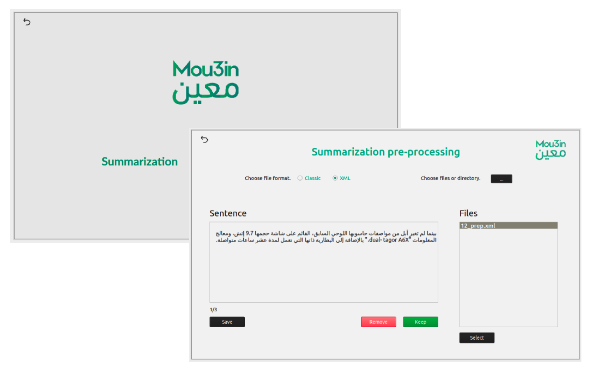
\includegraphics[height=230pt,width=370pt]{img/chapter4/mou3in/mou3in.png}
                    \caption{Interface utilisateur de "Mou3in"}
                    \label{mou3in}
                \end{figure}

                \item{\textbf{Pré-traitement et structure du dataset}}\\
                Tout les articles du dataset sont sous le format XML, chaque article a son propre identifiant et divisé en paquets de phrases selon l'opération effectuée. Ci-après la figure \ref{xml-structure} qui montre un exemple du dataset : 
                \begin{figure}[H]
                    \centering
                    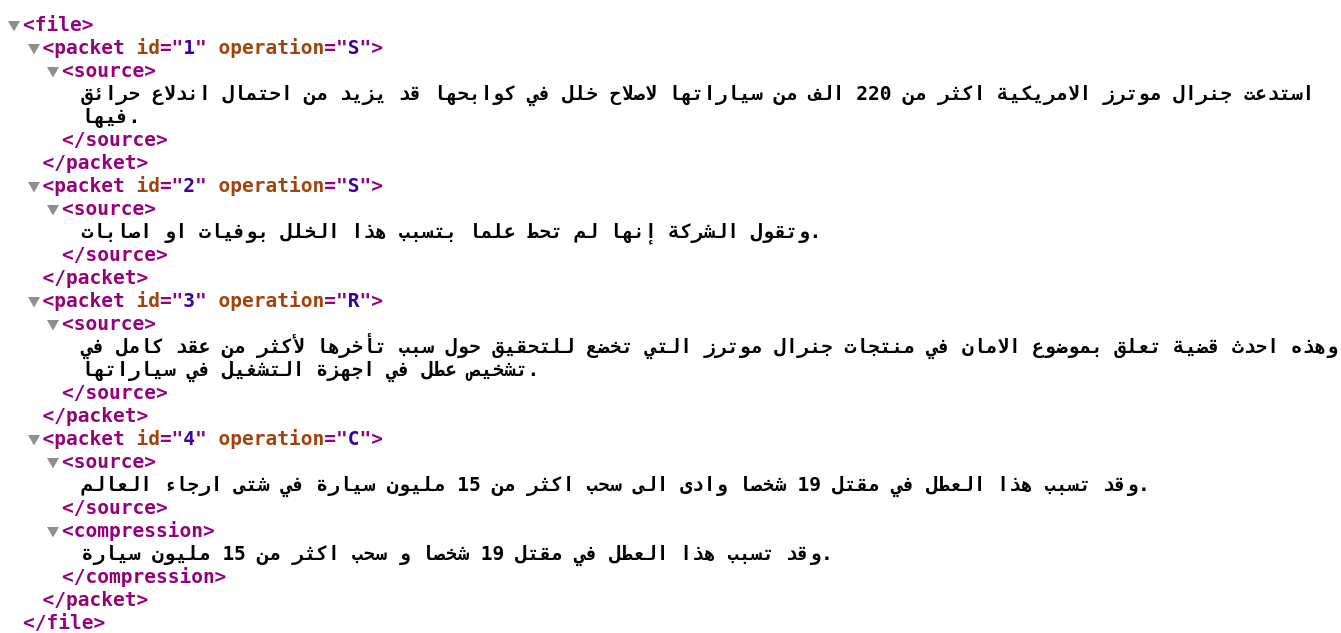
\includegraphics[height=220pt,width=430pt]{img/chapter4/xml.png}
                    \caption{Structure d'un article du dataset}
                    \label{xml-structure}
                \end{figure}
                L'approche basée sur l'apprentissage automatique demandait un très grand nombre d'articles résumés, ce qui nous a poussé à l'abandonner.
            \end{itemize}
        \subsubsection{Résumé extractif par Machine de Boltzman}
            L'approche proposée dans \cite{boltzman} utilise un modèle d'apprentissage profond afin de prédire les phrases les plus importantes dans un texte donnée en utilisant 9 caractéristiques sur chaque phrase. Elle consiste en trois grande phases: l'extraction des caractéristiques, la conversion en valeurs numériques et la génération du résumé à partir des scores de chaque phrase. 

            \begin{itemize}[leftmargin=*]
                \item{\textbf{Pré-traitement et structure du dataset}}\\
                Cette méthode, contrairement aux autres, est appliquée sur un seul document, on a pas besoin de plusieurs documents. La texte est segmenté en phrase, chaque phrase est divisé en mots et les caractéristiques citées là-dessus sont calculées.\\

                La matrice qui représentent le texte est injectée dans une Machine de Boltzman\footnote{Type de réseau de neurones artificiels pour l'apprentissage non supervisé} afin de calculé les score des phrases. Les résultats sont triés dans l'ordre décroissant des scores et le résumé est établi selon ces derniers.\\

                \item{\textbf{Résultats et critiques}}\\
                L'évaluation de ce modèle est effectuée en utilisant le \emph{Gold Standard}\footnote{Dataset de référence construit par des experts linguistes, utilisé pour l'évaluation des résultats} Duc2004 qui est un dataset qui contient 50 articles de presse de différentes catégories et 4 à 5 résumés de référence pour chaque article.

                Nous avons obtenu les résultats présentés dans le \autoref{result-boltzman} en utilisant ROUGE (les métriques d'évaluations, ROUGE notamment, sont définies dans la \autoref{metrique-eval}) : 
                \begin{table}[H]
                    \begin{center}
                        \begin{tabular}{|c|C{1.2cm}|C{1.2cm}|C{1.2cm}|C{1.2cm}|C{1.2cm}|C{1.2cm}|C{1.2cm}|C{1.2cm}|}
                            \cline{2-9}
                            \multicolumn{1}{c|}{} & \textbf{R-1} &  \textbf{R-2} &  \textbf{R-3} &  \textbf{R-4} &  \textbf{R-L} &  \textbf{R-W} &  \textbf{R-S} &  \textbf{R-SU} \\
                            \hline
                            \textbf{Rappel} & 0.4172 & 0.0615 & 0.0129 & 0.0042 & 0.3239 & 0.1089 & 0.1693 & 0.1739 \\
                            \textbf{Précision} & 0.1982 & 0.0264 & 0.0054 & 0.0016 & 0.1525 & 0.0919 & 0.0385 & 0.0402 \\
                            \textbf{F-mesure} & 0.2549 & 0.0346 & 0.0071 & 0.0022 & 0.1963 & 0.0934 & 0.0556 & 0.0578 \\
                            \hline
                        \end{tabular}
                    \end{center}
                    \caption{Résultats du résumeur extractif basé sur la Machine de Boltzman}
                    \label{result-boltzman}
                \end{table}
                En effet, ces résultats sont très proches des résumeurs de l'état de l'art, mais le modèle que nous avons utilisé est pré-entraîné sur un type de données totalement différent (des images), ce qui nous a amené à laisser tomber cette approche.   
            \end{itemize}

        \subsubsection{Résumé extractif par Plongement de mots\ref{plongement}}
        L'approche proposée par l'équipe de recherche du département informatique de l'Université de Bari en Italie \cite{bari}, est basée sur la similarité textuelle entre la phrase centroïde et les autres phrases du texte en utilisant les plongements de mots (Word embeddings). La conception et l'algorithme de réalisation sont détaillés dans \ref{plongement}       

    \subsection{Résultats et évaluation}
        \subsubsection{Métrique d'évaluation : ROUGE\label{metrique-eval}}
        ROUGE est l'acronyme de "Recall-Oriented Understudy for Gisting Evaluation". Il s'agit essentiellement d'un ensemble de métriques permettant d'évaluer le résumé automatique de textes ainsi que la traduction automatique. Il fonctionne en comparant un résumé produit automatiquement ou une traduction à un ensemble de résumés de référence (généralement produits par des humains). \cite{rouge0}
    
        \subsubsection{Types des métriques de ROUGE\label{type-rouge}}
        \begin{itemize}
            \item{ROUGE-1, 2, 3 et 4 : font référence au chevauchement des uni-grammes, bi-grammes, tri-grammes et quadri-grammes, respectivement, entre le système et les résumés de référence \cite{rouge1}.}\\
            \item{ROUGE-L, W : basés sur la plus longue sous-séquence commune (LCS) \cite{rouge2}.}\\
            \item{ROUGE-S : basé sur les cooccurrences des paires de mots dans l'ordre des phrases \cite{rouge2}.}\\
            \item{ROUGE-SU : en plus des paires de mots, il utilise aussi la cooccurrence mot unique toujours dans l'ordre des phrases.}
        \end{itemize}
    
        \subsubsection{Résultats du modèle de résumé automatique final}
        \begin{table}[H]
            \begin{center}
                \begin{tabular}{|c|C{1.2cm}|C{1.2cm}|C{1.2cm}|C{1.2cm}|C{1.2cm}|C{1.2cm}|C{1.2cm}|C{1.2cm}|}
                    \cline{2-9}
                    \multicolumn{1}{c|}{} & \textbf{R-1} &  \textbf{R-2} &  \textbf{R-3} &  \textbf{R-4} &  \textbf{R-L} &  \textbf{R-W} &  \textbf{R-S} &  \textbf{R-SU} \\
                    \hline
                    \textbf{Rappel} & 0.5631 & 0.1226 & 0.0346 & 0.0139 & 0.5111 & 0.1729 & 0.2981 & 0.3029 \\
                    \textbf{Précision} & 0.1662 & 0.0361 & 0.0105 & 0.0042 & 0.1503 & 0.0912 & 0.0281 & 0.0289 \\
                    \textbf{F-mesure} & 0.2485 & 0.0541 & 0.0157 & 0.0063 & 0.2245 & 0.1145 & 0.0488 & 0.0503 \\
                    \hline
                \end{tabular}
             \end{center}
            \caption{Résultats du résumeur extractif basé sur le plongement de mots}
            \label{result-boltzman}
        \end{table}

\section{Traduction Automatique}
Comme il a été décrit dans le chapitre précédent, la traduction sera intégrée directement à l'application finale afin d'offrir une fonctionnalité de traduction en plus de celle du résumé et la catégorisation. A cet effet, nous avons utilisé la bibliothèque TextBlob qui offre une traduction multilingues d'un article ou d'un résumé.
    \subsection{Exemple de traduction automatique}
    \begin{itemize}
        \item Anglais :\\ 
        \textquotedbl The Interior Ministers of Spain and Algeria signed an agreement this week to form a joint team of investigation with the goals of fighting “illegal migration” and “preventing Islamist terrorism.” The agreement comes after recent crackdowns by the Algerian authorities during the first months of 2018 have reduced the number of undocumented Algerian migrants arriving in Spain, a reduction that was praised by the Spanish Interior Minister Juan Ignacio Zoido at their meeting in Madrid.\textquotedbl \\
        
        \item Arabe :\\
        \textquotedbl وقع وزيرا الداخلية الإسباني والجزائري اتفاقا هذا الأسبوع لتشكيل فريق مشترك من التحقيق بهدف محاربة "الهجرة غير الشرعية" و "منع الإرهاب الإسلامي". ويأتي هذا الاتفاق بعد الإجراءات القمعية الأخيرة التي قامت بها السلطات الجزائرية خلال الأشهر الأولى من خفّض عام 2018 عدد المهاجرين الجزائريين غير الشرعيين الذين وصلوا إلى إسبانيا ، وهو تخفيض أشاد به وزير الداخلية الإسباني خوان إغناسيو زويدو في اجتماعهم في مدريد. \textquotedbl
    
        \item Français :\\
        \textquotedbl Les ministres de l'Intérieur d'Espagne et d'Algérie ont signé cette semaine un accord pour former une équipe conjointe d'enquête ayant pour objectif de lutter contre les "migrations clandestines" et "la prévention du terrorisme islamiste." L'accord intervient après les récentes mesures de répression des autorités algériennes. 2018 ont réduit le nombre de migrants algériens sans papiers arrivant en Espagne, une réduction qui a été saluée par le ministre espagnol de l'Intérieur Juan Ignacio Zoido lors de leur réunion à Madrid.\textquotedbl \\

   \end{itemize}

\chapter*{Conclusion et perspectives}    
%!TEX program=luatex

Aujourd’hui, les internautes se retrouvent quotidiennement face à un flux d’informations massif et une diversité de contenu très importante, et les médias et sites d’actualité y contribuent pleinement. Dans un environnement où l'utilisateur ne dispose toujours pas de moyen satisfaisant pour gérer ce flux, un nouveau besoin se crée, celui d’une expérience de lecture personnalisée, correspondant le plus pertinemment et efficacement aux besoins et centres d’intérêt de l’utilisateur.
 
La première motivation de ce travail été de fournir un outil qui permet au lecteur de faire sa revue de presse quotidienne de la façon la plus efficace et la plus enrichissante possible.
 
Nous réalisons à présent qu’entreprendre ce projet s'étend bien au-delà du cadre d’un projet de fin d'études et s'inscrit dans une optique d'innovation, dont l’objectif est d'apporter une réelle contribution et valeur ajoutée à toutes les solutions existantes.
 
Dans le présent mémoire, nous avons examiné en premier lieu la littérature des systèmes de recommandation tout en explicitant les différents concepts liés au profilage utilisateur. Et ce, afin d'enlever l’ambiguïté quant à ses différents usages pour bien cerner les possibilités d'exploitation de ses techniques.
 
Nous avons ensuite effectué un long travail de recherche sur l'état de l'art du traitement automatique du langage naturel. Nous avons ainsi identifié les travaux les plus fiables, les différentes techniques utilisées et les outils les plus performants.
 
Une longue période du projet a été dédiée à la recherche, la récolte et le pré-traitement des données. Une fois les datasets de chaque application créés, une étude exploratoire a été effectuée sur ces derniers afin de détecter les composants homogènes des données disponibles et de mettre en évidence les indicateurs discriminants des instances des corpus.

Néanmoins, un des principaux freins au projet a été le manque flagrant de références, de corpus et d'outils pour le traitement automatique de la langue arabe. Un travail conséquent a été effectué pour le pré-traitement et la préparation des datasets, liés à l’aberration et la particularité de cette langue.
 
Nous avons également présenté la conception de la solution proposée, détaillé les différentes démarches suivies et défini les approches adoptées, tout en justifiant les choix entrepris, leurs avantages et leurs inconvénients.
 
La dernière phase aborde l'implémentation et l'intégration des différents modules, dans laquelle nous avons présenté une étude comparative des modèles d'apprentissage automatique développés pour chacune des quatre problématiques principales : la catégorisation, le résumé automatique, la traduction automatique et la recommandation d'articles de presse. Nous avons par la suite présenté les résultats obtenus et évalué ces derniers en utilisant les mesures et les métriques adéquates.
 
Les résultats de la classification d'articles de presse ont été très satisfaisants comparés aux travaux similaires. Les modèles inférés pour la prédiction des catégories ont donné un taux de précision de 99\%. Nous avons également eu de très bons résultats quant au résumé automatique dans les deux langues.
 
La dernière étape de notre projet a été la réalisation de l'application \textquotedbl Feedny\textquotedbl.\\
\textquotedbl Feedny\textquotedbl est une application mobile qui intègre tous les modèles développés, elle permet au lecteur d'exploiter toutes les fonctionnalités présentées précédemment. L'expérience utilisateur et le design des interfaces ont été conçus de telle sorte à compléter les fonctionnalités par l'intuitivité et le plaisir de l'utilisation.
 
La dernière partie du mémoire présente les fonctionnalités et interfaces de l'application ainsi que les différentes phases du développement en justifiant le choix des outils et les langages de programmation.
 
Nous pouvons aujourd’hui dire que notre objectif a été atteint, puisque l’application que nous avons réalisée satisfait largement les principales ambitions définies.
 
Ce projet nous a été bénéfique sur plusieurs plans. Il nous a permis de mettre en pratique toutes les connaissances acquises lors de notre cursus de master en Systèmes Informatiques Intelligents, de développer une méthodologie de recherche et de distinction des travaux, d'élargir les notions théoriques dans le TALN, l'apprentissage automatique et la recherche d'informations, et de nous initier aux systèmes de recommandations d'articles de presse. Le mémoire nous a permis d'améliorer notre capacité rédactionnelle et de devenir plus rigoureux quant aux questions de plagiat, des sources d'informations et de leur référencement. Le travail en binôme, supervisé par notre promotteur à renforcer notre capacité à travailler en équipe.
 
Toutefois, il est très important de signaler que la solution proposée reste largement perfectible. Plusieurs points demandent encore à être revus et retravaillés. L'une des perspectives qui pourraient s'avérer intéressantes serait de construire un large corpus pour le résumé automatique abstractif, afin de donner plus d'exactitude aux résumés générés. Il serait très utile aussi d'ajouter d'autres catégories d'articles de presse, cela donnera plus de diversité au contenu proposé. Les modèles de classification d'articles pourraient être améliorés afin de s'adapter aux vocabulaires récents et de prendre en charge les nouveaux mots du langage (Brexit, Facebooker, etc.).

% Notre système de recommandation doit être évalué dans le future, dés que le nombre d'utilisateurs et interactions le permettenet
Quant à l'application \textquotedbl Feedny\textquotedbl, elle pourrait être enrichie également par d'autres fonctionnalités telles que l'ajout de nouvelles sources d'articles de presse par l'utilisateur. Mais aussi par le fait de proposer plusieurs sources pour un même sujet d'article afin d'identifier les sources les plus fiables et objectives.
Et bien sûr, l’application ne gagnerait que plus d’utilisateurs et ne deviendrait que plus accessible si une plateforme web de la solution est développée.
\newpage
\pagenumbering{roman} 
\bibliographystyle{unsrt} 
\bibliography{ref}

\end{document}
%~~~END~~~%